%%%%%%%%%%%%%%%%%%%%%%%%%%%%%%%%%%%%%%%%%%%%%%%%%%%%%%%%%%%%%%%%%%%%%%%%%%
%% This is a document template for an Otago thesis (Masters or PhD).

%%
%% Look in the directory example_document for filled-out Chapters
%% that show you how to do figures, bibliographies, and tables.
%%
%% Since this was written for Computer Science at Otago University,
%% Harvard (author, date) style citations are used.  Other students
%% should consult their advisors as to what style of citations to use.  
%%
%% Nathan Rountree 9/2/98
%%
%%%%%%%%%%%%%%%%%%%%%%%%%%%%%%%%%%%%%%%%%%%%%%%%%%%%%%%%%%%%%%%%%%%%%%%%%%%

%%
%% In the style of a technical report, in 12pt and one sided.
%% Start Chapters on right hand side pages only.
%%
\documentclass[12pt]{report}    
%%\documentclass[12pt,twoside,openright]{report} %% Use this for twosided.

%%
%% Load packages.
%%
\usepackage[phd]{otagothesis}     %% Use Otago page layout

%\usepackage[natbib, mincitenames=3, maxcitenames=11, style=apa]{biblatex}
%\usepackage[longnamesfirst,round]{natbib} %% Use Natural Sciences bibliography
\usepackage[round, sort]{natbib} %% Use Natural Sciences bibliography
%enable abbreviated in text citations
\usepackage{etoolbox}

\newif\ifabbreviation
\pretocmd{\thebibliography}{\abbreviationfalse}{}{}
\AtBeginDocument{\abbreviationtrue}
\DeclareRobustCommand\acroauthor[2]{%
  \ifabbreviation #2\else #1 (\mbox{#2})\fi}

%%\usepackage{times}              %% Times PostScript font. Don't use
				  %% if thesis contains lots of math.

\usepackage{graphicx}             %% jpg, gif, tiff, and pdf graphics
\usepackage{moreverb}             %% Verbatim Code Listings
\usepackage{hyperref}             %% hyperlinks
%\usepackage{color}
\usepackage{xcolor}
\usepackage{supertabular}
\usepackage{tabularx}
\usepackage{array}
\usepackage{multicol}
\usepackage{colortbl}
\usepackage{textcomp}
\usepackage{nomencl}

\usepackage{tikz} %arrows
\usepackage{mathtools}
\usepackage{pstricks}

%\usepackage{subfigure}
\usepackage{subcaption}
\usepackage{mdframed} %frame with caption
%Sepackage[export]{adjustbox} %frame figures
\usepackage{cleveref}
%\usepackage{mwe}
\usepackage{multirow}
%\usepackage{booktabs}
\usepackage{longtable}


\usepackage{titlesec}
\usepackage{titlesec}

%\usepackage{etoolbox}
%\makeatletter
%\patchcmd{\ttlh@hang}{\parindent\z@}{\parindent\z@\leavevmode}{}{}
%\patchcmd{\ttlh@hang}{\noindent}{}{}{}
%\makeatother

%%spaceing for Chapter headers
\titleformat{\Chapter}[display]   
{\normalfont\huge\bfseries}{\Chaptertitlename\ \theChapter}{10pt}{\Huge}   
\titlespacing*{\Chapter}{0pt}{0pt}{20pt}

%add subsubsubsection
\titleclass{\subsubsubsection}{straight}[\subsection]

\newcounter{subsubsubsection}[subsubsection]
\renewcommand\thesubsubsubsection{\thesubsubsection.\arabic{subsubsubsection}}
\renewcommand\theparagraph{\thesubsubsubsection.\arabic{paragraph}} % optional; useful if paragraphs are to be numbered

\titleformat{\subsubsubsection}
  {\normalfont\normalsize\bfseries}{\thesubsubsubsection}{1em}{}
  \titlespacing*{\subsubsubsection}
  {0pt}{3.25ex plus 1ex minus .2ex}{1.5ex plus .2ex}

\makeatletter
\renewcommand\paragraph{\@startsection{paragraph}{5}{\z@}%
  {3.25ex \@plus1ex \@minus.2ex}%
  {-1em}%
  {\normalfont\normalsize\bfseries}}
\renewcommand\subparagraph{\@startsection{subparagraph}{6}{\parindent}%
  {3.25ex \@plus1ex \@minus .2ex}%
  {-1em}%
  {\normalfont\normalsize\bfseries}}
\def\toclevel@subsubsubsection{4}
\def\toclevel@paragraph{5}
\def\toclevel@paragraph{6}
\def\l@subsubsubsection{\@dottedtocline{4}{9em}{5em}}
\def\l@paragraph{\@dottedtocline{5}{10em}{12em}}
\def\l@subparagraph{\@dottedtocline{6}{15em}{6em}}
\makeatother

%enable subsubsubsection to TOC
\setcounter{secnumdepth}{4}
\setcounter{tocdepth}{4}
%\usepackage{float}


%remove figures
%\def\includegraphic{}
%\def\includegraphics{}
%\def\input{}

\usepackage{lipsum} 


%%
%% Set title, author and date.
%%
\title{A Bioinformatics Approach to Synthetic Lethal Interactions in Breast Cancer with Gene Expression Data}
\author{S. Thomas Kelly}
\date{31 March 2017}

%%
%% The library want to know all sorts of personal stuff!
%% Can be left out if you don't use the \frontstuff command
%%
\fullname{Simon Thomas Kelly}
\department{Department of Biochemistry}
\dob{24 February 1992} %% date-of-birth
\address{710 Cumberland Street, Dunedin, NZ}

%%
%% Uncomment to just print up a few Chapters.
%%
%%\includeonly{literature,conclusion}

%%
%% Go!
%%
\begin{document}

%%
%% Put in titlepage and contents, etc...
%%
\setcounter{tocdepth}{4} %%display subsubsubheadings

%\frontstuff

\tableofcontents
\listoffigures
\listoftables

%%
%% Set to one-and-a-half line-spacing
%%
\linespread{1.3} \normalsize

%%

%% These lines assume there are files called intro.tex, literature.tex etc.
%%

%%methods
\setcounter{Chapter}{1}
\chapter{Methods and Resources}
\label{chap:methods}

%\section{Overview/meta-text}
In this chapter, I will outline the various existing resources and methods utilised throughout this project. This includes public data repositories, stable and development releases of software packages (mostly for the R programming environment), and implementation of bioinformatics methods and statistical concepts with Shell or R scripts developed for this purpose. Methods and packages developed specifically for this project will be covered in more detail along with preliminary data to demonstrate and support their use in chapter 3. 

\section{Bioinformatics Resources for Genomics Research}
\subsection{Public Data and Software Packages}
Various bioinformatics resources, such as databases and methods, have become integral parts of genetics and genomics research. Reference genomes, genotyped variants, gene expression, and epigenetics profiles are among the most commonly used resources. Gene expression data in particular is widely available from many microarray and RNA-Seq studies, from repositories such as Gene Expression Omnibus (GEO) \citep{GEO2016}, caArray \citep{caArray2014}, and ArrayExpress \citep{ArrayExpress2013}. Such profiles are excellent resources to examine the changes of gene expression occurring in cancers and the variation between samples. These microarray initiatives have set a precedent for data sharing, data mining, and the wider benefits of publicly available data for enabling the scientific community to further utilise the data rather than a single research group or consortium \citep{Rung2013}. The practice of integrating findings from publicly available genomics data with the research questions and experimental results of individual research groups has carried over into RNA-Seq datasets including the large-scale cancer genomics projects \citep{ICGC2011}. This thesis is one such example of an investigation enabled by this wider movement and tools developed in various disciplines to generate, process, and disseminate genomic-scale data.
 
Along with databases, it is also becoming common practice for bioinformatics researchers to release their code as open-source or provide a software package to enable replication of the findings or further applications of the methods \citep{Stajich2006}. This is part of a wider movement in software and data analysis with many tools to facilitate such work being released for use in Linux or the R programming environment \citep{R_core}. In addition to the R packages hosted on CRAN \citep{CRAN}, the Bioconductor repositories \citep{Gentleman2004} also contain many packages specifically for applications in bioinformatics, and the GitHub site hosts many packages in various stages of development and early release. Packages from these various sources have been used throughout this project and cited where-ever possible. Several R packages have been developed during this thesis project and either publicly released on GitHub or prepared to accompany a publication.

\subsubsection{Cancer Genome Atlas Data}
Molecular profile data from normal and tumour samples was downloaded from publicly available sources, using the TCGA \citep{TCGA2012} and the International Cancer Genome Consortium (ICGC) web portals \citep{ICGC2011}. These include gene expression (RNA-Seq), somatic mutations, and anonymous clinical data. These versions downloaded were on Aug 6th 2015 (Release 19) and May 2nd 2016 (Release 20) for breast and stomach cancer respectively via the ICGC data portal (\url{https://dcc.icgc.org/}).
%%The Cancer Genome Altas project supports a wide range of cancers including gene expression for breast invasive adenocarcinoma with 600 samples (63 normal, 534 primary tumour, and 3 metastases) available the AligentG4502 244K cDNA microarray mapping 17811 genes \citep{TCGA2012}. TCGA provides microarray expression data processed with loess normalisation and integrated to give an expression call for each gene. %% Array data removed

Performing a genomic alignment in remains a challenge in bioinformatics and methods to do so may yet be improved \citep{Chen2010}. However, the statistical and biological aspects of bioinformatics are the focus of this thesis, comparing alignment methods is outside the scope of these investigations. The TCGA project \citep{TCGA2012} used widely adopted tools: ``Bowtie''  for alignment \citep{bowtie}, ``mapslice'' to detect splice sites \citep{mapsplice}, and the Reads Per Kilobase per Million mapped reads (RPKM) approach to qualify reads per transcript as a measure of gene expression \citep{Mortazavi2008}. These are widely acceptable tools for processing RNA-Seq data which were used to produce the raw counts of mapped reads (tier 1) and normalised expression data (tier 3) publicly available from TCGA.

Raw count and RSEM normalised TCGA expression data from Illumina RNA-Seq protocols were available from 1,177 samples (113 normal, 1,057 primary tumour, and 7 metastases) for 20,501 genes. TCGA somatic mutation data for 981 samples (976 primary tumours and 5 metastases) across 25,836 genes were available including 969 samples (964 primary tumours and 5 metastases) with corresponding RNA-Seq expression data and 19,166 genes mapped from Ensembl identifiers to gene symbols, of which 16,156 had corresponding gene expression information. Unless otherwise stated, the raw counts were used for further processing rather than the RSEM normalised data (provided by TCGA tier 3).

\subsubsection{Reactome and Annotation Data} \label{methods:gene_set}

Unless otherwise specified, pathway analysis was performed for human pathway annotation from the Reactome database (version 52) with pathway gene sets derived from the \texttt{reactome.db} R package. Entrez identifiers were mapped to gene symbols or aliases to match to TCGA expression and mutation data using the \texttt{org.Hs.eg.db} R package. Further pathway analysis used breast cancer gene signatures from Gatza and colleagues (Gatza \textit{et al}., 2011; Gatza \textit{et al}., 2014). These gene symbols were matched to the relevant dataset and used to construct a matrix of category membership using the \texttt{safe} R package \citep{safe}.

\section{Data Handling}

\subsection{Normalisation}

Apart from the PAM50 subtyping procedure \citep{Parker2009}, which required RSEM normalised data (J.S. Parker personal communication), the analysis of the RNA-Seq data presented here was based on raw read count data. Raw read counts were log-scaled; samples removed for consistency (based on a Euclidean distance correlation matrix as described in section \ref{methods:sample_qc}); and the final dataset was TMM normalised \citep{Robinson2010} then processed using the \texttt{voom} function \citep{Law2014} in the \texttt{limma} R package \citep{limma}.

\begin{figure}[!ht]
\begin{mdframed}
   %\resizebox{1 \textwidth}{!}{
   \begin{center}
%
       \subfigure[Raw counts (log-scale)]{%
            \label{fig:density:first}
            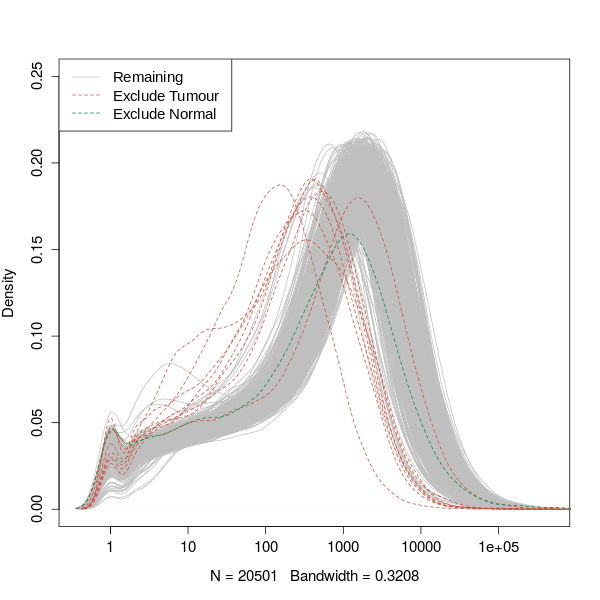
\includegraphics[width=0.4\textwidth]{fig2a.png}
        }%
        \subfigure[Voom normalised]{%
           \label{fig:density:second}
           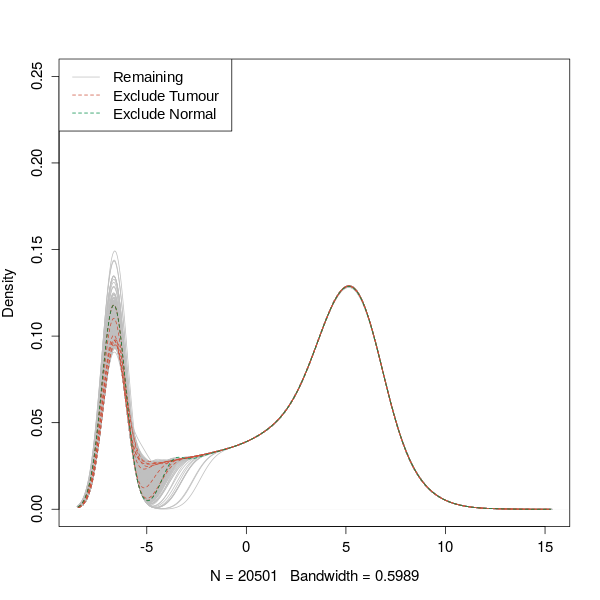
\includegraphics[width=0.4\textwidth]{fig2b.png}
        }%
%
\end{center}
\caption[Read count density]{\small \textbf{Read count density.} Sample density plots of raw counts on log-scale and voom normalised showing samples removed due to quality concerns.}
%}
\label{fig:density}
\end{mdframed}
\end{figure}

\begin{figure*}[!ht]
\begin{mdframed}
%  \resizebox{\textwidth}{!}{
         \begin{center}
%
        \subfigure[Mean raw counts (log-scale)]{%
            \label{fig:mean:first}
            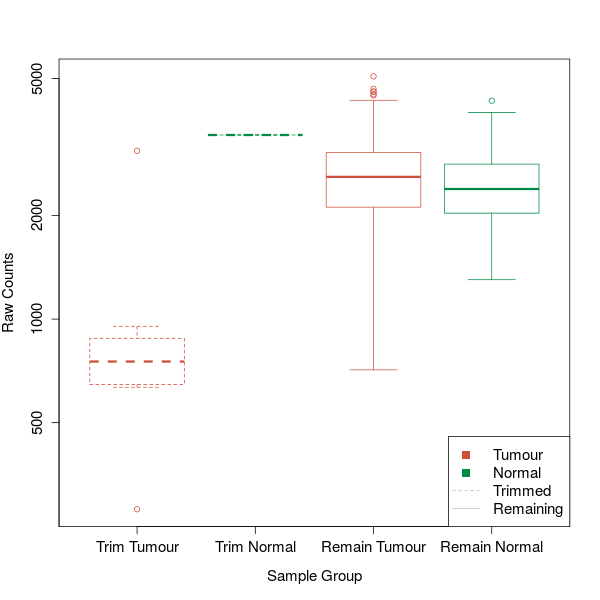
\includegraphics[width=0.4\textwidth]{fig3a.png}
        }%
        \subfigure[Mean voom normalised]{%
           \label{fig:mean:second}
           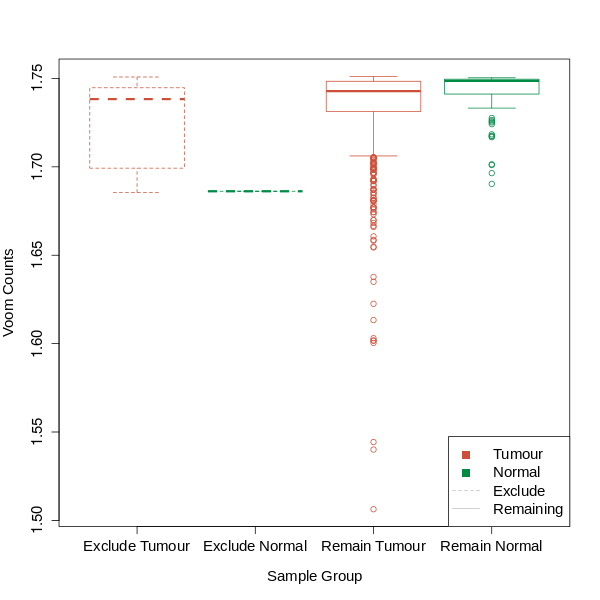
\includegraphics[width=0.4\textwidth]{fig3b.png}
        }%
%
    \end{center}
  \caption[Read count sample mean]{\small \textbf{Read count sample mean.} Boxplots of sample means for raw counts on log-scale and voom normalised show removed tumour samples with low mean read count.}
%}
\label{fig:boxplot}
\end{mdframed}
\end{figure*}


\subsection{Sample Triage} \label{methods:sample_qc}

The TCGA RNA-Seq data were assessed for batch effects using a correlation matrix of the log-transformed raw counts for which a heatmap (Euclidean distance, complete linkage) is shown in Figure \ref{fig:corr_map}. While no major batch effects were detectable between the samples, 9 samples were excluded due to poor correlation with the remaining samples, as detailed in Table \ref{tab:qc}. These samples showed unusual density plots compared to the rest of the dataset, and exhibited low mean read count in Figures \ref{fig:density} and \ref{fig:boxplot}. A heatmap showing key clinical properties of these excluded samples and their correlation with the remainder of the samples is shown in Figure \ref{fig:corr_map_part}, and a full correlation heatmap (Figure \ref{fig:corr_map}) shows these samples as relatively poorly correlated outliers in the bottom rows and left columns.
%In both of these cases, a shared tissue source site or patient donor indicates that variations in sample preparation are likely behind the outlying expression profiles. The Christiana Healthcare patients were sequenced in triplicate when replicate samples were rare in this dataset suggesting there were suspected errors in these samples during data generation which have lower mean read count than most of the dataset. %tangent
%Clinical characteristics over-represented in removed samples were ER+, ductal, state 2, luminal A or basal type tumours but these are the most common in the dataset. %relevance
After removal of these samples, the TCGA dataset used for analysis consisted of the remaining 1168 samples (from 1040 patients): 1049 tumour samples, 112 normal tissue for matched samples, and 7 metastases.

\begin{table*}[!ht]
\caption{Excluded Samples by Batch and Clinical Characteristics.}
\label{tab:qc}
\resizebox{\textwidth}{!}{
      \begin{tabular}{sc^c^c^c^c^c^c^c^c^c^c^c^c}
      \rowstyle{\bfseries}
        \multicolumn{1}{c}{\bfseries Tissue Source}		& \multicolumn{1}{sc}{\bfseries Type}   & \multicolumn{1}{sc}{\bfseries Batch} & \multicolumn{1}{sc}{\bfseries Plate} & \multicolumn{1}{sc}{\bfseries Patient} & \multicolumn{1}{sc}{\bfseries Samples} & \multicolumn{1}{c}{\bfseries p53}      & \multicolumn{1}{sc}{\bfseries Subtype}   & \multicolumn{2}{sc}{\bfseries Treatment (History)}	& \multicolumn{3}{sc}{\bfseries Clinical Subtypes (Stage)} \\
        \hline
       \rowcolor{black!10}
        A7 Christiana		& Tumour & 47	 & A227  & A0DB  &  1 of 3   & NA       & Luminal A & Mastectomy & (no)				& ER$+$  &  Ductal   	& (2)        \\
       \rowcolor{black!5}
        A7 Christiana		& Tumour & 96	 & A220  & A13D  &  1 of 3   & Wildtype & Luminal A & Mastectomy & (no)				& ER$+$  &  Ductal   	& (2)        \\
       \rowcolor{black!10}
        A7 Christiana		& Tumour & 96	 & A227  & A13E  &  1 of 3   & NA       & Basal     & Lumpectomy & (no) 				& ER$-$  &  Ductal   	& (2)        \\
       \rowcolor{black!5}
        A7 Christiana		& Tumour & 142	 & A277  & A26E  &  1 of 3   & NA       & Basal     & Lumpectomy & (no) 				& ER$+$  &  Ductal   	& (2)        \\
       \rowcolor{black!10}
        A7 Christiana		& Tumour & 47	 & A277  & A0DC  &  1 of 2   & NA       & Luminal A & Mastectomy & (yes)				& ER$+$  &  Lobular   	& (3)        \\
       \rowcolor{black!5}
        A7 Christiana		& Tumour & 142	 & A220  & A26I  &  1 of 2   & Mutant   & Basal     & Lumpectomy & (yes) 				& ER$-$  &  Ductal   	& (2)        \\
       \rowcolor{black!10}
        AC Intl Genomics	& Tumour & 177	 & A18M  & A2QH  &  2 of 2   & Mutant   & Basal     & Radical Mastectomy & (no) 			& ER$-$  &  Metaplastic   & (2)        \\
       \rowcolor{black!5}
        AC Intl Genomics	& Tumour & 177	 & A220  & A2QH  &  2 of 2   & Mutant   & Basal     & Radical Mastectomy & (no) 			& ER$-$  &  Metaplastic   & (2)        \\
       \rowcolor{black!10}
        GI ABS IUPUI		& Normal & 177	 & A16F  & A2C8  &  1 of 1   & NA       & Luminal A & Radical Mastectomy and Neoadjuvant & (no) 	& ER$+$  &  Ductal   	& (2)        \\
\hline
      \end{tabular}
}
\end{table*}


\subsection{Metagenes and the Singular Value Decomposition} \label{methods:metagene}
A ``metagene'' offers a consistent signal of pathway (expression) activation or inactivation by dimension reduction of a matrix, avoiding negatively correlated genes averaging out the signal of a mean-based centroid \citep{Huang2003}. Constructing these pathway metagenes used gene sets for Reactome and Gatza signatures (Gatza \textit{et al}., 2011; Gatza \textit{et al}., 2014) as specified above (see Section \ref{methods:gene_set}). The singular-value decomposition was performed ($X = U^{T} D V$ where $X$ is the data matrix of the gene set with genes $\times$ samples) and the leading eigenvector (first column of $V$) corresponding to the largest singular value was used as a metagene for the pathway gene set. To ensure consistent directionality of metagene signals, the median of the gene set in each sample was calculated and correlated against the metagene with the (arbitrary) metagene sign adjusted as needed to conform with the majority of the gene set (i.e., positive correlation between metagene and the median-based centroid). To ensure that genes and pathways were weighted equally, metagenes were derived from a z-transformed dataset of gene expression and samples were scaled (by fractional ranking) for each metagene so that they were comparable on a $[0,1]$ scale. 

\subsubsection{Candidate Triage and Integration with Screen Data} \label{methods:venn_analysis}
Candidate triage in combination with the experimental data was intended to integrate findings of the SLIPT analysis with an ongoing experiment project \citep{Chen2014, Telford2015}. The first procedure to compare the SLIPT gene candidates for \textit{CDH1} with an siRNA experimental screen \citep{Telford2015} was a direct comparison of the overlapping candidates, presented in a Venn diagram and tested with the $\chi^2$ test. Since these candidates modestly overlapped at the gene level (even when excluding genes not contained in both datasets), further gene set over-representation analysis was performed for pathways specific to each detection approach and the intersection of the two.

The pathway composition of the intersection was further verified by a permutation resampling analysis (as described in section \ref{methods:permutation}): the same number of genes detected by SLIPT were sampled randomly from the universe of genes tested by both approaches. These samplings were performed over 1 million iterations and the pathway over-representation was compared for each of the 1,652 reactome pathways.
%Adjusting for multiple comparisons was not needed here in a permutation analysis as the test $\chi^2$ statistics were directly used with the same degrees of freedom between expected and observed.
These over-representation scores ($\chi^2$) were compared the observed over-representation in the intersection of the SLIPT candidates, with the proportion of resamplings with higher $\chi^2$ values used for empirical p-values of pathway composition. Pathways for which no resamplings were occurred as high as the observed were reported as $p < 10^{-6}$. These empirical p-values were adjusted for multiple comparisons (FDR). Intersection size was not assumed to be constant across resamplings so similarly with the proportion of resamplings with higher or lower intersection size were used to evaluate significance of enrichment or depletion respectively (of siRNA candidate among SLIPT candidate genes).  

\section{Techniques}
Various statistical, computational, and bioinformatics techniques were performed throughout this thesis. This section describes these techniques and gives the parameters used unless otherwise specified. Where relevant, the R package implementation which provided the technique will be acknowledged. 

\subsection{Statistical Procedures and Tests}

As described in sections \ref{methods:heatmap} and \ref{methods:metagene}, the z-transform has been used to generate z-scores in various analyses in this thesis. Each row of dataset ($x$) is transformed into a scores ($z$) using the mean ($\mu$) and standard deviation ($\sigma$) of the data such that: $$ z = \frac{x - \mu(x)}{\sigma(x)} $$
This generates data where each row (gene) has a mean of 0 and standard deviation of 1. Where plotted as aa heatmap, any data more than 3 standard deviations above or below the mean is plotted as $3$ or $-3$ respectively.

Empirical Bayes differential expression analysis was performed using the \texttt{limma} R package \citep{limma}. Where specified, the Fisher's exact test, $\chi^2$ test, and correlation were used to measure associations between variables (as implemented in the \texttt{stats} R package \citep{R_core}). Unless otherwise specified, Pearson's correlation was used for correlation analyses ($r$) and coefficient of determination ($R^2$). Where these comparisons are discussed in more detail, Fisher's exact test and $\chi^2$ tests are supported by a table or Venn diagram, rendered with the \texttt{limma} R package \citep{limma}. In some analyses, correlation is furter supported by a scatter plot and a line of best fit dervied by least squares linear regression. 

The \texttt{t.test} function \citep{R_core} has also been used to implement the t-test to compare pairs of data. Where relevant, an analysis of variance (ANOVA) has been performed to report significance of multivariate predictors of outcomes, or least squares linear regression performed for the adjusted coefficient of determination ($R^2$) and F-statistic p-value to evaluate the fit of the predictor variables. For some analyses these are supported by boxplot or violinplot visualisation (rendered in R).

Multiple comparisons are adjusted by the Benjamini-Hochberg procedure to control the false discovery rate (FDR) unless otherwise specified \citep{fdr1995}. This procedure adjusts p-values to achieve an average of the proportion of false-positives among significant tests below a threshold, $\alpha$. The more stringent Holm-Bonferroni (Holm) procedure \citep{Holm1979} was also applied in some cases to adjust for multiple comparisons and control the family-wise error rate which adjusts p-values so that the probability that any one of the tests is a false-positive (type-1 error) below a threshold, $\alpha$.

\subsection{Gene Set Over-representation Analysis}
Gene set enrichment over-representation was performed to test whether there is an enrichment of a gene set (such as a biological pathway) among a group of input genes. Such input genes may be predicted synthetic lethal candidates or a subset defined by clustering (in section \ref{methods:clustering}) or comparison with experimental candidates (see section \ref{methods:venn_analysis}). Initially, these tests were performed using the GeneSetDB web tool \citep{genesetdb} hosted by the University of Auckland on the Reactome pathways \citep{Reactome}. Since the GeneSetDB tool used an older version of Reactome (version 40), it was difficult to directly compare with the results of other analysis (see sections \ref{methods:venn_analysis} and \ref{methods:permutation}) performed on version 52 (as described in  section \ref{methods:gene_set}). Thus an implementation of the hypergeometric test in R \citep{R_core} was used to test for over-representation against Reactome (version 52) pathways. Pathways containing less than 10 genes or more than 500 \citep[as performed in GeneSetDB by][]{genesetdb} were excluded before adjusting for multiple comparisons.

\subsection{Clustering} \label{methods:clustering}
Clustering analysis when performed uses unsupervised hierarchical clustering with complete linkage (distance calculated from the furthest possible pairing). For correlation matrices or multivariate normal parameters (e.g., $\Sigma$), the distance metric used was Euclidean distance. For empirical or simulated gene and pathway expression data correlation distance was used, calculated by $distance = 1 - cor(t(x))$ where $cor$ is Pearson's correlation and $t(x)$ is the transpose of the expression matrix. 

\subsection{Heatmap} \label{methods:heatmap}
Standardised z-scores of the data were used to plot heatmaps on an appropriate scale. Raw (log-scale) read counts or voom normalised counts per gene (as specified) were plotted  as normalised z-scores on a $[-3,+3]$ blue-red scale. Similarly, correlations were plotted on a $[-1,+1]$ blue-red scale. These heatmaps were performed using the linkage and distance specified for the clustering performed in Section \ref{methods:clustering}. The \texttt{gplots} R package \citep{gplots} was used to generate many of the heatmaps throughout this thesis, along with a customised heatmap function (released as \texttt{heatmap.2x}). Where clearly specified, data have been split into subsets with clustering performed separately on each subset with these plotted alongside each other.

\subsection{Modeling and Simulations} \label{methods:simulation}
Statistical modeling and simulations have been used to test various synthetic lethal detection procedures on simulated data. This involves constructing a statistical model of how synthetic lethality would appear in (continuous normally distributed) gene expression data. Where presented (in section \ref{methods:SL_Model}), the assumptions of the model are stated clearly. The model allows sampling from a multivariate normal distribution (using the \texttt{mvtnorm} R package \citep{Genz2009, mvtnorm}) to generate simulated data with known underlying synthetic lethal partners (detailed in section \ref{methods:simulating_SL}). We can test whether statistical procedures, including those developed in this thesis (presented in section \ref{methods:SLIPT}), are capable of detecting them upon this simulated data. This multivariate normal simulation procedure also enables the inclusion of correlation structure which is either given as correlated blocks of genes or derived from pathway structures (as detailed in section \ref{methods:graphsim}).

If this multivariate normal distribution was sampled once and the procedure to add known synthetic lethal partners was performed, it generates a simulated dataset. Performing this simulation procedure and testing with a synthetic lethal detection procedure iteratively, these simulations can be used to assess the statistical performance of the detection procedure. The number of iterations (\texttt{Reps}) will be given for each simulation result. Typically, these are performed 1000 or 10,000 times depending on computational feasibility of doing so on larger datasets. 

Several measures of statistical performance were used to assess the simulations. The following measures used the final classification of the detection procedure, statistical significance for $\chi^2$, significance and directional criteria met for SLIPT (see section \ref{methods:SLIPT}), and an arbitrary threshold: $<-0.2$ and $>+0.2$ for  negative correlation and correlation respectively. Sensitivity (or ``true positive rate'') was measured as the proportion of known synthetic lethal partners predicted to be synthetic lethal. Specificity (or ``true negative rate'') was measured as the proportion of known non-synthetic lethal partners predicted not to be synthetic lethal. The ``false discovery rate'' (also used in adjusting for multiple comparisons) was measured here as the proportion of known non-synthetic lethal partners out of all putative partners predicted by the detection procedure. Statistical ``accuracy'' is the proportion of true predictions for a detection procedure, which is both the correctly predicted known synthetic lethal partners and correctly negative known non-synthetic lethal partners.

\subsubsection{Receiver Operating Characteristic (Performance)}
A more general procedure to measure the statistical performance of a simulation is the Receiver Operating Characteristic (ROC) curve which does not assume a threshold for classification of synthetic lethality but demonstrates the trade-off of sensitivity and specificity \citep{Zweig1993, Fawcett2006, Akobeng2007}. These curves (implemented with the \texttt{ROCR} R package \citep{ROCR}) plot the True Positive Rate (sensitivity) against the False Positive Rate ($1-$specificity) as the prediction threshold is varied. An ideal detection method will have a true positive rate of 1 and a false positive rate of 0, hence the Area Under the ROC curve (AUC or AUROC) is a measure of statistical performance for a detection procedure accounting for this trade-off. AUROC values are typically range from 0.5 the value expected by random chance to 1 for an optimal detection method, however it is possible for an AUROC below 0.5 for a poor detection method that performs worse than random chance. An cancer biology, an AUROC of approximately $0.8$ is a predictive biomarker suitable for publication \citep{Hajian-Tilaki2013} but predictors with lower AUROC values may still be informative depending on the context. In this thesis, the AUROC values varies widely across simulation parameters and a primarily used for comparisons across these parameters, although they can also be used to refine thresholds for optimal classification. 

\subsection{Resampling Analysis} \label{methods:permutation}
Resampling analyses (e.g., ``permutation'' analysis) are used to statistically test the significance of an observation without assuming the underlying distribution of expected test statistics \citet{Collingridge2013}. Instead these are derived from randomly shuffling test statistics or randomly sampling predicted candidates. For the purposes of this thesis, this involved randomly sampling genes from those tested to be analysed as putative synthetic lethal candidates. This was performed both for testing the significance of pathway composition in the intersection with experimental gene candidates (section \ref{methods:venn_analysis}) and for assessing the significance of pathway structure among synthetic lethal candidates (section \ref{methods:network_permutation}).

These were analysed to compare the observed synthetic lethal genes against values derived from randomly sampling the same number of genes as observed by synthetic lethal from among the genes tested. Sampling iteratively across many resampling procedures, these resampling-based values form a null distribution that would be observed if the null hypothesis were true. Thus the proportion of resampling-based values across these iterations that are greater than or equal to that observed, forms an empirically derived p-value to test significance.

Resampling was performed for comparison (in section \ref{methods:venn_analysis}) with fixed experimental screen candidates \citep{Telford2015} both resampling the number of genes overlapping with the screen candidates and test statistics for pathway enrichment. Resampling analysis was also applied to shortest paths and network metrics (in section \ref{methods:network_permutation}) to test significance of directional relationships between synthetic lethal candidate genes within pathway structures.

The number of iterations determines the accuracy of these p-values. For pathway composition (in section \ref{methods:venn_analysis}), a million iterations were performed using high performance computing (as detailed in section \ref{methods:HPC}) to provide sufficient accuracy after adjusting for multiple comparisons across pathways. For the purposes of network analysis (in section \ref{methods:network_permutation}), a thousand iterations were sufficient to reject the null hypothesis for the majority of pathways tested before adjusting for multiple comparisons, and thus further iterations were not performed.

\section{Pathway Structure Methods}

\subsection{Network and Graph Analysis}

Networks are important in considering the structure of relationships in molecular biology, including gene regulation, kinase cellular signaling, and metabolic pathways \citep{Barabasi2004}. Network theory is an interdisciplinary field which combines the approaches of computer science with the metrics and fundamental principles of graph theory, an area of pure mathematics dealing with relationships between sets of discrete elements. The vast amounts of molecular and cellular data from high-throughput technologies have enabled the application of network-based and genome-wide bioinformatics analysis to examine the complexity of a cell at the molecular level and understand aberrations in cancer. This thesis uses various metrics and analysis procedures developed in Graph and Network theory to analyse graph structure of biological pathways. Where feasible, these have been implemented using the \texttt{igraph} R package with such procedures described below \citep{igraph}. Custom R functions to perform more complex analysis and visualisation of iGraph data objects will be described later.

Graph theory is a branch of pure mathematics which deals with the properties of sets of discrete objects (referred to as a `node' or `vertex`) with some pairs are joined (by a `link' or an `edge`). While a seemingly reductionist abstraction to mathematically study relationships, graph theory serves has applications in a wide range of studies including life sciences. Network theory is the sub-discipline of graph theory which deals with networks which has become popular due to the vast potential for applications of networks \citep{vanSteen2010}. 

Applications vary depending on the situation modelled, particularly in how the edges between vertices are defined, whether they are directed or weighted, and whether multiple redundant edges between a pair of vertices (referred to as `parallel edges`) or edges connecting a vertex to itself (referred to as `loops`) are permitted in the model. Networks are defined such that the edges represent a relationship between the vertices and may be directed, weighted, or contain parallel edges or loops depending on the application \citep{vanSteen2010}. Unless otherwise stated, graph structures and networks in thesis will be unweighted and have no parallel edges or loops. Where a directional relationship is known or modelled, it will be represented with a directed edge in a directed graph.

\subsection{Sourcing Graph Structure Data} \label{methods:graph_data}
Pathway Commons interaction data was sourced using the paxtools-4.3.0 Java application on October 6th 2015 \citep{PathwayCommons, paxtools}. This utility was used to source `sif' format interaction data into R \citep{R_core}, from which the human Reactome (version 52) dataset of interactions was imported \citep{Reactome}, matching those used for pathway enrichment analysis. These interactions were used to construct an adjacency matrix for the Reactome network and subnetworks corresponding to each relevant biological pathway. 

\subsection{Constructing Pathway Subgraphs} \label{methods:subgraphs}
Subgraphs for each relevant pathway were constructed by matching the nodes in the complete Reactome network to the pathway gene sets (as derived in section \ref{methods:gene_set}). A subgraph with adjacent nodes was constructed by adding nodes which have an edge with a gene in the pathway gene set. The pathways these adjacent nodes belong to were added to form a ``meta-pathway'' to account for the possibility for nodes within the pathway being linked by the surrounding graph structure.

\subsection{Network Analysis Metrics} \label{methods:network_metrics}
The existing network analysis measures applied in this thesis (as described below) used an implementation in the \texttt{igraph} R package where it was available \citep{igraph}. Otherwise, custom features were developed for analysis of iGraph objects in R and released as \texttt{igraph.extensions} (as described in section \ref{methods:igraph_extensions}).

Vertex degree is the number of edges a node has and is a fundamental measure of the importance and connectivity of a network \citep{vanSteen2010}. More connected nodes, such as network hubs, will have a higher vertex degree relative to other nodes. For the purposes of this thesis, vertex degree ignored edge direction with loops (edges with itself) and double edges to the same node excluded.

A fundamental concept in network analysis is a ``shortest path'', that is the shortest route via edges between any two particular nodes in a network. These are computed by Dijstra's algorithm \citep{Dijkstra1959} in the \texttt{igraph} R package \citep{igraph}. Where applicable paths will only use directed edges in a particular direction. Shortests paths are a useful measure of how close nodes are in a network. This is used to compute information centrality, and for further analysis of pathway structure (as described in section \ref{methods:pathway_str}).

Network centrality is an alternative measure of the importance or influence of a node to the graph structure \citep{Borgatti2005}. Various strategies are used to derive centrality,  typically based on how connected the node is or the impact of node removal on the connectivity of the network. One of the most notable is the ``PageRank'' algorithm, a refinement of eigenvector centrality based on the eigenvectors of the adjacency matrix \citep{Brin1998}. This is implemented in the \texttt{igraph} R package \citep{igraph}.

Another network centrality measure that has been previously applied to biological protein interaction networks \citep{Kranthi2013} is the ``information centrality''. The information centrality of a node is the relative impact on efficiency (transmission of information via shortest paths) of the network when the node is removed. That is the centrality ($C$) \citep{Kranthi2013} for node $n$ in graph $G$ is defined as: $$C_n = \frac{E(G)-E(G')}{E(G)}$$ where $G'$ is the subgraph with the node removed and $E$ is the efficiency \citep{Latora2001} derived from shortest paths ($d_{ij}$ between nodes $i$ and $j$) as: $$E(G) = \frac{2}{N(N-1} \sum_{i<j \in G}^{} \frac{1}{d_{ij}}$$ The efficiency of the network can be derived from shortest paths implemented in the \texttt{igraph} R package and the iterative network centrality computation of each node has been released as an R package (\texttt{info.centrality}) and included in the \texttt{igraph.extensions} package.

\section{Implementation}
%\subsection{Computational Tools and Enabling Biological Research (remove/state assumptions only)}
%\subsubsection{Computational Tools for Biological Research}
%In addition to hosting data repositories on the web, tools developed with computational expertise have had wider benefit in  genetics research. One of the main impacts of a techniques developed from computer science is the alignment of reads, to either assemble a genome \textit{de novo} from it's reads or map reads to a pre-existing reference genome. Mapping reads is commonplace to call variants between samples, this is useful for studies of human disease interested in risks of these variants or wider application such as comparing populations or species in an evolution phylogeny. Mapping reads has further utility in functional genetics to identify which regions or a genome are expressed or have DNA methylation. Similarly, mapping is used to map RNA-Seq or Bisulfite-Seq reads to measure gene expression or DNA methylation across the genome in a cohort or sample. While mapping is not performed in this thesis, it has performed an important role in the adoption of genomics in genetics research.



\subsection{Computational Resources and Linux Utilities}

Several computers were used to process and store data during this thesis (as summarised in Table \ref{tab:computers}), running different versions of Linux operating systems, including a personal laptop computer, laboratory desktop machine, departmental server, and the New Zealand eScience Infrastructure Intel Pan high-performance computing cluster (a supercomputer based at the University of Auckland). Each of these systems support a 64-bit architecture. Current workflows on local machines use Elementary OS (based on the Ubuntu versions given in Table \ref{tab:computers}) and interacting with these via ZSH shell. However, Ubuntu OS and the Bourne Again SHell (bash) were used at the inception of this project and bash is continues to be used for running scripts. Various Linux applications and command-line utilities were used on these machines (as summarised in Table \ref{tab:computers_linux}). As such, the workflows developed in this project should be backwards-compatible with Ubuntu Linux (and other derivatives). The majority of novel methodology and implementations were performed in R which is a cross-platform language, packages developed in R will be available for users of Linux, Mac, and Windows machines.  


\begin{table}[!ht]
\centering
\caption{Computers used during Thesis}
\label{tab:computers}
\makebox[\textwidth][c]{
\resizebox{\textwidth}{!}{
\begin{tabular}{r|l|l|l|l|}
%\cline{2-5}
\multicolumn{1}{r}{}                        & \multicolumn{1}{l}{\bfseries Viao Laptop}                                     & \multicolumn{1}{l}{\bfseries Lab Machine}                                   & \multicolumn{1}{l}{\bfseries Biochem Server}                                     & \multicolumn{1}{l}{\bfseries NeSI Pan Cluster}                               \\
\cline{2-5}
\rowcolor{gray!25}
\multicolumn{1}{r|}{\cellcolor{white}Operating System (OS)}  & \begin{tabular}[c]{@{}l@{}}Elementary OS\\ Freya 0.3.2\end{tabular} & \begin{tabular}[c]{@{}l@{}}Elementary OS\\ Loki 0.4\end{tabular}  & \begin{tabular}[c]{@{}l@{}}Red Hat Enterprise\\ Maipo 7.2\end{tabular} & \begin{tabular}[c]{@{}l@{}}Cent OS\\ Final 6.4\end{tabular} \\  \cline{2-5}
\multicolumn{1}{r|}{\cellcolor{white}Upstream OS}            & \begin{tabular}[c]{@{}l@{}}Ubuntu LTS\\ Trusty 14.04\end{tabular}   & \begin{tabular}[c]{@{}l@{}}Ubuntu LTS\\ Xenial 16.04\end{tabular} &                                                                        &                                                             \\  \cline{2-5}

\rowcolor{gray!25}
\multicolumn{1}{r|}{\cellcolor{white}Linux Kernel}           & 3.19.0-65-generic                                                   & 4.4.0-36-generic                                                  & 3.10.0-327.36.2.el7.x86\_64                                            & 2.6.32-504.16.2.el6.x86\_64                    \\
\cline{2-5}
\multicolumn{1}{r|}{\cellcolor{white}Shell: bash}            & 4.3.11(1)                                                           & 4.3.46(1)                                                         & 4.2.46(1)                                                              & 4.2.1(1)                                       \\
\cline{2-5}

\rowcolor{gray!25}
\multicolumn{1}{r|}{\cellcolor{white}Shell: zsh}             & 5.0.2                                                               & 5.1.1                                                             & 5.0.2                                                                  & 5.2                                            \\
\cline{2-5}
\end{tabular}
}}
\end{table}


\begin{table}[!ht]
\centering
\caption{Linux Utilities and Applications used during Thesis}
\label{tab:computers_linux}

\resizebox{\textwidth}{!}{
\begin{tabular}{ll|l|l|l|l|}
%\cline{3-6}
\cellcolor{white}                                                      & \multicolumn{1}{l}{}                         & \multicolumn{1}{l}{\bfseries Viao Laptop}                           & \multicolumn{1}{l}{\bfseries Lab Machine}                         & \multicolumn{1}{l}{\bfseries Biochem Server}                           & \multicolumn{1}{l}{\bfseries NeSI Pan Cluster}                               \\
\cline{2-6}
\rowcolor{gray!25}
\cellcolor{white}                                                      & \multicolumn{1}{|l|}{OS}                     & \begin{tabular}[c]{@{}l@{}}Elementary OS\\ Freya 0.3.2\end{tabular} & \begin{tabular}[c]{@{}l@{}}Elementary OS\\ Loki 0.4\end{tabular}  & \begin{tabular}[c]{@{}l@{}}Red Hat Enterprise\\ Maipo 7.2\end{tabular} & \begin{tabular}[c]{@{}l@{}}Cent OS\\ Final 6.4\end{tabular} \\
\cline{2-6}
\cellcolor{white}                                                      & \multicolumn{1}{|l|}{Linux Kernel}           & 3.19.0-65-generic                                                   & 4.4.0-36-generic                                                  & 3.10.0-327.36.2.el7.x86\_64                                            & 2.6.32-504.16.2.el6.x86\_64                    \\
\hline

\rowcolor{gray!25}
\cellcolor{white} Scripting                                            & \multicolumn{1}{|l|}{Shell\: bash}            & 4.3.11(1)                                                           & 4.3.46(1)                                                         & 4.2.46(1)                                                              & 4.2.1(1)                                       \\
\cline{2-6}
\cellcolor{white}                                                      & \multicolumn{1}{|l|}{Shell\: zsh}             & 5.0.2                                                               & 5.1.1                                                             & 5.0.2                                                                  & 5.2                                            \\
\hline

\rowcolor{gray!25}
\cellcolor{white} Programming                                          & \multicolumn{1}{|l|}{Python}                 & 2.7.6                                                               & 2.7.12                                                            & 2.7.5                                                                  &                                                \\
\cline{2-6}
\cellcolor{white}                                                      & \multicolumn{1}{|l|}{Java}                   & 1.8.0\_101                                                          & 9-ea                                                              & 1.8.0\_101                                                             &                                                \\
\cline{2-6}

\rowcolor{gray!25}
\cellcolor{white}                                                      & \multicolumn{1}{|l|}{C$++$}                  & 4.8.4                                                               & 5.4.0                                                             & 4.8.5                                                                  & 4.4.7                                          \\
\hline
\cellcolor{white} Text Editor                                          & \multicolumn{1}{|l|}{nano}                   & 2.2.6                                                               & 2.5.3                                                             & 2.3.1                                                                  & 2.0.9                                          \\
\cline{2-6}

\rowcolor{gray!25}
\cellcolor{white}                                                      & \multicolumn{1}{|l|}{kile (\LaTeX)}          & 2.1.3                                                               & 2.1.3                                                             &                                                                        &                                                \\
\hline
\cellcolor{white} Version Control                                      & \multicolumn{1}{|l|}{git}                    & 1.9.1                                                               & 2.11.0                                                            & 1.7.1                                                                  & 1.8.3.1                                        \\
\hline

\rowcolor{gray!25}
\cellcolor{white} Shell Utilities                                      & \multicolumn{1}{|l|}{sed}                    & 4.4.2                                                               & 4.4.2                                                             & 4.4.2                                                                  & 4.4.1                                          \\
\cline{2-6}
\cellcolor{white}                                                      & \multicolumn{1}{|l|}{grep}                   & 2.16-1                                                              & 2.25-1                                                            & 2.20                                                                   & 2.6.3                                          \\
\cline{2-6}

\rowcolor{gray!25}
\cellcolor{white}                                                      & \multicolumn{1}{|l|}{nohup}                  & 8.21                                                                & 8.25                                                              & 8.22                                                                   & 8.4                                            \\
\hline
\cellcolor{white} Typesetting                                          & \multicolumn{1}{|l|}{\TeX}                   & 3.1415926                                                           & 3.14159265                                                        &                                                                        &                                                \\
\cline{2-6}

\rowcolor{gray!25}
\cellcolor{white}                                                      & \multicolumn{1}{|l|}{TexLive (\LaTeX)}       & 2013                                                                & 2015                                                              &                                                                        &                                                \\
\cline{2-6}
\cellcolor{white}                                                      & \multicolumn{1}{|l|}{PDF\TeX}                & 2.5-1                                                               & 2.6                                                               &                                                                        &                                                \\
\cline{2-6}

\rowcolor{gray!25}
\cellcolor{white}                                                      & \multicolumn{1}{|l|}{pandoc}                 & 1.12.2.1                                                            & 1.16.0.2                                                          &                                                                        &                                                \\
\hline
\cellcolor{white} Remote Computing                                     & \multicolumn{1}{|l|}{slurm scheduler}        &                                                                     &                                                                   &                                                                        & 16.05.6                                        \\
\cline{2-6}

\rowcolor{gray!25}
\cellcolor{white}                                                      & \multicolumn{1}{|l|}{OpenSSH}                & 7.2p2                                                               & 7.2p2                                                             & 6.6.1                                                                  & 5.3p1                                          \\
\cline{2-6}
\cellcolor{white}                                                      & \multicolumn{1}{|l|}{OpenSSL}                & 1.0.2g                                                              & 1.0.2g                                                            & 1.0.01e-fips                                                           & 1.0.01e-fips                                   \\
\cline{2-6}

\rowcolor{gray!25}
\cellcolor{white}                                                      & \multicolumn{1}{|l|}{rsync}                  & 3.1.0p31                                                            & 3.1.1p31                                                          & 3.0.9p30                                                               &                                                \\
\cline{2-6}
\cellcolor{white}                                                      & \multicolumn{1}{|l|}{Globus Online Transfer} &                                                                     &                                                                   & 3.1                                                                    & 3.1                                            \\
\cline{2-6}

\rowcolor{gray!25}
\cellcolor{white}                                                      & \multicolumn{1}{|l|}{Cisco AnyConnect VPN}   &                                                                     & 3.1.05170                                                         &                                                                        &                                                \\
\hline
\cellcolor{white} Image Processing                                     & \multicolumn{1}{|l|}{Inkscape}               & 0.48.4                                                              & 0.91                                                              &                                                                        &                                                \\
\cline{2-6}

\rowcolor{gray!25}
\cellcolor{white}                                                      & \multicolumn{1}{|l|}{GIMP}                   & 2.8.10                                                              & 2.8.16                                                            &                                                                        &                                                \\
\cline{2-6}
\cellcolor{white}                                                      & \multicolumn{1}{|l|}{ImageMagick}            & 6.7.7.10-6                                                          &                                                                   &                                                                        &                                                \\
\hline                                
\end{tabular}
}
\end{table}

\begin{table}[!ht]
\centering
\caption{R Installations used during Thesis}
\label{tab:computers_r}
\resizebox{\textwidth}{!}{
\begin{tabular}{ll|l|l|l|l|}
%\cline{3-6}
                                        & \multicolumn{1}{l}{}              & \multicolumn{1}{l}{\bfseries Viao Laptop}                           & \multicolumn{1}{l}{\bfseries Lab Machine}                         & \multicolumn{1}{l}{\bfseries Biochem Server}                           & \multicolumn{1}{l}{\bfseries NeSI Pan Cluster}           \\
\cline{2-6}
\rowcolor{gray!25}
\cellcolor{white}                       & \multicolumn{1}{|l|}{OS}          & \begin{tabular}[c]{@{}l@{}}Elementary OS\\ Freya 0.3.2\end{tabular} & \begin{tabular}[c]{@{}l@{}}Elementary OS\\ Loki 0.4\end{tabular}  & \begin{tabular}[c]{@{}l@{}}Red Hat Enterprise\\ Maipo 7.2\end{tabular} & \begin{tabular}[c]{@{}l@{}}Cent OS\\ Final 6.4\end{tabular} \\
\hline
\cellcolor{white} Programming           & \multicolumn{1}{|l|}{R}           & 3.3.2                                                               & 3.3.2                                                             & 3.3.1                                                                  & 3.3.0-intel (module)                          \\
\hline

\rowcolor{gray!25}
\cellcolor{white} Development           & \multicolumn{1}{|l|}{RStudio}     & 1.0.136                                                             & 1.0.136                                                           & 1.0.136 (server)                                                       &                                                \\
\hline
\end{tabular}
}
\end{table}

\subsection{R Language and Packages}


The R programming language has been used for the majority of this thesis. Current R installations across the machines used are given in Table \ref{tab:computers_r}. Local machines currently run the latest version of the R (at the time of writing) and remote machines run the versions and modules as managed by the system administrator. Various scripts and packages in this thesis were developed or run in previous versions of RStudio and R but these run without error in the current version of R (and the older versions on remote machines). The R packages developed during this thesis are given in Table \ref{tab:computers_r_packages_dev} with the relevant sections describing their implementation and use where appropriate, in addition to further details on these functions in section \ref{methods:r_packages}. Various R packages were used throughout this thesis (as detailed in Table \ref{tab:computers_r_packages} with versions specified), which were not updated when they would change the functionality of scripts or functions in packages, in particular imported data from annotation packages (used to define gene sets) have been saved as local files to continue using stable versions of these pathway data (across machines). This is a summary of the key packages which (in addition to their dependencies) have been used throughout this project. Where a package implementation has been central to the methods applied, they are described in more detail in the relevant section. A full table of packages used in this thesis can be found in the Appendix (Table \ref{tab:computers_r_packages_full}).  

\begin{table}[!ht]
\centering
\caption{R Packages Developed during Thesis}
\label{tab:computers_r_packages_dev}
\resizebox{\textwidth}{!}{
\begin{tabular}{l|l|l|c|}
%\cline{2-4}
\multicolumn{1}{l}{}           & \multicolumn{1}{l}{\bfseries Package Name} & \multicolumn{1}{l}{\bfseries Description                                                   and GitHub Repository}                                                                   & \multicolumn{1}{c}{\bfseries Section} \\
\cline{2-4}  \rowcolor{gray!25} \cellcolor{white}
                               & \multicolumn{1}{l|}{\texttt{slipt}}        & \begin{tabular}[c]{@{}l@{}}Synthetic lethal detection by SLIPT (to accompany publication)  \\ \url{https://github.com/TomKellyGenetics/slipt}                         \end{tabular} & \ref{methods:SLIPT}  \\
\hline
visualisation                  & \texttt{vioplotx}                          & \begin{tabular}[c]{@{}l@{}}Customised violin plots (based on \texttt{vioplot})             \\ \url{https://github.com/TomKellyGenetics/vioplotx}                      \end{tabular} &                              \\
\cline{2-4}

\rowcolor{gray!25} \cellcolor{white}
                               & \texttt{heatmap.2x}                      & \begin{tabular}[c]{@{}l@{}}Customised heatmaps (based on \texttt{gplots})                  \\ \url{https://github.com/TomKellyGenetics/heatmap.2x}                    \end{tabular} & \ref{methods:heatmap} \\
\hline
\texttt{igraph.extensions}     & \texttt{igraph.extensions}               & \begin{tabular}[c]{@{}l@{}}Meta-package to install the follow iGraph functions             \\ \url{https://github.com/TomKellyGenetics/igraph.extensions}             \end{tabular} & \ref{methods:igraph_extensions}    \\
\cline{2-4}

\rowcolor{gray!25} \cellcolor{white}
                               & \texttt{plot.igraph}                     & \begin{tabular}[c]{@{}l@{}}Custom plotting of directed graphs                              \\ \url{https://github.com/TomKellyGenetics/plot.igraph}                   \end{tabular} & \ref{methods:network_metrics}      \\
\cline{2-4}
                               & \texttt{info.centrality}                 & \begin{tabular}[c]{@{}l@{}}Computing information centrality from network efficiency        \\ \url{https://github.com/TomKellyGenetics/info.centrality}               \end{tabular} & \ref{methods:graphsim}\\
\cline{2-4}

\rowcolor{gray!25} \cellcolor{white}
                               & \texttt{pathway.structure.permutation}   & \begin{tabular}[c]{@{}l@{}}Testing pathway structure with resampling analysis              \\ \url{https://github.com/TomKellyGenetics/pathway.structure.permutation} \end{tabular} & \ref{methods:network_permutation}  \\
\cline{2-4}
                               & \texttt{graphsim}                        & \begin{tabular}[c]{@{}l@{}}Generating simulated expression from graph structures           \\ \url{https://github.com/TomKellyGenetics/graphsim}                      \end{tabular} & \ref{methods:graphsim}\\
\hline 
\end{tabular} 
}
\end{table}


%\resizebox{\textwidth}{!}{
\setlength{\LTleft}{-20cm plus -1fill}
\setlength{\LTright}{\LTleft}

\begin{longtable}{|llll|}
\caption{R Packages used during Thesis}
\label{tab:computers_r_packages}
%\\ hline
\\
\multicolumn{1}{l}{\bfseries Package}      & \multicolumn{1}{l}{\bfseries Version Used} & \multicolumn{1}{l}{\bfseries Built} & \multicolumn{1}{l}{\bfseries Repository}      \\
\hline  \rowcolor{gray!25}
colorspace   & 1.3-2          & 3.3.1 & CRAN            \\
\hline
curl         & 2.3            & 3.3.1 & CRAN            \\
\hline  \rowcolor{gray!25}
data.table   & 1.9.6          & 3.3.1 & CRAN            \\
\hline
dendextend   & 1.4.0          & 3.3.2 & CRAN            \\
\hline  \rowcolor{gray!25}
DBI          & 0.5-1          & 3.3.1 & CRAN            \\
\hline
devtools     & 1.12.0         & 3.3.1 & CRAN            \\
\hline  \rowcolor{gray!25}
dplyr        & 0.5.0          & 3.3.1 & CRAN            \\
\hline
ggplot2      & 2.2.1          & 3.3.1 & CRAN            \\
\hline  \rowcolor{gray!25}
git2r        & 0.18.0         & 3.3.1 & CRAN            \\
\hline
gplots       & 3.0.1          & 3.3.1 & CRAN            \\
\hline  \rowcolor{gray!25}
gtools       & 3.5.0          & 3.3.1 & CRAN            \\
\hline
igraph       & 1.0.1          & 3.3.1 & CRAN            \\
\hline  \rowcolor{gray!25}
matrixcalc   & 1.0-3          & 3.3.1 & CRAN            \\
\hline
mclust       & 5.2.2          & 3.3.1 & CRAN            \\
\hline  \rowcolor{gray!25}
mvtnorm      & 1.0-6          & 3.3.1 & CRAN            \\
\hline
org.Hs.eg.db & 3.1.2          & 3.1.2 & Bioconductor    \\
\hline  \rowcolor{gray!25}
openssl      & 0.9.6          & 3.3.1 & CRAN            \\
\hline
plyr         & 1.8.4          & 3.3.1 & CRAN            \\
\hline  \rowcolor{gray!25}
purrr        & 0.2.2          & 3.3.1 & CRAN            \\
\hline
reactome.db  & 1.52.1         & 3.2.1 & Bioconductor    \\
\hline  \rowcolor{gray!25}
RColorBrewer & 1.1-2          & 3.3.1 & CRAN            \\
\hline
Rcpp         & 0.12.9         & 3.3.1 & CRAN            \\
\hline  \rowcolor{gray!25}
ROCR         & 1.0-7          & 3.3.1 & CRAN            \\
\hline
roxygen2     & 6.0.1          & 3.3.2 & CRAN            \\
\hline  \rowcolor{gray!25}
shiny        & 1.0.0          & 3.3.1 & CRAN            \\
\hline
snow         & 0.4-2          & 3.3.1 & CRAN            \\
\hline  \rowcolor{gray!25}
testthat     & 1.0.2          & 3.3.2 & CRAN            \\
\hline
tidyr        & 0.6.1          & 3.3.2 & CRAN            \\
\hline  \rowcolor{gray!25}
tidyverse    & 1.1.1          & 3.3.2 & GitHub (hadley) \\
\hline
sm           & 2.2-5.4        & 3.3.1 & CRAN            \\
\hline  \rowcolor{gray!25}
Unicode      & 9.0.0-1        & 3.3.2 & CRAN            \\
\hline
vioplot      & 0.2            & 3.3.1 & CRAN            \\
\hline  \rowcolor{gray!25}
viridis      & 0.3.4          & 3.3.2 & CRAN            \\
\hline
xml2         & 1.1.1          & 3.3.2 & CRAN            \\
\hline  \rowcolor{gray!25}
xtable       & 1.8-2          & 3.3.1 & CRAN            \\
\hline
zoo          & 1.7-14         & 3.3.1 & CRAN            \\
\hline  \rowcolor{gray!25}
graphics     & 3.3.2          & 3.3.2 & base            \\
\hline
grDevices    & 3.3.2          & 3.3.2 & base            \\
\hline  \rowcolor{gray!25}
cluster      & 2.0.5          & 3.3.1 & base            \\
\hline
graphics     & 3.3.2          & 3.3.2 & base            \\
\hline  \rowcolor{gray!25}
grDevices    & 3.3.2          & 3.3.2 & base            \\
\hline
Matrix       & 1.2-8          & 3.3.1 & base            \\
\hline  \rowcolor{gray!25}
stats        & 3.3.2          & 3.3.2 & base            \\
\hline
\end{longtable}


\subsection{High Performance and Parallel Computing} \label{methods:HPC}
Another enabling technology for bioinformatics is parallel computing, performing independent operations in separate cores: this ``multithreading'' is widely used to increase the time to compute results. Bioinformatics is particularly amenable to this since performing multiple iterations of a simulation or testing separate genes is often ``embarrassingly parallel``, being completely independent of the results of each other. As such parallel computing is offered by many high-performance ``supercomputers'' including national research infrastructure.

The New Zealand eScience Infrastructure (NeSI) is a computating resource providing the Intel Pan cluster hosted by the University of Auckland \citep{NeSI}. The Pan cluster used throughout this thesis project to optimise and perform computations which would have otherwise been infeasible in the timeframe of thesis. Such technological developments and infrastructure initiatives have enabled bioinformatics research including this project.  High performance computing on the Pan cluster was used extensively in this project including for resampling analysis (in sections \ref{methods:permutation} and \ref{methods:network_permutation}), calculating information centrality (in section \ref{methods:network_metrics}), and in simulations (in sections \ref{methods:simulation}, \ref{methods:simulation_SL_expression}, and \ref{methods:graphsim})

Scripts and data were transferred between the Pan cluster and University of Otago computing resources by \texttt{rsync} or the Globus file transfer service \citep{Globus}. R scripts \citep{R_core} were run in parallel with the ``simple network of workstations'' \texttt{snow} R package \citet{snow}. This utilised the ``message passing interface'' \citep{Rmpi} when it was feasible with memory requirements to run in parallel across multiple compute nodes, otherwise SOCKS was used to access multiple cores within an instance of R and pass input data to them. R jobs were submitted to queue for available resources and run on the Pan cluster via the Slurm (Simple Linux Utility for Resource Management) workload manager \citep{slurm}. When running R scripts across many parameters or for memory-intensive jobs, Slurm array job submission and independent submission of different parameters via shell commands with arguments passed to R. In some cases, this submission was automated across a range of parameters with Bash scripts.

%\subsection*{Comparison Subsetting}
%\subsubsection*{Comparison to Experimental Screen}
% Comparison to screen validation data utilised primary screen data from a cell line experiment by Telford \textit{et al.} \citet{Telford2015} using the synthetic lethal selection criteria defined by the authors based on gene knockout viability in isogenic MCF10A breast cell lines. A direct comparison was implemented using Venn diagrams from the \texttt{limma} package in R \citep{limma}. This comparison used a `universe' of all 16,298 genes tested by both methods, which had sufficient non-zero variation to define 3-quantiles in the TCGA expression dataset \citep{TCGA2012} and had siRNA targets in the primary screen \citep{Telford2015}, excluding any genes not tested by one of these approaches. A $\chi^2$ test was performed on this reduced universe to test for association between each synthetic lethal identification approach.

%\subsubsection*{Gene Set Analysis}
%Gene set over-represent\-ation was tested for genes within each sector of the Venn diagram to compare pathways specific to each approach to those identified by both. This over-represent\-ation analysis was performed using the hypergeometric test implemented in R as described below \citep{HyperGeo, R_core}. Further analysis of the intersection of these approaches was performed using the resampling procedure as described below.

%\subsection*{Pathway Analysis}
%\subsubsection*{Pathway Over-representation Analysis}
%Pathway over-represent\-ation analysis was performed using the \texttt{phyper} function of the R stats package unless specified otherwise \citep{HyperGeo, R_core}. This performs a hypergeometric test for over-represent\-ation of members of a pathway in a given group of genes as suggested by \citet{Rivals2007}. 1,652 pathways were defined using the Reactome database \citep{Reactome} (version 52). Pathway over-represent\-ation used a `universe' of genes tested by both approaches for the intersection, as in the Venn analysis above, and otherwise used all of the genes tested by the respective approach. 1,030 Reactome pathways were used with a size filtering criteria of containing at least 10 genes and no more than 500 genes, as recommended \citet{genesetdb}.

%\subsubsection*{Pathway Resampling Analysis}
%Resamping was performed to test whether over-represented pathways were to be expected between the two methods by chance. The number of predicted genes from SLIPT (4,629) was sampled randomly without replacement from the gene `universe' as defined by the Venn diagram in Figure \ref{fig:Venn_allgenes}, and as described above.  This sample was compared to the 2,203 experimental synthetic lethal candidates from screen data \citep{Telford2015} that were tested by SLIPT to resample the intersection between computationally and experimentally identified synthetic lethal candidates. For both the sample from universe gene set and the intersection with experimental screen candidates, a $\chi^2$ test was performed for association with each of the Reactome pathways for a computationally feasible measure of pathway over-represent\-ation.

%This procedure was repeated in parallel over 1 million replicates using the \texttt{snow} and \texttt{Rmpi} R packages \citep{snow, Rmpi} to generate a null distribution of $\chi^2$ values for each Reactome pathway. An estimate of significance for each pathway was generated as a empirical p-value from the proportion of 1 million $\chi^2$ expected values from random samples that exceeded the $\chi^2$ value observed performing the same over-represent\-ation procedure on the predicted synthetic lethal candidates for \textit{CDH1} from SLIPT. Note that the above procedure does not assume a fixed intersection size and the expected distribution also can be compared to the observed number of intersection genes in a similar manner. 

%\subsubsection*{Pathway Metagene Analysis}
%insert text

%\subsection*{Heatmap Procedure}
%\subsubsection*{Parameters}
%Heatmaps were generated in R using modifications to the \texttt{heatmap.2} from the \texttt{gplots} package \citep{gplots} (with annotation modifications documented in the \texttt{heatmap.2x} R package on GitHub: \url{https://github.com/TomKellyGenetics/heatmap.2x}.

%\subsubsection*{Correlation matrix}
%Pairwise Pearson correlation between samples (log-scale) were plotted with Euclidean distance and complete linkage on a $[-1,1]$ blue-red scale.
%\subsubsection*{Expression (gene) matrix}
%Raw (log-scale) read counts or voom normalised counts per gene (as specified) were plotted with correlation (Pearson) distance and complete linkage as normalised z-scores on a $[-3,+3]$ blue-red scale.
%\subsubsection*{Expression (metagene) matrix}
%raw (log-scale) read counts or voom normalised counts per gene (as specified) were as normalised z-scores on a $[-3,+3]$ scale and used for generating pathway metagenes which were plotted with Correlation (Pearson) distance and complete linkage on a ranked $[0,1]$ blue-red scale.
%\subsubsection*{Annotation}
%TCGA clinical and mutation data is plotted as colour bars above heatmaps on a continuous red-blue spectrum, or as discrete colours as described in legends or figure captions. All clinical and molecular data comes from TCGA \citep{TCGA2012} or ICGC \citep{Zhang2011} sources apart from PAM50 intrinsic subtype which was %<downloaded from the University of California Santa Cruz website from microarray data in 2012> OR 
%calculated using the PAM50 methodology as described by \citet{Parker2009} from RSEM normalised RNA-Seq data using centroids provided by J.S. Parker (personal communication). %in 2015
%Row annotation bars contain similar colours, which correspond to genes in expression data, factors including genes in pathway datasets, experimental, and computational results again on a red-blue colour spectrum or discrete colours as described accompanying each figure. 

%\subsection*{Implementation}
%All analyses were performed via R \citep{R_core} and custom shell scripts using local and national computing infrastructure. Novel analysis approaches for synthetic lethality are available in the \texttt{slipt} R package on GitHub (\url{http://github.com/TomKellyGenetics/slipt}) while other analyses used various Bioconductor packages to annotate and process genetic data \citep{Gentleman2004} (\url{http://bioconductor.org}).

\chapter{Methods Developed During Thesis}
\label{chap:methods_dev}
%\section{Overview/meta-text}

In this Chapter, I will outline the rationale and development of various methods used throughout this thesis to examine \glspl{synthetic lethal} in \gls{gene expression} data, \glslink{graph}{graph} structures, models and simulations. Fristly, the \acrfull{SLIPT}, a \gls{bioinformatics} approach to triage of \gls{synthetic lethal} candidate genes, will be described. This is one of the main research outputs of this thesis project, which was supported by comparisons to an experimental screen from a related project and performance on simulated data. These supporting findings will be covered in further chapters but some simulation data is given here to support the use and design of \gls{SLIPT}. This includes the construction of a statistical model of \glspl{synthetic lethal} in (continuous multivariate Gaussian) \gls{gene expression} data, which enables testing \gls{SLIPT} upon simulated data with known \gls{synthetic lethal} partners. Another key component of this simulation pipeline is the generation of simulated data from a known \glslink{graph}{graph} structure or simulated biological pathway. The development of this simulation procedure and other statistical \gls{treatment} of graph and \glslink{graph}{network} structures will also be covered. Various R packages have been developed to support this project, including the \texttt{slipt} package to implement the \gls{SLIPT} methodology. Additional R packages for handling \glslink{graph}{graph} structures, simulations, and custom plotting features will be described as research outputs of this thesis, methods applied throughout, and contributions of open-source software.

\section{A Synthetic Lethal Detection Methodology} \label{methods:SLIPT}
%\subsection{Rationale and Design of Test}
%\subsection{Synthetic Lethal Detection Method}

The \gls{SLIPT} methodology identifies \gls{gene expression} patterns consistent with \gls{synthetic lethal} interactions, between a query gene and a panel of candidate interacting partners. \Gls{gene expression} was scored ``low'', ``medium'', or ``high'', sorting samples by tertiles ($\sfrac{1}{3}$-quantiles) for each gene. Genes with insufficient \glslink{gene expression}{expression} across all samples were excluded by requiring that the first tertile of raw counts is above zero. A $\chi^2$ test was then performed between the query gene and each candidate partner.  The p-values for the $\chi^2$ test were corrected for multiple testing using \acrfull{FDR} error control to reduce false positives \citep{fdr1995}. Significance was called for \gls{FDR} adjusted $p < 0.05$. A \gls{synthetic lethal} interaction was predicted  (as shown in Figure~\ref{fig:SLIPT_Method}) when (i) the $\chi^2$ test was significant; (ii) observed low-query, low-candidate samples were less frequent than expected; and (iii) observed low-query, high-candidate and high-query, low-candidate samples were more frequent than expected.
%The query and candidate genes are swapped to replicate the directional condition. %redundant
%Where \glspl{synthetic lethal} is scored SL-Q if it is predicted in query-low samples and SL-C if it is predicted in candidate-low samples (as shown in Figure~\ref{fig:SLIPT_Method}). \Glspl{synthetic lethal} is only reported in this text if it meets both of these conditions and a significant p-value where it is scored SL-2. %too detailed

\begin{figure*}[!b]
%\begin{mdframed}
\begin{center}
  \resizebox{0.8 \textwidth}{!}{
    \fbox{\input{SL_Method.pdf_tex}}
   }
   \end{center}
   \caption[Framework for \gls{synthetic lethal} prediction]{\small \textbf{Framework for \gls{synthetic lethal} prediction.} \gls{SLIPT} was designed to identify candidate interacting genes from \gls{gene expression} data using the $\chi^2$ test against a query gene. Samples are sorted into low, medium, and high \glslink{gene expression}{expression} quantiles for each gene to test for a directional shift. A sample being low in both genes of a \gls{synthetic lethal} pair is unlikely, since loss of both genes will be deleterious, and is expected to be statistically under-represented in a \gls{gene expression} dataset. We expect a corresponding (symmetric) increase in frequency of sample with low-high gene pairs. \Gls{synthetic lethal} candidate (exprSL) partners of a gene are identified by running this procedure on all possible partner genes, selecting those with an \gls{FDR}-adjusted $\chi^2$-derived $p < 0.05$, and meeting the directional criteria. Since \gls{synthetic lethal} genes are partners of each other, commutatively, the symmetric direction criteria were defined such that detected \gls{synthetic lethal} genes are partners of each other.
}
\label{fig:SLIPT_Method}
%\end{mdframed}
\end{figure*}


The \gls{synthetic lethal} prediction procedure was also performed with \gls{somatic} \gls{mutation} data for the query gene. This was intended for a query gene known which is recurrently mutated, with the majority of \glspl{mutation} disrupting gene function (e.g.,  null or frameshift \glspl{mutation}). A \gls{synthetic lethal} interaction was predicted  (as shown in Figure~\ref{fig:SLIPT_Method_mtSL}) when (i) the $\chi^2$ test was significant; (ii) observed \gls{mutant}-query, low-candidate samples were less frequent than expected; and (iii) observed \gls{mutant}-query, high-candidate and \gls{wild-type}-query, low-candidate samples were more frequent than expected. %Unless otherwise specified, computationally predicted \gls{synthetic lethal} gene candidates from \gls{SLIPT} used \glslink{gene expression}{expression} data (exprSL) for both genes (as shown in Figure~\ref{fig:SLIPT_Method}) rather than \gls{mutation} data (mtSL) for the query gene (as shown in Figure~\ref{fig:SLIPT_Method_mtSL}).

\begin{figure*}[!tb]
%\begin{mdframed}
  \begin{center}
  \resizebox{0.8 \textwidth}{!}{
    \fbox{\input{SL_Method_mtSL.pdf_tex}}
   }
   \end{center}
   \caption[Synthetic lethal prediction adapted for \gls{mutation}]{\small \textbf{Synthetic lethal prediction adapted for \gls{mutation}.} \gls{SLIPT} was also adapted to identify candidate interacting genes using (\gls{somatic}) \gls{mutation} data of the query gene in the $\chi^2$ test. Samples are sorted into low, medium, and high \glslink{gene expression}{expression} quantiles for each candidate gene and tested for a directional shift against \gls{mutation} status of the query gene. A sample having low \glslink{gene expression}{expression} or \gls{mutation} for the \gls{synthetic lethal} pair is expected to be unlikely with a corresponding increase in frequency of sample with \gls{mutant}-high or \gls{wild-type}-low gene pairs. \Gls{synthetic lethal} candidate (mtSL) partners of a gene were identified from running this procedure on all possible partner genes, selecting those with an \gls{FDR}-adjusted $\chi^2$-derived $p < 0.05$, and meeting the directional criteria. %Synthetic lethal genes are partners of each other commutatively with \gls{synthetic lethal} genes will predicted to be partners of each other.
}
\label{fig:SLIPT_Method_mtSL}
%\end{mdframed}
\end{figure*}

The \gls{SLIPT} methodology can be performed on \glslink{gene expression}{expression} data, including pathway \glspl{metagene} (as generated in Section~\ref{methods:metagene}). The application of the \gls{SLIPT} methodology on public \gls{gene expression} data was supported with simulation results in Section~\ref{chapt2:simulation_2015} and Chapter~\ref{chap:simulation}, including comparison to other statistical methods. \gls{SLIPT} results for \textit{CDH1} were compared experimental screen results in a breast cell line \citep{Telford2015}: primary screen results are discussed in Section~\ref{chapt3:compare_SL_genes} and secondary screen results are presented in Section~\ref{chapt3:secondary_screen}.

%This methodology was adapted to used pathway \gls{metagene} quantiles rather than \gls{gene expression} as an input for pathway \glspl{synthetic lethal} testing. The p-values for $\chi^2$ tests were also corrected for multiple testing with the false positive rate \citep{fdr1995} across all pathways tested from the same database and with significance defined as a \gls{FDR} adjusted p-values $p < 0.05$ as above.

%mtSLIPT method
%A similar methodology was developed in both cases to test for \glspl{synthetic lethal} where the query gene has an inactivating \gls{mutation} in some patients. Since most \glspl{mutation}, particularly in \gls{tumour suppressor} genes, are deleterious all \gls{somatic} non-synonymous \glspl{mutation} were counted as \gls{mutant} and \glspl{synthetic lethal} was tested with the query gene changed accordingly (as shown in Figure~\ref{fig:mtSLIPT_Method}. To distinguish these methods they are abbreviated to exprSLIPT and \acrshort{mtSLIPT} respectively depending on the molecular property used to define low gene activity of the query gene.

\FloatBarrier

\section{Synthetic Lethal Simulation and Modelling} \label{methods:simulation_SL_expression} 

A statistical model of \glspl{synthetic lethal} was developed to generate simulated data and to evaluate the \gls{SLIPT} procedure. This section describes the \gls{synthetic lethal} model and the simulation procedure for generating \gls{gene expression} data with known \gls{synthetic lethal} partners. Simulation results, to support usage of the \gls{SLIPT} methodology throughout this thesis, will be presented in Section~\ref{chapt2:simulation_2015}. The simulation procedure will also be applied in Chapter~\ref{chap:simulation}, including in combination with simulations from \glslink{graph}{graph} structures (as described in Section~\ref{methods:graphsim}).

\subsection{A Model of Synthetic Lethality in Expression Data} \label{methods:SL_Model}

A conceptual model of \glspl{synthetic lethal} was devised (see Figure~\ref{fig:SL_Model}), which will be used to build a statistical model of \gls{synthetic lethal} \gls{gene expression} and to simulate \glslink{gene expression}{expression} data for assessing various potential \gls{synthetic lethal} prediction methods, including \gls{SLIPT}. In the model, \glspl{synthetic lethal} occurs between genes with related functions, as a cell death phenotype, when these functions are inactive.

\begin{figure*}[!p]
%\begin{mdframed}
\begin{center}
  \resizebox{0.95 \textwidth}{!}{
    %\input{{{"SL_Model.pdf_tex"}}
    \fbox{
    \includegraphics{{"SL_Model"}}
   }
   }
   \end{center}
   \caption[A model of \gls{synthetic lethal} \gls{gene expression}]{\small \textbf{A model of \gls{synthetic lethal} gene expresion.} A conceptual model of \gls{synthetic lethal} interactions between a Query gene and partner gene ($G_X$). Genes that are \gls{synthetic lethal} may not both be non-functional in the same sample without another gene compensating for the loss of function. This is most likely to be detectable as low \gls{gene expression}, whether they are lost by \gls{mutation}, deletion, \acrshort{DNA} methylation, or suppressing regulatory signals. This could manifest as coexpression, mutual exclusivity, or directional shifts in sample frequency. Thus the alternative hypothesis ($H_{A}$) is that \gls{synthetic lethal} genes will have a reduced frequency of co-loss samples while the null hypothesis ($H_{0}$) is that non synthetic lethal gene pairs would show no such relationship, even if they may be correlated for other means such as pathway relationships. In this model \gls{synthetic lethal} genes may compensate for the loss of each other but this is not assumed, only that loss of both is unfavourable to cell viability and probability of detecting samples with combined gene loss.
}
\label{fig:SL_Model}
%\end{mdframed}
\end{figure*}


This model suggests that \glspl{synthetic lethal} is detectable in measures of gene inactivation across a sample population, namely \gls{mutation}, \acrshort{DNA} \gls{copy number}, \acrshort{DNA} \gls{methylation}, and \glslink{gene expression}{expression} levels. While any of these mechanisms of gene inactivation could lead to \glspl{synthetic lethal}, \glslink{gene expression}{expression} data is readily available and changes in other mechanisms are likely to impact on the amount of expressed \acrshort{RNA} that is detectable. Functional relationships between genes could manifest in \glslink{gene expression}{expression} data in several ways, including coexpression, mutual exclusivity and directional shifts. Co-expression is overly simplistic \citep{Lu2015} and has previously performed poorly as a predictor of \glspl{synthetic lethal} \citep{Jerby2014}, although this will still be tested with correlation measures in later simulations. The alternative hypothesis is that \glspl{synthetic lethal} will result in a detectable shift in the number of samples which exhibit low or high \glslink{gene expression}{expression} of either gene. This model does not preclude mutual exclusivity, compensating \glslink{gene expression}{expression}, or co-loss under-representation which may occur between \gls{synthetic lethal} genes \citep{Wappett2016, Lu2015}. 

The first condition of the \gls{synthetic lethal} model is that if there are only two \gls{synthetic lethal} genes (e.g., \textit{CDH1} and one SL partner), then they will not both be non-functional in the same sample (in an ideal model). Gene function is thus determined for each sample in a model of \glspl{synthetic lethal} with the proportion of samples which are functional or non-functional for a gene being arbitrary. Whether a gene is functional can similarly be modelled by an arbitrary threshold of continuous and normally distributed \gls{gene expression} data to define gene function (as shown in Figure~\ref{fig:SL_Model_Expression}). For the purposes of modelling \glspl{synthetic lethal} in cancer \glslink{gene expression}{expression} data, a threshold of the 30\textsuperscript{th} percentile of the \glslink{gene expression}{expression} levels was used because approximately 30\% of samples analysed had \textit{CDH1} inactivation in breast cancer \citep{TCGA2012}. This was generalised for a model of the proportion of samples inactivated for each gene. In this ideal case, no samples lowly expressing both of these genes are expected to be observed. While this is not observed, that is to be expected as it is unlikely that only 2 genes will have an exclusive \gls{synthetic lethal} partnership. The threshold of the 0.3 quantile was used in simulations dervied from this model throughout this thesis.

\begin{figure*}[!tb]
%\begin{mdframed}
  \begin{center}
  \resizebox{0.7125 \textwidth}{!}{
  \fbox{
    \includegraphics{{"SL_Model_Expression"}}
   }
   }
   \end{center}
   \caption[Modelling \gls{synthetic lethal} \gls{gene expression}]{\small \textbf{Modelling \gls{synthetic lethal} \gls{gene expression}.} When modelling \gls{synthetic lethal} interactions between a Query gene and partner genes ($G_X$ and $G_Y$) above,  cellular viability requires that at least of genes is not inactivated. As a model of loss of function, genes are regarded as non-functional with expression below a threshold for the purposes of modelling \glspl{synthetic lethal}. Tumour suppressor genes with loss of function also have cancer specific phenotypes (although these thresholds are not assumed to be the same). Expression is modelled by normally (Gaussian) distributed continuous data, such as (log-scale) data from \acrshort{RNA} (\gls{microarray} or \acrshort{RNA}-Seq), protein, or pathway \glspl{metagene}. This rationale generalises to several genes on a multivariate normal distribution.
}
\label{fig:SL_Model_Expression} 
%\end{mdframed}
\end{figure*}


\begin{figure*}[!p]
%\begin{mdframed}
  \begin{center}
  \resizebox{0.95 \textwidth}{!}{
    %\input{{{"SL_Model.pdf_tex"}}
    \fbox{
    \includegraphics{{"SL_Model_Higher"}}
   }
   }
   \end{center}
   \caption[Synthetic lethality with multiple genes]{\small \textbf{Synthetic lethality with multiple genes.} Higher order \gls{synthetic lethal} interactions may occur between 3 or more genes, affecting the simulated \glslink{gene expression}{expression} (or \gls{synthetic lethal} predictions) even if undetected when observed pairwise. Consider interactions between a Query gene and two partner genes ($G_X$ and $G_Y$). They may interact with the Query pairwise (inviable when either gene pair is lost) or form a higher-order interaction such as the ``synthetic lethal triplet''  if any of the genes provide an \gls{essential} function (inviable only when all are lost). Either is plausible with the potential \glslink{graph}{pathway} structures. A \gls{synthetic lethal} triple has 8 potential combinations of gene functional but one is not expected to be observed (due to inviability) but pairwise inactivation may be observed if additional partner genes are functional. The proportion of these combinations varies depending on the functional threshold.
}
\label{fig:SL_Model_Higher}
%\end{mdframed}
\end{figure*}



A \gls{synthetic lethal} pair of genes is unlikely to act in isolation, therefore higher-order \gls{synthetic lethal} interactions (i.e., 3 or more genes) must be considered in the model as shown in Figure~\ref{fig:SL_Model_Higher}. Even when testing pairwise interactions, it is important to model higher level interactions that may interfere. If there are additional \gls{synthetic lethal} partners, there are two possibilities for adding these: 1) that they are independent partners of the query genes interacting pairwise (and not with each other) or 2) that an addition partner gene interacts with both of the \gls{synthetic lethal} genes already in the system and any of the three (or more) are required to be functional for the cell to survive.

The signal (in terms of \gls{gene expression} data) will be weaker for this latter case and this model has the more stringent assumption that all \gls{synthetic lethal} partner genes interact with each other: that only one of these must be expressed to satisfy the model of \glspl{synthetic lethal}. In this model, any of the \gls{synthetic lethal} genes in a higher-order interaction are able to perform the essential function of the others, allowing for higher-level \gls{synthetic lethal} partners to compensate for loss a \gls{synthetic lethal} gene pair. While samples that express low levels of the \gls{synthetic lethal} gene pairs will be under-represented, they may not be completely absent from the dataset, due to these higher-level interactions. In the example of 3 \gls{synthetic lethal} genes (shown in Figure~\ref{fig:SL_Model_Higher}), only one of the genes involved in the higher-order \gls{synthetic lethal} interaction is required for cell viability. For \gls{synthetic lethal} pairs, only a subset of these samples will be inviable (i.e., removed from simulated data), leading to an under-representation.

Samples were not actually removed from a simulated dataset, rather the \glslink{gene expression}{expression} and function of the query gene is generated across samples separately from the pool of potential partner genes. The query gene data was matched to simulated samples (as shown in Figure~\ref{fig:simulate_add_query}), satisfying the \gls{synthetic lethal} condition with the procedure described in Section~\ref{methods:simulating_SL}. This was performed to maintain a comparable samples size across simulations and the preserve the (multivariate) normal distribution of the data. 

\FloatBarrier

\subsection{Simulation Procedure} \label{methods:simulating_SL}

Simulations were developed to simulate normal distributions of \glslink{gene expression}{expression} data and define gene function with a threshold cut-off. 
%This is the reverse to the procedure of \gls{SLIPT} to predict \gls{synthetic lethal} partners (although the threshold is assumed to be unknown when testing upon simulated data). 
While gene function was used as an intermediary step in modelling \gls{synthetic lethal} genes in \glslink{gene expression}{expression} data, the normal distribution was sampled for simulated data to represent normalised empirical \gls{gene expression} data for which \gls{SLIPT} (and other methods) will be applicable.

\begin{figure*}[!htbp]
%\begin{mdframed}
%  \resizebox{\textwidth}{!}{
         \begin{center}
%
        \subcaptionbox{Simulated \glslink{gene expression}{expression} matrix}{%
            \label{fig:simulate_function:first}
            %\includegraphics[width=0.5\textwidth]{{"/home/tomkelly/Documents/PhD Otago Uni/SL_Model/graph_sim_method/expr_mat_inhibiting".png}}
            \includegraphics[width=0.45\textwidth]{{"/home/tomkelly/Documents/PhD Otago Uni/SL_Model/graph_sim_method/expr_mat".png}}
        }%
        \subcaptionbox{Corresponding gene function calls}{%
           \label{fig:simulate_function:second}
           %\includegraphics[width=0.5\textwidth]{{"/home/tomkelly/Documents/PhD Otago Uni/SL_Model/graph_sim_method/expr_inhib_disc_mat".png}} %%check if same tree order (sample) as \glslink{gene expression}{expression}
           \includegraphics[width=0.45\textwidth]{{"/home/tomkelly/Documents/PhD Otago Uni/SL_Model/graph_sim_method/expr_disc_mat".png}}
        }%
%
    \end{center}
   %\caption[Simulating \gls{gene expression} and function]{\small \textbf{\textbf{Simulating gene function.}} Simulated data with samples (columns) and genes A--H (rows) shows how a simulated dataset is transformed from a continuous dataset (on a blue to red colour scale) to a discrete matrix of gene function (samples with functional gene levels are shaded in black and non-functional in grey).}
   \caption[Simulating gene function]{\small \textbf{\textbf{Simulating gene function.}} A simulated dataset with samples (columns) and genes A--H (rows) was transformed from a continuous (coloured blue--red) scale to a discrete matrix of gene function (black for functional levels and grey for non-functional).}
%}
\label{fig:simulate_function}
%\end{mdframed}

\iffalse
%\begin{mdframed}
%  \resizebox{\textwidth}{!}{
         \begin{center}
%
	\subcaptionbox{Simulated gene function with SL genes}{%
            \label{fig:simulate_add_query:first}
            %\includegraphics[width=0.5\textwidth]{{"/home/tomkelly/Documents/PhD Otago Uni/SL_Model/graph_sim_method/expr_inhib_SL_disc_mat".png}}
            %\includegraphics[width=0.5\textwidth,trim=4cm 2cm 0cm 0cm,clip]{{"/home/tomkelly/Documents/PhD Otago Uni/SL_Model/graph_sim_method/expr_SL_disc_mat".png}}
            \includegraphics[width=0.45\textwidth]{{"/home/tomkelly/Documents/PhD Otago Uni/SL_Model/graph_sim_method/expr_SL_disc_mat".png}}
        }%
        \subcaptionbox{Query gene added with SL condition}{%
           \label{fig:simulate_add_query:second}
           %\includegraphics[width=0.5\textwidth]{{"/home/tomkelly/Documents/PhD Otago Uni/SL_Model/graph_sim_method/expr_inhib_disc_query_mat_graph".png}} %%check if same tree order (sample) as \glslink{gene expression}{expression}
           %\includegraphics[width=0.5\textwidth,trim=4cm 2cm 0cm 0cm,clip]{{"/home/tomkelly/Documents/PhD Otago Uni/SL_Model/graph_sim_method/expr_disc_query_mat_graph".png}}
           \includegraphics[width=0.45\textwidth]{{"/home/tomkelly/Documents/PhD Otago Uni/SL_Model/graph_sim_method/expr_disc_query_mat_graph".png}}
        }%
%
    \end{center}
   %\caption[Simulating \gls{synthetic lethal} gene function]{\small \textbf{\textbf{Simulating \gls{synthetic lethal} gene function.}} Simulated data with samples (columns) and genes (rows) in a discrete matrix of gene function (shaded in black for sample with functional gene levels). Genes A and I are selected to be \gls{synthetic lethal} partners of a ``Query'' gene, which of these genes will be the true partner in each sample is selected randomly and indicated in green which samples are considered for the purposes of simulating \glspl{synthetic lethal} (shaded in forest green for samples with functional gene levels). Note that samples are ordered such that either the query gene or selected partner are functional in any particular sample.}
   \caption[Simulating \gls{synthetic lethal} gene function]{\small \textbf{\textbf{Simulating \gls{synthetic lethal} gene function.}} In a discrete simulated gene function dataset (black for functional levels and grey for non-functional) with samples (columns) and genes (rows), genes A and I are the SL partners of a ``Query'' gene. A partner  gene is selected randomly (shown in green) in each sample for simulating \glspl{synthetic lethal} (forest green for functional genes). %Note that samples are ordered such that either the query gene or selected partner are functional in any particular sample.
   }
%}
\label{fig:simulate_add_query}
%\end{mdframed}
\fi
%\end{figure*}
%\begin{figure*}[!ht]
%\begin{mdframed}
%  \resizebox{\textwidth}{!}{
         \begin{center}
%
	\subcaptionbox{Simulated gene function with SL genes}{%
            \label{fig:simulate_add_query:first}
            %\includegraphics[width=0.5\textwidth]{{"/home/tomkelly/Documents/PhD Otago Uni/SL_Model/graph_sim_method/expr_inhib_SL_disc_mat".png}}
            %\includegraphics[width=0.5\textwidth,trim=4cm 2cm 0cm 0cm,clip]{{"/home/tomkelly/Documents/PhD Otago Uni/SL_Model/graph_sim_method/expr_SL_disc_mat".png}}
            \includegraphics[width=0.45\textwidth]{{"/home/tomkelly/Documents/PhD Otago Uni/SL_Model/graph_sim_method/expr_SL_disc_mat".png}}
        }%
        \subcaptionbox{Query gene added with SL condition}{%
           \label{fig:simulate_add_query:second}
           %\includegraphics[width=0.5\textwidth]{{"/home/tomkelly/Documents/PhD Otago Uni/SL_Model/graph_sim_method/expr_inhib_disc_query_mat_graph".png}} %%check if same tree order (sample) as \glslink{gene expression}{expression}
           %\includegraphics[width=0.5\textwidth,trim=4cm 2cm 0cm 0cm,clip]{{"/home/tomkelly/Documents/PhD Otago Uni/SL_Model/graph_sim_method/expr_disc_query_mat_graph".png}}
           \includegraphics[width=0.45\textwidth]{{"/home/tomkelly/Documents/PhD Otago Uni/SL_Model/graph_sim_method/expr_disc_query_mat_graph".png}}
        }%
%
    \end{center}
   %\caption[Simulating \gls{synthetic lethal} gene function]{\small \textbf{\textbf{Simulating \gls{synthetic lethal} gene function.}} Simulated data with samples (columns) and genes (rows) in a discrete matrix of gene function (shaded in black for sample with functional gene levels). Genes A and I are selected to be \gls{synthetic lethal} partners of a ``Query'' gene, which of these genes will be the true partner in each sample is selected randomly and indicated in green which samples are considered for the purposes of simulating \glspl{synthetic lethal} (shaded in forest green for samples with functional gene levels). Note that samples are ordered such that either the query gene or selected partner are functional in any particular sample.}
   \caption[Simulating \gls{synthetic lethal} gene function]{\small \textbf{\textbf{Simulating \gls{synthetic lethal} gene function.}} In a discrete simulated gene function dataset (shaded for functional levels and pale otherwise) with samples (columns) and genes (rows), genes A and I are SL partners of a ``Query'' gene. A partner was selected (highlighted in green) randomly in each sample for simulating \glspl{synthetic lethal}, then ordered such that the query gene or an SL partner were functional in each sample.
   }
%}
\label{fig:simulate_add_query}
%\end{mdframed}
\end{figure*}


Sampling a distribution for \glslink{gene expression}{expression} profiles has the advantage of enabling simulating correlation structures with the multivariate normal distribution, using the \texttt{mvtnorm} R package \citep{Genz2009, mvtnorm}. The parameter $\Sigma$ is a covariance matrix which defines the correlation structure between the simulated genes being sampled. With a diagonal of one, this $\Sigma$\ matrix simulates genes with a standard deviation of one and the covariance parameters between them are the correlations between each gene. In Figure~\ref{fig:simulate_function}, an example of such a simulated multivariate normal dataset is shown with the functional threshold applied.

Once a simulated dataset has been generated, the samples were compared by gene function (as derived from a functional threshold). The known underlying \gls{synthetic lethal} partners were selected within the dataset and a query gene was generated by sampling from the normal distribution. These were matched (as shown for 2 \gls{synthetic lethal} partners in Figure~\ref{fig:simulate_add_query}) such that the \gls{synthetic lethal} condition was met: at least one of the synthetic partner genes and the query gene are functional in any particular cell. The samples are ordered by functional data (without assuming correlation of underyling \glslink{gene expression}{expression} values) with the query gene in one direction and the remaining dataset ordered by the selected \gls{synthetic lethal} partner.


\begin{figure*}[!htb]
%\begin{mdframed}
%  \resizebox{\textwidth}{!}{
         \begin{center}
%
        \subcaptionbox{Initial \glslink{gene expression}{expression} matrix}{%
            \label{fig:simulate_SL:first}
            %\includegraphics[width=0.5\textwidth]{{"/home/tomkelly/Documents/PhD Otago Uni/SL_Model/graph_sim_method/expr_mat_inhibiting".png}}
            \includegraphics[width=0.45\textwidth]{{"/home/tomkelly/Documents/PhD Otago Uni/SL_Model/graph_sim_method/expr_mat".png}}
        }%
        \subcaptionbox{Simulated \gls{synthetic lethal} dataset}{%
           \label{fig:simulate_SL:second}
           %\includegraphics[width=0.5\textwidth]{{"/home/tomkelly/Documents/PhD Otago Uni/SL_Model/graph_sim_method/expr_inhib_query_mat_graph".png}} %%check if same tree order (sample) as \glslink{gene expression}{expression}
           \includegraphics[width=0.45\textwidth]{{"/home/tomkelly/Documents/PhD Otago Uni/SL_Model/graph_sim_method/expr_query_mat_graph".png}}
        }%
%
    \end{center}
   %\caption[Simulating \gls{synthetic lethal} \gls{gene expression}]{\small \textbf{\textbf{Simulating \gls{synthetic lethal} \gls{gene expression}.}} Simulated data with samples (columns) and genes (rows) showing how a simulated continuous dataset (on a blue to red colour scale) is matched to a query gene such that at least one \gls{synthetic lethal} partner is above a functional threshold when the query gene is below it satisfying the \gls{synthetic lethal} model.}
   \caption[Simulating \gls{synthetic lethal} \gls{gene expression}]{\small \textbf{\textbf{Simulating \gls{synthetic lethal} \gls{gene expression}.}} A simulated continuous \glslink{gene expression}{expression} dataset (blue--red scale) with samples (columns) and genes (rows) was matched to a query gene such that at least one \gls{synthetic lethal} partner was above a functional threshold when the query gene was below it which satisfied the \gls{synthetic lethal} model.}
%}
\label{fig:simulate_SL}
%\end{mdframed}
\end{figure*}

This procedure results in a simulated dataset where samples with non-functional query gene have at least one functional partner gene. Similarly, the query gene is functional in all samples where all of the \gls{synthetic lethal} partner genes are non-functional. In this procedure, a dataset has been generated with known \gls{synthetic lethal} partners (see Figure~\ref{fig:simulate_SL}) with few assumptions about the relationships between the each \gls{synthetic lethal} pair (allowing compensating functions from higher-order interactions). This procedure has been designed to have the most stringent (least detectable) \gls{synthetic lethal} relationships, where higher-order interactions are possible for the purposes of testing pairwise detection procedures such as \gls{SLIPT}.  


\FloatBarrier

\section{Detecting Simulated Synthetic Lethal Partners} \label{chapt2:simulation_2015}

The \gls{synthetic lethal} detection methodology (\gls{SLIPT}), as described in Section~\ref{methods:SLIPT}, was evaluated with simulated data containing known \gls{synthetic lethal} partners, generated using the procedure described in Section~\ref{methods:simulating_SL}. Simulations were performed to demonstrate the methodology and support its use throughout this thesis. These simulations were performed by sampling from statistical distributions, including multivariate normal distribution with correlated blocks of genes, generated by $\Sigma$ matrices such as those shown. A more complex multivariate normal sampling procedure based on pathway \glslink{graph}{graph} structures, as described in section ~\ref{methods:graphsim}, was used for further investigations in Chapter~\ref{chap:simulation}. 

\subsection{Binomial Simulation of Synthetic Lethality} \label{chapt2:simulation_binom}
%[relevant?]

The \gls{synthetic lethal} simulation procedure (described in Section~\ref{methods:simulating_SL}) initially used gene function, sampled directly from a binomial distribution using the binomial probability of observing functional gene levels ($p = 0.3$) in one observation ($n = 1$) for each samples: $$X\sim Bin(n,p)$$  Once a query gene with \gls{synthetic lethal} partners has been added, these functional levels were passed directly into \gls{SLIPT} as ``low'' and ``high'' samples.

The simulation procedure was performed with 20,000 total genes (as occurs in \glslink{gene expression}{expression} datasets) with a variable number of true \gls{synthetic lethal} partners and 500, 1000, 2000, or 5000 samples. Each \gls{ROC} curve was derived from the results of 10,000 replicate simulations. The statistical performance (as shown in Figure~\ref{fig:Binomial_AUC}) of the $\chi^2$-derived p-value declined towards random predictions (an \gls{AUROC} of 0.5) with an more underlying \gls{synthetic lethal} partners to detect. However, increased sample size somewhat mitigated this decline, as expected with a statistical predictor, particularly for moderate numbers of \gls{synthetic lethal} partners. 

\begin{figure*}[!hp]
%\begin{mdframed}
  \begin{center}
  \resizebox{0.6 \textwidth}{!}{
  \fbox{
    \includegraphics{{"SL_Model_Binomial_1K_AUC_samples_prop"}}
   }
   }
   \end{center}
   \caption[Performance of binomial simulations]{\small \textbf{Performance of binomial simulations.} Gene function was simulated by binomial sampling and tested for \gls{synthetic lethal} genes. Statistical performance declined with additional known synthetic partners but this was mitigated by increased sample sizes.}
\label{fig:Binomial_AUC}
%\end{mdframed}

%\begin{mdframed}
  \begin{center}
  \resizebox{0.6 \textwidth}{!}{
  \fbox{
    \includegraphics{{"SL_Model_Test_Graph_10K_Graph1_ROC_Compare_Binom(Feb)_v_Mvtn(Aprxy)_Full"}}
   }
   }
   \end{center}
   \caption[Comparison of statistical performance]{\small \textbf{Comparison of statistical performance.} Binomial simulation of \glspl{synthetic lethal} (in colour) in comparison to multivariate normal simulations (in greyscale) which consistently outperformed binomial simulation across parameters.}
\label{fig:Binomial_Compare}
%\end{mdframed}
\end{figure*}

Simulations using this binomial model of \glspl{synthetic lethal} were limited but informed the development of more complex simulations including \glslink{gene expression}{expression} and correlation structures. It did not represent the data that \gls{SLIPT} will be applied to but the binomial simulations demonstrated that \gls{SLIPT} is able to distinguish small numbers of \gls{synthetic lethal} partners in a simulated system with behaviours expected with respect to sample size. This supported further development of the \gls{synthetic lethal} model and simulation pipeline (as described in Section~\ref{methods:simulation_SL_expression}) using the multivariate normal distribution.

The multivariate normal simulation procedure more closely recapitulates the (normalised) \glslink{gene expression}{expression} data that \gls{SLIPT} was intended for and enables the methodology procedure to be tested without requiring modifications (in Section~\ref{chapt2:simulation_mvtnorm}). Sampling continuous \glslink{gene expression}{expression} values from a normal distribution enabled the \glslink{gene expression}{expression} threshold for gene function to differ from the categorical ``low'' and ``high'' \glslink{gene expression}{expression} binning performed by \gls{SLIPT} (as discussed in Section~\ref{methods:SL_Model}). The \gls{SLIPT} procedure does not assume a known threshold for \glslink{gene expression}{expression} and instead uses \glslink{gene expression}{expression} as an estimate of gene function which does not compromise the statistical performance of the \gls{SLIPT} in the multivariate normal simulation. The performance was an improvement over the binomial simulation procedure (shown in Figure~\ref{fig:Binomial_Compare}) across simulation parameters in an equivalent simulation (without correlation structure). This improvement may be due to how the binomial model defined the \gls{synthetic lethal} condition. While ensuring that at least one \gls{synthetic lethal} partner was active in query-deficient samples, it disrupted the number of samples with functional \gls{synthetic lethal} genes compared to other genes affecting the expected sample proportions of $\chi^2$ test.

\FloatBarrier

\subsection{Multivariate Normal Simulation of Synthetic Lethality} \label{chapt2:simulation_mvtnorm}

The multivariate normal simulation procedure was initially performed using the \texttt{mvtnorm} R package \citep{Genz2009, mvtnorm} (as described in Section~\ref{methods:simulation_SL_expression}) without correlation structure. Expression was sampled from multivariate normal distribution with a mean ($\mu = 0$), standard deviation ($\sigma = 1$), and no correlation between genes ($r = 0$): $$X\sim N(\bar{\mu},\Sigma)$$  Once a query gene with \gls{synthetic lethal} partners has been added, the simulated \glslink{gene expression}{expression} values were tested by \gls{SLIPT}, as described in Section~\ref{methods:SLIPT}.

\begin{figure*}[!hp]
%\begin{mdframed}
%  \resizebox{\textwidth}{!}{
         \begin{center}
%
        \subcaptionbox{Statistical evaluation \label{fig:simulation_Apr15ROC:Perf}}{%
            \includegraphics[width=0.475\textwidth]{{"SL_Model_Apr15mvnormCor_1K_ROC1_samplesx_prop".png}}
        }%
        \subcaptionbox{Receiver operating characteristic \label{fig:simulation_Apr15ROC:ROC}}{%
            \includegraphics[width=0.475\textwidth]{{"SL_Model_Apr15mvnormCor_1K_ROC2_samplesx_prop".png}}
        }%
        
        \subcaptionbox{Statistical performance \label{fig:simulation_Apr15ROC:AUC}}{%
           \includegraphics[width=0.65\textwidth]{{"SL_Model_Apr15mvnormCor_1K_AUC_samplesx_prop".png}}
        }%
    \end{center}
   \caption[Performance of multivariate normal simulations]{\small \textbf{Performance of multivariate normal simulations.} Simulation of \glspl{synthetic lethal} was performed sampling from a multivariate normal distribution (without correlation structure). Performance of \gls{SLIPT} declines for more synthetic partners but this was mitigated by increased sample sizes (in darker colours). This occurred as the sensitivity decreased with a greater number of true positives to detect, which lead to a trade-off in accuracy as seen in a trough for false positive rate and the \gls{ROC} curves.}
%}
\label{fig:simulation_Apr15ROC}
%\end{mdframed}
\end{figure*}

The statistical accuracy of \gls{SLIPT} as a binary classifier was considerably high across simulations of a full dataset of 20,000 genes (shown in Figure~\ref{fig:simulation_Apr15ROC:Perf}). Using the $\chi^2$-derived p-value as a threshold for prediction, this was mostly due to high specificity: the majority of non synthetic lethal genes were distinguished from the underlying \gls{synthetic lethal} genes. Thus the \gls{SLIPT} methodology performed better with larger datasets with more expected negatives and the results of simulations of smaller numbers of genes (e.g.,  the \glslink{graph}{graph} structures analysed in Section~\ref{chapt5:graphsim_performance}) can be applied to larger datasets, where they are expected to perform comparably or better with a lower false negative rate (as shown in Sections~\ref{chapt5:graphsim_performance_20K} and~\ref{chapt5:graphsim_performance_20K_pway}). Accordingly, key results will be supported by replication with larger numbers of non synthetic lethal genes added to the simulations. 

The sensitivity of \gls{SLIPT} as a binary classifier of \glspl{synthetic lethal} (in Figure~\ref{fig:simulation_Apr15ROC:Perf}) declined with higher numbers of \gls{synthetic lethal} genes to detect, although this is somewhat mitigated by higher sample sizes. The minority of true \gls{synthetic lethal} partners are more difficult to distinguish when there are more of them (and a weaker \glslink{gene expression}{expression} signal from each). While a reduction of the false positive rate could be achieved for moderate numbers of underlying \gls{synthetic lethal} partners, the number of partners to be detected in analyses of \glslink{gene expression}{expression} data is unknown. However, this simulation procedure is amenable to assessing the performance of \gls{SLIPT} across simulation parameters, \glslink{graph}{graph} structures, and comparisons to other approaches (as presented in Chapter~\ref{chap:simulation}).

Not all of the genes detected by \gls{SLIPT} were true \gls{synthetic lethal} genes but they were among the strongest candidates and it had higher performance with fewer underlying \gls{synthetic lethal} genes to detect. These results support a focus on pathway analyses, in particular, the selection of pathways for further investigation. Pathway over-representation analysis was performed to detect functional groups recurrently detected by \gls{SLIPT} since individually detected gene candidates were not necessarily \gls{synthetic lethal}. The detection of these functionally related genes (in Chapter~\ref{chap:SLIPT}) supported their role in \gls{synthetic lethal} relationships. Using pathway \glspl{metagene} also reduced the number of potential pathways, compared to genes, to identify \glspl{synthetic lethal}. These approaches were both applied in Chapter~\ref{chap:SLIPT} to identify the \gls{synthetic lethal} pathways of \textit{CDH1}. Pathways are also more likely to replicate across experimental models, as demonstrated by \citet{Dixon2008}.
 
The \gls{ROC} curves showed that \gls{SLIPT} has a near equal trade-off between sensitivity and specificity across threshold values (in Figure~\ref{fig:simulation_Apr15ROC:ROC}). The lower sensitivity and higher specificity with a binary classification (in Figure~\ref{fig:simulation_Apr15ROC:Perf}) results from stringent testing by \gls{SLIPT} with \gls{FDR} adjusted p-values. The area under these curves (\gls{AUROC}) was used to compare statistical performance (in Figure~\ref{fig:simulation_Apr15ROC:AUC}), which lower performance for more underlying \gls{synthetic lethal} partners and higher performance for larger sample size in multivariate normal simulations.

\FloatBarrier

\subsubsection{Multivariate Normal Simulation with Correlated Genes} \label{chapt2:simulation_mvtnorm_cor}
%\subsubsection{Simulated Expression Heatmaps}

\begin{figure*}[!hp]
%\begin{mdframed}
%  \resizebox{\textwidth}{!}{
         \begin{center}
%
        \subcaptionbox{Input $\Sigma$ matrix parameter  \label{fig:simulation_May4SL:first}}{%
            \includegraphics[width=0.35\textwidth]{{"SL_Model_May15mvnorm_heatmap_4SL_cor_comp_top(1)".pdf}}
        }%
        \subcaptionbox{Simulated correlation matrix \label{fig:simulation_May4SL:second}}{%
            \includegraphics[width=0.35\textwidth]{{"SL_Model_May15mvnorm_heatmap_4SL_cor_comp_top(2)".pdf}}
        }%
        
        \subcaptionbox{Simulated \gls{gene expression}  \label{fig:simulation_May4SL:third}}{%
           \includegraphics[width=0.35\textwidth]{{"SL_Model_May15mvnorm_heatmap_4SL_cor_comp_top(4)".pdf}}
        }%
	\subcaptionbox{Simulated gene function \label{fig:simulation_May4SL:fifth}}{%
           \includegraphics[width=0.35\textwidth]{{"SL_Model_May15mvnorm_heatmap_4SL_cor_comp_top(3)".pdf}}
        }%
    \end{center}
   \caption[Simulating \glslink{gene expression}{expression} with correlated gene blocks]{\small \textbf{Simulating \glslink{gene expression}{expression} with correlated gene blocks.} A $\Sigma$ matrix (a) was used generate a multivariate normal distribution with of 100 genes correlated blocks of genes (correlated by 0.8) with a comparable structure (b) to the input $\Sigma$, as shown by correlation on a red--green scale. The annotation bars for genes show the $\chi^2$ (in blue if the direction of \gls{SLIPT} is met or red otherwise) and the gene category (blue for query, cyan for query-correlated, red for SL, orange for SL-correlated, forest green for non synthetic lethal-correlated, and green for non synthetic lethal). The simulated \gls{gene expression} (c) and function (d) generated are ordered by $\chi^2$ showing the functional structure of \gls{synthetic lethal} genes and that they were among the strongest \gls{SLIPT} results.}
%}
\label{fig:simulation_May4SL}
%\end{mdframed}
\end{figure*}

\begin{figure*}[!htp]
%\begin{mdframed}
%  \resizebox{\textwidth}{!}{
         \begin{center}
%
        \subcaptionbox{Input $\Sigma$ matrix parameter}{%
            \label{fig:simulation_May4SL1K:first}
            \includegraphics[width=0.35\textwidth]{{"SL_Model_May15mvnorm_heatmap_4SL_cor_comp_1K_top(1)".pdf}}
        }%
        \subcaptionbox{Simulated correlation matrix}{%
            \label{fig:simulation_May4SL1K:second}
            \includegraphics[width=0.35\textwidth]{{"SL_Model_May15mvnorm_heatmap_4SL_cor_comp_1K_top(2)".pdf}}
        }%
        
        \subcaptionbox{Simulated \gls{gene expression}}{%
           \label{fig:simulation_May4SL1K:third}
           \includegraphics[width=0.35\textwidth]{{"SL_Model_May15mvnorm_heatmap_4SL_cor_comp_1K_top(4)".pdf}}
        }%
	\subcaptionbox{Simulated gene function}{%
           \label{fig:simulation_May4SL1K:fifth}
           \includegraphics[width=0.35\textwidth]{{"SL_Model_May15mvnorm_heatmap_4SL_cor_comp_1K_top(3)".pdf}}
        }%
    \end{center}
   \caption[Simulating \glslink{gene expression}{expression} with correlated gene blocks]{\small \textbf{Simulating \glslink{gene expression}{expression} with correlated gene blocks.} Using the (a) $\Sigma$ matrix, sampling from a multivariate normal distribution with of 1000 genes produced (b) correlated blocks of genes (correlated by 0.8) on a red--green scale. The simulated \gls{gene expression} (c) and function (d) generated were ordered by $\chi^2$ and \gls{SLIPT} direction show that \gls{synthetic lethal} genes are among the strongest \gls{SLIPT} results with high specificity against many potential false positives. These are annotated for $\chi^2$ (on a red--green scale) and category (blue for query, cyan for query-correlated, red for SL, orange for SL-correlated, forest green for non synthetic lethal-correlated, and green for non synthetic lethal) for each gene.}
%}
\label{fig:simulation_May4SL1K}
%\end{mdframed}
\end{figure*}

Correlation structures were added to the simulation procedure (as discussed in Section~\ref{methods:simulation_SL_expression}), using correlated blocks of genes with the $\Sigma$ parameter (in Figure~\ref{fig:simulation_May4SL:first}). These correlated blocks represent genes with correlated \glslink{gene expression}{expression}, such as co-regulation or biological pathways. The example (in Figure~\ref{fig:simulation_May4SL}) shows 4 \gls{synthetic lethal} genes (out of 100), each with 5 correlated genes that are not themselves \gls{synthetic lethal} partners of the query gene. These simulations address whether \gls{synthetic lethal} genes are distinguishable from correlated partners. The $\Sigma$ matrix produced a similar correlation structure (Figure~\ref{fig:simulation_May4SL:second}) and \glslink{gene expression}{expression} profiles (Figure~\ref{fig:simulation_May4SL:third}).  Apart from correlated blocks of genes ($r = 0.8$), the remaining genes had small variations due to random sampling. The structure of the dataset, particularly between \gls{synthetic lethal} genes and the query, was evident in the simulated \gls{gene expression} (Figure~\ref{fig:simulation_May4SL:third}) and function (Figure~\ref{fig:simulation_May4SL:fifth}). When these genes were ordered by the \gls{SLIPT} results, the \gls{synthetic lethal} genes were highly ranked, a the majority of them were distinguishable from highly correlated genes.

The use of correlation structure was applied to larger datasets, such as 1000 genes shown in Figure~\ref{fig:simulation_May4SL1K}. \Gls{synthetic lethal} genes were highly ranked by \gls{SLIPT} and were often distinguishable from correlated genes. As previously discussed in Section~\ref{chapt2:simulation_mvtnorm}, these \gls{synthetic lethal} genes were still detectable among a larger number of non synthetic lethal genes and the \gls{SLIPT} methodology performed better on large datasets.


\begin{figure*}[!tb]
%\begin{mdframed}
%  \resizebox{\textwidth}{!}{
         \begin{center}
%
        \subcaptionbox{Gene category in simulations}{%
            \label{fig:simulation_May4SLreps:first}
            \includegraphics[width=0.35\textwidth]{{"SL_Model_May15mvnorm_heatmap_10XSL_cor_comp2(1)".png}}
        }%
        \subcaptionbox{Corresponding $\chi^2$ values}{%
            \label{fig:simulation_May4SLreps:second}
            \includegraphics[width=0.35\textwidth]{{"SL_Model_May15mvnorm_heatmap_10XSL_cor_comp2(2)".png}}
        }%

    \end{center}
   \caption[Synthetic lethal prediction across simulations]{\small \textbf{Synthetic lethal prediction across simulations.} The gene category (blue for query, cyan for query-correlated, red for SL, orange for SL-correlated, forest green for non synthetic lethal-correlated, and green for non synthetic lethal) ordered by $\chi^2$ signed by the \gls{SLIPT} directional condition is shown across simulations. For each of 1--10 SL partners, 10 simulations demonstrate that the increasing numbers of SL partners became harder detect. The $\chi^2$ values showed a threshold for SL and correlated genes when there are fewer of them, distinguishable from correlated genes in this case.}
%}
\label{fig:simulation_May4SLreps}
%\end{mdframed}
\end{figure*}


%5 correlated genes
 \begin{figure*}[!hp]
%\begin{mdframed}
%  \resizebox{\textwidth}{!}{
         \begin{center}
%
        \subcaptionbox{Statistical evaluation}{%
            \label{fig:simulation_Apr15ROC2:Perf}
            \includegraphics[width=0.475\textwidth]{{"SL_Model_Apr15mvnorm_1K_ROC1_samplesx_prop".png}}
        }%
        \subcaptionbox{Receiver operating characteristic}{%
            \label{fig:simulation_Apr15ROC2:ROC}
            \includegraphics[width=0.475\textwidth]{{"SL_Model_Apr15mvnorm_1K_ROC2_samplesx_prop".png}}
        }%
        
        \subcaptionbox{Statistical performance}{%
           \label{fig:simulation_Apr15ROC2:AUC}
           \includegraphics[width=0.65\textwidth]{{"SL_Model_Apr15mvnorm_1K_AUC_samplesx_prop".png}}
        }%
    \end{center}
   \caption[Performance with correlations]{\small \textbf{Performance with correlations.} Simulation of \glspl{synthetic lethal} was performed sampling from a multivariate normal distribution (with correlation structure). Performance of \gls{SLIPT} declines for more synthetic partners but this is mitigated by increased sample sizes (darker colours). This generally occurs as the sensitivity decreases for a greater number of true positives to detect, leading to a trade-off in accuracy as seen in a trough for false positive rate and the \gls{ROC} curves.}
%}
\label{fig:simulation_Apr15ROC2}
%\end{mdframed}
\end{figure*}


These plots (Figures~\ref{fig:simulation_May4SL} and~\ref{fig:simulation_May4SL1K}) used similar correlated blocks with a non synthetic lethal gene (true negative) and the query gene (which is not \gls{synthetic lethal} with itself). Neither of these were \gls{synthetic lethal} but they could potentially affect performance methodology, particularly the specificity, as correlated non synthetic lethal genes may be distinguishable from \gls{synthetic lethal} genes. The non synthetic lethal correlated block of genes had no impact on \gls{synthetic lethal} detection but the query correlated genes were important (as shown in Sections~\ref{chapt2:simulation_mvtnorm_query_cor} and and~\ref{chapt5:compare_chisq_query_cor}).

%\subsection{Replication Simulation Heatmap}
The simulations of \gls{gene expression} data (with 100 genes) with correlations structure were used to examine the variation between detection in different samples and varying the number of underlying \gls{synthetic lethal} partners. A small number of simulations (10 for each) are shown to demonstrate the variation between replicate simulations from iterative sampling from the same multivariate normal distribution (in Figure~\ref{fig:simulation_May4SLreps}). These simulations showed that \gls{synthetic lethal} genes were highly ranked by \gls{SLIPT} when there are few of them and these were consistent across replicate simulations. However, they were less consistent for higher numbers of \gls{synthetic lethal} partners to detect and were more difficult to distinguish from other genes, particularly those correlated with them. Similarly, the $\chi^2$ values showed clear thresholds for \gls{synthetic lethal} and correlated genes in simple simulations but these were more gradual for higher numbers of \gls{synthetic lethal} partners.

\begin{figure*}[!tb]
%\begin{mdframed}
  \begin{center}
  \resizebox{0.5 \textwidth}{!}{
  \fbox{
    \includegraphics{{"SL_Model_Test_Graph_10K_Graph1_ROC_Compare_Mvtn(Apry)_v_Cor(Aprxy)_Full"}}
   }
   }
   \end{center}
   \caption[Comparison of statistical performance with correlation structure]{\small \textbf{Comparison of statistical performance with correlation structure.} Multivariate simulation of \glspl{synthetic lethal} with correlation structure (in colour) has comparable performance to simulation without correlations (in greyscale)  with known synthetic partners across parameters.}
\label{fig:mvtnorm_cor_compare}
%\end{mdframed}
\end{figure*}

%query correlated
%5 correlated genes
 \begin{figure*}[!hp]
%\begin{mdframed}
%  \resizebox{\textwidth}{!}{
         \begin{center}
%
        \subcaptionbox{Statistical evaluation \label{fig:simulation_May15ROC:Perf}}{%
            
            \includegraphics[width=0.475\textwidth]{{"SL_Model_May15mvnorm_dir_1K_ROC1_samplesx_prop".png}}
        }%
        \subcaptionbox{Receiver operating characteristic}{%
            \label{fig:simulation_May15ROC:ROC}
            \includegraphics[width=0.475\textwidth]{{"SL_Model_May15mvnorm_dir_1K_ROC2_samplesx_prop".png}}
        }%
        
        \subcaptionbox{Statistical performance}{%
           \label{fig:simulation_May15ROC:AUC}
           \includegraphics[width=0.65\textwidth]{{"SL_Model_May15mvnorm_dir_1K_AUC_samplesx_prop".png}}
        }%
    \end{center}
   \caption[Performance with query correlations]{\small \textbf{Performance with query correlations.} Simulation of \glspl{synthetic lethal} was performed sampling from a multivariate normal distribution (with correlation structure including correlated genes with non synthetic lethal and query genes). Performance of \gls{SLIPT} declined for more synthetic partners and is mitigated by increased sample sizes (darker colours) but the sensitivity remains higher for a greater number of true positives with corresponding improvements in \gls{ROC} curves.}
%}
\label{fig:simulation_May15ROC2}
%\end{mdframed}
\end{figure*}

While the \gls{synthetic lethal} genes were detected in simple simulations (in Figure~\ref{fig:simulation_May4SLreps}), \gls{ROC} analysis was performed to determine whether they were robustly detectable and to make further comparisons. These results (in Figure~\ref{fig:simulation_Apr15ROC2}) were similar to simulations without correlation structure. As a binary classifier, \gls{SLIPT} had low sensitivity for higher numbers of \gls{synthetic lethal} partners to detect and high specificity with the vast majority of non synthetic lethal genes (for 20,000 genes). This was reflected in a similar reduction in statistical performance for higher numbers of \gls{synthetic lethal} partners and a higher performance with higher sample size. Overall, the statistical performance was no different to simulations without correlation structure (as shown in Figure~\ref{fig:mvtnorm_cor_compare}).

\gls{SLIPT} was robust across correlation structures and applicable to gene expression data, with \glslink{graph}{pathway} structures and correlations. These correlation structures were not intended to model specific biological pathways or represent them but showed potential impact of correlation structure on the performance of \gls{SLIPT} using highly correlated ($r = 0.8$) gene blocks. More complex correlation structures, such as genes positively correlated with the query gene and derived from pathway \glslink{graph}{graph} structures (as described in~\ref{methods:graphsim}) were examined further in Sections~\ref{chapt2:simulation_mvtnorm_query_cor} and~\ref{chapt5:graphsim_performance} respectively.

In particular, genes correlated with true \gls{synthetic lethal} genes had little impact on the performance of \gls{SLIPT} detection: \gls{synthetic lethal} genes were as distinguishable from true negative genes as without correlated genes. Genes correlated with \gls{synthetic lethal} partners did not interfere with the detection of true \gls{synthetic lethal} genes, although they were often ranked next below them and may still be biologically informative with related gene functions.

%\FloatBarrier

\subsubsection{Specificity with Query-Correlated Pathways}  \label{chapt2:simulation_mvtnorm_query_cor}

Correlation structures were also considered for non synthetic lethal genes that were (positively) correlated genes with the query gene. Specifically, 5 highly correlated ($r = 0.8$) with the query gene were added (as described in Section~\ref{chapt2:simulation_mvtnorm_cor}). These simulations had similar performance (in Figure~\ref{fig:simulation_May15ROC2}) to those without these correlations with a higher specificity and a lower false positive rate (shown in Figure~\ref{fig:simulation_May15ROC:Perf}).


%both have 5x5 cor genes (dir tested for May)
\iffalse
\begin{figure*}[!htbp]
%\begin{mdframed}
  \begin{center}
  \resizebox{0.5 \textwidth}{!}{
  \fbox{
    \includegraphics{{"SL_Model_Test_Graph_10K_Graph1_ROC_Compare_Mvtn(Apry)_v_Cor(Mayxy)_Full"}}
   }
   }
   \end{center}
   \caption[Comparison of performance for query correlations]{\small \textbf{Comparison of performance for query correlations.} Multivariate simulation of \glspl{synthetic lethal} with correlation structure (in colour) clearly has lower performance than simulation including query correlations (in greyscale) across parameters. The query correlation simulation shows predictive potential for \gls{SLIPT} even with many underlying \gls{synthetic lethal} partners as positively correlated genes are distinguished robustly.}
\label{fig:mvtnorm_query_cor_compare}
%\end{mdframed}
\end{figure*}
\fi

%\FloatBarrier

%\subsubsection{Importance of Directional Testing}
The directional criteria of the \gls{SLIPT} procedure was important in this case, enhancing its performance, particularly in distinguishing positively correlated non synthetic lethal genes. The multivariate normal simulations were performed, with 20,000 genes, including all of the correlation structures discussed (SL, non synthetic lethal, and query correlated genes). These simulations were compared for the direction \gls{SLIPT} and  the $\chi^2$ testing. There was a considerably higher statistical performance with \gls{SLIPT}, particularly increased sensitivity and lower false positive rate (as shown in Figure~\ref{fig:mvtnorm_dir_compare}).

\begin{figure*}[!htb]
%\begin{mdframed}
%  \resizebox{\textwidth}{!}{
         \begin{center}
%
        \subcaptionbox{$\chi^2$ testing without direction}{%
            \label{fig:mvtnorm_dir_compare:perf_null}
            \fbox{
            \includegraphics[width=0.475\textwidth]{{"SL_Model_May15mvnorm_1K_ROC1_samplesx_prop".png}}
            }
        }%
        \subcaptionbox{\gls{SLIPT} with directional criteria}{%
           \label{fig:mvtnorm_dir_compare:perf_dir}
            \fbox{
           \includegraphics[width=0.475\textwidth]{{"SL_Model_May15mvnorm_dir_1K_ROC1_samplesx_prop".png}}
           }
        }%

    \end{center}
   \caption[Statistical evaluation of directional criteria]{\small \textbf{Statistical evaluation of directional criteria.} A simulated multivariate normal dataset of 20,000 genes with correlation structures was tested by \gls{SLIPT} with the directional condition and the $\chi^2$ test. \gls{SLIPT} exhibited a consistently higher sensitivity and lower false positive rate.}
%}
\label{fig:mvtnorm_dir_compare}
%\end{mdframed}
\end{figure*}

\begin{figure*}[!htbp]
%\begin{mdframed}
%  \resizebox{\textwidth}{!}{
         \begin{center}
%
        \subcaptionbox{$\chi^2$ testing without direction}{%
            \label{fig:mvtnorm_dir_compare:ROC_null}
            \fbox{
            \includegraphics[width=0.475\textwidth]{{"SL_Model_May15mvnorm_1K_ROC2_samplesx_prop".png}}
            }
        }%
        \subcaptionbox{\gls{SLIPT} with directional criteria}{%
           \label{fig:mvtnorm_dir_compare:ROC_dir}
            \fbox{
           \includegraphics[width=0.475\textwidth]{{"SL_Model_May15mvnorm_dir_1K_ROC2_samplesx_prop".png}}
           }
        }%


        \subcaptionbox{Statistical performance}{%
           \label{fig:mvtnorm_dir_compare:AUC}
           \includegraphics[width=0.6\textwidth]{{"SL_Model_Test_Graph_10K_Graph1_ROC_Compare_Mvtn(Mayy)_v_Cor(Mayxy)_Full".png}}
        }%
%
    \end{center}
   \caption[Performance of directional criteria]{\small \textbf{Performance with directional criteria.} A simulated multivariate normal dataset of 20,000 genes with correlation structures was tested by \gls{SLIPT} and $\chi^2$ test. \gls{SLIPT} had higher performance across simulation parameters, clearly differing from random (grey diagonal) in \gls{ROC} curves up to 100 SL genes (b). The performance (c) of \gls{SLIPT} (in greyscale) was consistently higher than the $\chi^2$ test (in color).}
%}
\label{fig:mvtnorm_dir_compare2}
%\end{mdframed}
\end{figure*}

These results show that the performance of \gls{SLIPT} is appropriate for the analysis of \glslink{gene expression}{expression} datasets, where positively correlated genes are commonly occur, with the directional condition robustly improving the performance of \gls{SLIPT} across simulation parameters (compared to the $\chi^2$ test). Without assuming the underlying number of \gls{synthetic lethal} genes, \gls{SLIPT} will performed than the $\chi^2$ test alone, irrespective of significance threshold as shown by \gls{ROC} analysis (in Figure~\ref{fig:mvtnorm_dir_compare2}). The directional \gls{SLIPT} methodology outperformed the $\chi^2$ test at detecting \gls{synthetic lethal} partners with even up to 100 \gls{synthetic lethal} genes.

Together these simulation results support the application of the \gls{SLIPT} methodology as it has been performed throughout Chapters~\ref{chap:SLIPT} and~\ref{chap:Pathways}. The methodology and simulation procedure were explored further in Chapter~\ref{chap:simulation}, with comparison to other \gls{synthetic lethal} detection approaches and the inclusion of \glslink{graph}{graph} structures.

\FloatBarrier

\section{Graph Structure Methods}
Graph structures have been used in several ways in this project, including novel approaches to analysis and simulations. Procedures were developed for statistical and network analysis of gene states in \glslink{graph}{pathway} structures. Specifically, the relationships between \gls{siRNA} and \gls{SLIPT} genes were tested within biological pathways in Chapter~\ref{chap:Pathways}. These \glslink{graph}{graph} structures were also used in Chapter~\ref{chap:simulation} to derive correlation structure between simulated \gls{gene expression} profiles to represent biological pathways.


\subsection{Upstream and Downstream Gene Detection} \label{methods:pathway_str} 
Comparison of experimental and computational candidate \gls{synthetic lethal} partner genes within \glslink{graph}{pathway} structures was performed to determine whether these sets of genes were related by \glslink{graph}{pathway} structure. Considering the differences in how these candidates were generated, it was unsurprising that they did not detect some identical genes within the candidate biological pathways. However, they could still be related by being upstream or downstream of each other. 

Using the Reactome version 52 \citep{Reactome}, as described in Section~\ref{methods:graph_data}, genes detected by each \gls{synthetic lethal} discovery approach were mapped to the \glslink{graph}{graph} structure for each candidate pathway identified in Chapter~\ref{chap:SLIPT} (with graphs defined as described in Section~\ref{methods:subgraphs}). To test whether \gls{siRNA} candidate genes were upstream of \gls{SLIPT} candidate genes, \glspl{shortest path} were traced between each pair of these genes in a directed network. The number of genes where the \gls{siRNA} candidate was upstream were scored ``up'' and where the \gls{siRNA} candidate was downstream were scored ``down''.  This procedure yielded the total number of \glspl{shortest path} which indicated that \gls{siRNA} genes were upstream or downstream of the \gls{SLIPT} genes. The difference between these scores was used to to determine if there was an imbalance in a particular direction. While this difference was indicative of the number of paths between the gene candidate groups in either direction, it was not sufficient to statistically verify structure or relationships between \gls{siRNA} and \gls{SLIPT} genes. It was be combined with a permutation resampling procedure (as described in Section~\ref{methods:network_permutation}) to test for directional relationships in either direction.

Initially, this procedure excluded genes that were detected by both approaches since they would count in both directions. Upon further consideration, these genes were restored to accounted for since they may contribute unequally to each gene set if there are unequal numbers of genes above or below them in the \glslink{graph}{pathway} structure.

\subsubsection{Permutation Analysis for Statistical Significance} \label{methods:network_permutation}
A permutation procedure was developed to randomly assign members of the pathway to \gls{siRNA} and/or \gls{SLIPT} groups, with the same number of each candidate partner gene set as observed in the pathway. These permuted genes were measured for \glslink{graph}{pathway} structure between the permuted gene groups as performed for the observed candidates (as performed in Section~\ref{methods:pathway_str}). A distribution of \glslink{graph}{pathway} structure relationships expected by chance was generated by permuting iteratively over these pathways. The resulting null distribution was compared to the observed counts of relationships (in either direction). This procedure yielded a permutation p-value as the proportion of permutations in which had a value greater than the observed value. The null hypothesis was that there was no relationship between these gene groups compared to genes that had been selected at random. Thus both the alternate hypotheses that the \gls{siRNA} genes were either upstream of the \gls{SLIPT} genes or that they are downstream of them were testable.

The permutation procedure does not assume the underlying distribution of the data under the null hypothesis and accounts for the total number of \glslink{vertex}{nodes}, \glspl{edge}, \gls{siRNA}, and \gls{SLIPT} genes in each \gls{graph}{pathway} structure. The number of genes detected by both \gls{siRNA} and \gls{SLIPT} was not accounted for under the initial \gls{shortest path} counts procedure that excluded them. Once they were included, it was ensured that the number of intersecting genes was equal to the number observed to test for \glslink{graph}{pathway} structure without changing the intersection size, the subject of prior analyses.

\subsubsection{Hierarchy Based on Biological Context} \label{methods:pathway_rank}
An alternative approach to \glslink{graph}{pathway} structure was based on the biological context, given that genes at the upstream and downstream ends of a pathway perform different functions, such as a kinase signalling cascade recieving signals from external stimuli and passes these on ribosomes or the nucleus. Genes were assigned to a hierarchy to determine if genes of either candidate group disproportionately performed upstream or downstream functions.

A network-based approach was used to generate the pathway hierarchy of genes in a computationally rational way when applied to different biological pathways with a directed \glslink{graph}{graph} structure, $G$ (without loops). The diameter of the network (i.e., the length of longest possible \gls{shortest path} between the most distant genes) was used to identify a gene ($z$) at the downstream end of the pathway (at the end of a diameter spanning \gls{shortest path}), which was assigned a hierarchy of: $$hierarchy(z) = 1 + diameter(G)$$ Having identified the downstream end of the pathway, genes upstream (e.g., gene $i$) of this were assigned a hierarchy by the length of their \gls{shortest path} ($d$) to this gene, $z$. $$hierarchy(i) = hierarchy(z) - d_{iz}$$ The remaining unassigned genes (e.g., gene $j$) gained the hierarchy of the length of the \gls{shortest path} downstream from the nearest assigned gene if possible. $$hierarchy(j) = hierarchy(i) + d_{ij}$$ This process could be performed iteratively to fill in pathway hierarchy but it was not necessary to perform further iterations for the candidate \gls{synthetic lethal} pathways investigated which exhibited strong directional structure and the \gls{small world} property (i.e., had a low diameter). Using this procedure, genes in a pathway \glslink{graph}{graph} structure were assigned to an integer valued hierarchy upstream to downstream by this procedure: $$hierarchy \in \{1, 2, 3, ..., 1 + diameter(G)\}$$
%new paragraph?
This hierarchy of pathway directionality (e.g.,  that shown in Figure~\ref{fig:SL_Pathway_PI3K_Ranking}) was used for comparison with measures of the number of \gls{synthetic lethal} partners detected by either approach.

\subsection{Simulating Gene Expression from Graph Structures} \label{methods:graphsim}
A further refinement of the simulation procedure generated \glslink{gene expression}{expression} data with correlation structure, derived from a known \glslink{graph}{graph} structure. %rather than correlated blocks for $\Sigma$ in \texttt{mvtnorm} \citet{mvtnorm}
This enables modelling of \gls{synthetic lethal} partners within a biological pathway and the investigation of impact of \glslink{graph}{pathway} structure on \gls{synthetic lethal} prediction. A simulated pathway is first constructed as a \glslink{graph}{graph} structure, with the \texttt{igraph} R package \citet{igraph}, with the added annotation of the state of the \glspl{edge} (i.e, whether they activate or inhibit downstream pathway members). This simulation procedure was intended for biological pathway members with correlated \gls{gene expression} (higher than the background of genes in other pathways) but it may also be applicable to modelling protein levels (in a kinase regulation cascade) or substrates and products (in a metabolic pathway).% as it is to gene regulation as it has been applied here.

\begin{figure*}[!htb]
%\begin{mdframed}
%  \resizebox{\textwidth}{!}{
         \begin{center}
%
        \subcaptionbox{Activating \glslink{graph}{pathway} structure }{%
            \fbox{
            \includegraphics[width=0.45\textwidth]{{"/home/tomkelly/Documents/PhD Otago Uni/SL_Model/graph_sim_method/simple_graph".png}}
            }
        }%
        \subcaptionbox{Pathway structure including inhibitions \label{fig:simple_graph:second}}{%
            \fbox{
           \includegraphics[width=0.45\textwidth]{{"/home/tomkelly/Documents/PhD Otago Uni/SL_Model/graph_sim_method/simple_graph_inhibiting".png}}
           }
        }%
%
    \end{center}
   \caption[Simulated \glslink{graph}{graph} structures]{\small \textbf{\textbf{Simulated \glslink{graph}{graph} structures.}} A constructed \glslink{graph}{graph} structure used as an example to demonstrate the simulation procedure. Activating \glslink{edge}{links} are denoted by blue arrows and inhibiting \glslink{edge}{links} by red \glspl{edge}.}
%}
\label{fig:simple_graph}
%\end{mdframed}
\end{figure*}

First, the \glslink{graph}{graph} structure is constructed for simulated data to be generated from (by sampling from a multivariate normal distribution using the \texttt{mvtnorm} R package \citep{Genz2009, mvtnorm}). Throughout this section, the simulation procedure will be demonstrated with the relatively simple constructed \glslink{graph}{graph} structure shown in Figure~\ref{fig:simple_graph}. This \glslink{graph}{graph} structure visualisation was specifically developed for (directed) iGraph objects in R and has been released in the \texttt{plot.igraph} package and \texttt{igraph.extensions} library (see Table~\ref{tab:computers_r_packages_dev} and Section~\ref{methods:igraph_extensions}). The \texttt{plot\_directed} function allows customisation of plot parameters for each \glslink{vertex}{node} or \glslink{edge}{edge} and mixed (directed) \glslink{edge}{edge} types for indicating activation or inhibition. These inhibition \glslink{edge}{links} (which often occur in biological pathways) are demonstrated in Figure~\ref{fig:simple_graph:second}.

\begin{figure*}[!hp]
%\begin{mdframed}
%  \resizebox{\textwidth}{!}{
         \begin{center}
%
        \subcaptionbox{Activating \glslink{graph}{pathway} structure \label{fig:simulation_activating:first}}{%
            \includegraphics[width=0.35\textwidth]{{"/home/tomkelly/Documents/PhD Otago Uni/SL_Model/graph_sim_method/simple_graph".png}}
        }%
        \subcaptionbox{Distance matrix \label{fig:simulation_activating:second}}{%
            \includegraphics[width=0.35\textwidth]{{"/home/tomkelly/Documents/PhD Otago Uni/SL_Model/graph_sim_method/dist_mat".png}}
        }%
        
        \subcaptionbox{Sigma, $\Sigma$ (expected correlation) \label{fig:simulation_activating:third}}{%
           \includegraphics[width=0.35\textwidth]{{"/home/tomkelly/Documents/PhD Otago Uni/SL_Model/graph_sim_method/sigma_mat".png}}
        }%
	\subcaptionbox{Simulated correlation structure \label{fig:simulation_activating:fifth}}{%
           \includegraphics[width=0.35\textwidth]{{"/home/tomkelly/Documents/PhD Otago Uni/SL_Model/graph_sim_method/expr_cor_mat".png}}
        }%
        	
	\subcaptionbox{Simulated \glslink{gene expression}{expression} data  \label{fig:simulation_activating:fourth}}{%
            \includegraphics[width=0.35\textwidth]{{"/home/tomkelly/Documents/PhD Otago Uni/SL_Model/graph_sim_method/expr_mat".png}}
        }%
        \subcaptionbox{Simulated gene function calls \label{fig:simulation_activating:sixth}}{%
           \includegraphics[width=0.35\textwidth]{{"/home/tomkelly/Documents/PhD Otago Uni/SL_Model/graph_sim_method/expr_disc_mat".png}}
        }%
    \end{center}
   \caption[Simulating \glslink{gene expression}{expression} from a \glslink{graph}{graph} structure]{\small \textbf{\textbf{Simulating \glslink{gene expression}{expression} from a \glslink{graph}{graph} structure.}} An example \glslink{graph}{graph} structure was used to derive a correlation structure from the relative distances between \glslink{vertex}{nodes} and simulate continuous \gls{gene expression} with sampling from the multivariate normal distribution.}
%}
\label{fig:simulation_activating}
%\end{mdframed}
\end{figure*}

The simulation procedure is designed to use such \glslink{graph}{graph} structures to inform development of a ``Sigma'' variance-covariance matrix ($\Sigma$) for sampling from a multivariate normal distribution (using the \texttt{mvtnorm} R package). Given a \glslink{graph}{graph} structure (or adjacency matrix), such as Figure~\ref{fig:simulation_activating:first}, a relation matrix is calculated based on distance such that nearer \glslink{vertex}{nodes} are given higher weight than farther \glslink{vertex}{nodes}. For the purposes of this thesis a geometrically decreasing (relative) distance weighting was used, with each more distant \glslink{vertex}{node} being related by $\sfrac{1}{2}$ compared to the next nearest as shown in Figure~\ref{fig:simulation_activating:second}. However, an arithmetically decreasing (absolute) distance weighting is also available in the \texttt{graphsim} R package release of this procedure.

A $\Sigma$ matrix is derived from this distance weighting matrix, creating a matrix (with a diagonal of $1$) where each \glslink{vertex}{node} has a variance and standard deviation of 1. Thus covariances between adjacent \glslink{vertex}{nodes} are assigned by a correlation parameter and the remaining matrix based on weighting these correlations with by the distance matrix (or the nearest ``positive definite'' matrix). For the purposes of this thesis, the correlation parameter is $0.8$ unless otherwise specified (as used for the example in Figure~\ref{fig:simulation_activating:third}). This $\Sigma$ matrix was used to sample from a multivariate normal distribution with each gene having a mean of $0$, standard deviation $1$, and covariance within the range $[0,1]$ such that they are correlations. This procedure generates a simulated (continuous normally distributed) \glslink{gene expression}{expression} profile for each \glslink{vertex}{node} (as shown in Figure~\ref{fig:simulation_activating:fourth}) with corresponding correlation structure (Figure~\ref{fig:simulation_activating:fifth}). The simulated correlation structure closely resembles the expected correlation structure (Sigma in~\ref{fig:simulation_activating:third}) even for the relatively modest sample size ($N=100$) illustrated in~\ref{fig:simulation_activating}. Once a simulated \gls{gene expression} dataset has been generated (as in Figure~\ref{fig:simulation_activating:fourth}), then a discrete matrix of gene function can be constructed with a functional threshold quantile to simulate functional relationships of \glspl{synthetic lethal} (as shown in Figure~\ref{fig:SL_Model_Expression}). For the purposes of this thesis, this threshold is the 0.3 quantile (as discussed in Section~\ref{methods:SL_Model}) which generates functional discrete matrices such as those used for \gls{synthetic lethal} simulation in Section~\ref{methods:simulating_SL} (as shown Figure~\ref{fig:simulation_activating:sixth})

\begin{figure*}[!hp]
%\begin{mdframed}
%  \resizebox{\textwidth}{!}{
         \begin{center}
%
        \subcaptionbox{Pathway structure with inhibition \label{fig:simulation_inhibiting:first}}{%
            \includegraphics[width=0.35\textwidth]{{"/home/tomkelly/Documents/PhD Otago Uni/SL_Model/graph_sim_method/simple_graph_inhibiting".png}}
        }%
        \subcaptionbox{Distance matrix \label{fig:simulation_inhibiting:second}}{%
            \includegraphics[width=0.35\textwidth]{{"/home/tomkelly/Documents/PhD Otago Uni/SL_Model/graph_sim_method/dist_mat".png}}
        }%
        
        \subcaptionbox{Sigma, $\Sigma$ (expected correlation) \label{fig:simulation_inhibiting:third}}{%
           \includegraphics[width=0.35\textwidth]{{"/home/tomkelly/Documents/PhD Otago Uni/SL_Model/graph_sim_method/sigma_mat_inhibiting".png}}
        }%
	\subcaptionbox{Simulated correlation structure \label{fig:simulation_inhibiting:fifth}}{%
           \includegraphics[width=0.35\textwidth]{{"/home/tomkelly/Documents/PhD Otago Uni/SL_Model/graph_sim_method/expr_cor_mat_inhibiting".png}}
        }%
        
        \subcaptionbox{Simulated \glslink{gene expression}{expression} data \label{fig:simulation_inhibiting:fourth}}{%
            
            \includegraphics[width=0.35\textwidth]{{"/home/tomkelly/Documents/PhD Otago Uni/SL_Model/graph_sim_method/expr_mat_inhibiting".png}}
        }%
        \subcaptionbox{Simulated gene function calls \label{fig:simulation_inhibiting:sixth}}{%
           \includegraphics[width=0.35\textwidth]{{"/home/tomkelly/Documents/PhD Otago Uni/SL_Model/graph_sim_method/expr_inhib_disc_mat".png}}
        }%
    \end{center}
   \caption[Simulating \glslink{gene expression}{expression} from \glslink{graph}{graph} structure with inhibitions]{\small \textbf{\textbf{Simulating \glslink{gene expression}{expression} from \glslink{graph}{graph} structure with inhibitions.}} An example \glslink{graph}{graph} structure was used to derive a correlation structure from the relative distances between \glslink{vertex}{nodes} and simulate continuous \gls{gene expression} with sampling from the multivariate normal distribution.}
%}
\label{fig:simulation_inhibiting}
%\end{mdframed}
\end{figure*}

The simulation procedure (depicted in Figure~\ref{fig:simulation_activating}) is amenable to pathways containing inhibition \glslink{edge}{links} (as shown in Figure~\ref{fig:simulation_inhibiting}) with several refinements. With the inhibition \glslink{edge}{links} (as shown in Figure~\ref{fig:simulation_inhibiting:first}), distances are calculated in the same manner as before (Figure~\ref{fig:simulation_inhibiting:second}) with inhibitions accounted for by iteratively multiplying downstream \glslink{vertex}{nodes} by $-1$ to form blocks of negative correlations (as shown in Figures~\ref{fig:simulation_inhibiting:third} and~\ref{fig:simulation_inhibiting:fifth}). As before, a multivariate normal distribution with these negative correlations can be sampled to generate simulated data (as shown in Figures~\ref{fig:simulation_inhibiting:fourth} and~\ref{fig:simulation_inhibiting:sixth}).  

These simulated datasets are amenable to simulating \gls{synthetic lethal} partners of a query gene within a graph network. The query gene is assumed to be separate from the graph network pathway and is added to the dataset using the procedure in Section~\ref{methods:simulating_SL}. Thus we can simulate known \gls{synthetic lethal} partner genes within a \gls{synthetic lethal} partner \glslink{graph}{pathway} structure.

\iffalse

	\includegraphics{{"/home/tomkelly/Documents/PhD Otago Uni/SL_Model/graph_sim_method/dist_mat".png}}
	\includegraphics{{"/home/tomkelly/Documents/PhD Otago Uni/SL_Model/graph_sim_method/sigma_mat".png}}
		\includegraphics{{"/home/tomkelly/Documents/PhD Otago Uni/SL_Model/graph_sim_method/expr_mat".png}}
			\includegraphics{{"/home/tomkelly/Documents/PhD Otago Uni/SL_Model/graph_sim_method/expr_cor_mat".png}}
		\includegraphics{{"/home/tomkelly/Documents/PhD Otago Uni/SL_Model/graph_sim_method/expr_disc_mat".png}}
		
	\includegraphics{{"/home/tomkelly/Documents/PhD Otago Uni/SL_Model/graph_sim_method/state_matrix_inhibiting".png}}
	\includegraphics{{"/home/tomkelly/Documents/PhD Otago Uni/SL_Model/graph_sim_method/dist_mat".png}}
		\includegraphics{{"/home/tomkelly/Documents/PhD Otago Uni/SL_Model/graph_sim_method/sigma_mat_inhibiting".png}}
		\includegraphics{{"/home/tomkelly/Documents/PhD Otago Uni/SL_Model/graph_sim_method/expr_inhib_mat".png}}
			\includegraphics{{"/home/tomkelly/Documents/PhD Otago Uni/SL_Model/graph_sim_method/expr_inhib_cor_mat".png}}
		\includegraphics{{"/home/tomkelly/Documents/PhD Otago Uni/SL_Model/graph_sim_method/expr_inhib_disc_mat".png}}
	
\fi	

\FloatBarrier

\section{Customised Functions and Packages Developed} \label{methods:r_packages}

[Move to Appendix?]

Various R packages have been developed throughout this thesis using \texttt{devtools} \citep{devtools} and \texttt{roxygen} \citep{roxygen} to enable reproducibility of customised analysis and visualisation. Many of these have the added benefit of the functions being documented, demonstrated in example vignettes, and released on GitHub to enable the research community to access utilise them in their own analysis. These are summarised in Table~\ref{tab:computers_r_packages_dev}, along with the corresponding urls for their GitHub repository which contains a README file with instructions for installation with the \texttt{devtools} R package \citep{devtools} and \glslink{edge}{links} to the relevant vignette(s) where available.

\subsection{Synthetic Lethal Interaction Prediction Tool}
The statistical methodology for detection of \glspl{synthetic lethal} in \gls{gene expression} data (\gls{SLIPT}) is one of the main novel procedures developed in this thesis, as described in Section~\ref{methods:SLIPT}. The \texttt{slipt} R package has been prepared for release to accompany a publication demonstrating the applications of the methodology for identifying candidate interacting genes and pathways with \textit{CDH1} in breast cancer \citep{TCGA2012}.

\gls{SLIPT} is amenable to analysis of any effectively continuous measure of gene activity (e.g., \gls{microarray}, \acrshort{RNA}-Seq, protein abundance, or pathway \glspl{metagene}). Executing \texttt{slipt} is straightforward: the \texttt{prep\_data\_for\_SL} function scores samples as ``low'', ``medium'', or ``high'' for each gene, then the \texttt{detect\_SL} function tests a given query gene against all potential partners by performing the chi-squared test and directional conditions. This function returns a table summarising the observed and expected sample numbers used for the directional criteria, the $\chi^2$ values, and corresponding p-values including adjusting for multiple comparisons. The \texttt{count\_of\_SL} and \texttt{table\_of\_SL} functions serve to facilitate summary and extraction of the positive \gls{SLIPT} hits, respectively, from the table of predictions of \gls{synthetic lethal} partners.

The \gls{SLIPT} methodology in this package release has been used in later analyses rather than the corresponding source R code, including use on remote machines and upon simulated data. In particular, the functions in the package facilitate alterations to parameters, such as the proportion of samples called as exhibiting low or high gene activity. This release support reproducibility and enables wider use of \gls{SLIPT} in future investigations into other disease genes.

\subsection{Data Visualisation}
Customisations to existing data visualisations in R have been developed to present data throughout this thesis. The \texttt{vioplotx} and \texttt{heatmap.2x} packages are enhancements of the \texttt{vioplot} package \citep{vioplot} and \texttt{heatmap.2} provided by the \texttt{gplots} package \citep{gplots}. 

\begin{figure*}[!p]
%\begin{mdframed}
%  \resizebox{\textwidth}{!}{
         \begin{center}
%
        \subcaptionbox{Customised violin plot}{%
            \label{fig:vioplot:first}
            \includegraphics[width=0.45\textwidth]{{"vioplot1".png}}
        }%
        \subcaptionbox{Split violin plot}{%
            \label{fig:vioplot:second}
            \includegraphics[width=0.45\textwidth]{{"vioplot2".png}}
        }%
        \end{center}
   \caption[Demonstration of violin plots with custom features]{\small \textbf{Demonstration of violin plots with custom features.} An example of the \texttt{iris} dataset is plotted to show the custom features of the \texttt{vioplotx} package including a) individual colour, shape and size parameters of each violin, scaling violin widths by area, and b) splitting violins to compare subsets of data.}
%}
\label{fig:vioplot}
%\end{mdframed}
\end{figure*}

The \texttt{vioplotx} package provides an alternative visualisation (of continuous variables against categories) to the more familiar boxplot, showing variability of the data by the width of the plots. As demonstrated in Figure~\ref{fig:vioplot}, the customised version enables separate plotting parameters for each violin with vector inputs for colour, shape, and size of various elements of the median point, central boxplot, borders, and fill colour for the violin. Scaling violin width to adjust violin area and splitting data by a second categorical variable is also enabled. This function is intended to be backwards compatible with the inputs of \texttt{vioplot} (applying scalar inputs across all violins) and \texttt{boxplot} (by enabling formula inputs as an S3 method). Each of these features is demonstrated with examples in respective vignettes on the package \href{https://github.com/TomKellyGenetics/vioplotx}{GitHub repository}.

\begin{figure*}[!p]
%\begin{mdframed}
%  \resizebox{\textwidth}{!}{
         \begin{center}
            \includegraphics[width=0.9 \textwidth]{{"heatmap2x".png}}
        \end{center}
   \caption[Demonstration of annotated heatmap]{\small \textbf{Demonstration of annotated heatmap}. The example heatmap depicts the additional row and column annotation bars enabled by \texttt{heatmap.2x}, extending the features of \texttt{gplots} with backwards compatible inputs.}
%}
\label{fig:heatmap.2x} 
%\end{mdframed}
\end{figure*}

The \texttt{heatmap.2x} provides extensions for annotation colour bars for both the rows and columns (as shown in Figure~\ref{fig:heatmap.2x}). Multiple bars are enabled on both axes with matrix inputs (rather than single vector for \texttt{heatmap.2}) which facilitates additional plotting of gene and sample characteristics for comparison with correlation matrices, \glslink{gene expression}{expression} profiles, or pathway \glspl{metagene}. Annotation bar inputs correspond to their orientation on the plot, each colour bar is provided as a column for the row annotation on the left of the heatmap and as a row for the column annotation on top of the heatmap. Row and column annotation bars are labelled with the column or row names respectively. Additional parameters enable resizing of these annotation bar labels and control of reordering columns for if samples are ordered in advance (e.g., ranked by a \gls{metagene} or split into groups clustered separately).  These features were used through this thesis and are provided in a package \href{https://github.com/TomKellyGenetics/heatmap.2x}{GitHub repository}.


\FloatBarrier

\subsection{Extensions to the iGraph Package} \label{methods:igraph_extensions}
The following features were developed during this thesis using ``iGraph'' data objects, building upon the \texttt{igraph} package \citep{igraph}. These have been released as separate packages for each respective procedure and can be installed together as a collection of extensions to the \texttt{igraph} package.

\subsubsection{Sampling Simulated Data from Graph Structures}
The \texttt{graphsim} package implements the procedure for simulating \gls{gene expression} from \glslink{graph}{graph} structures (as described in Section~\ref{methods:graphsim}). By default, this derives a matrix with a geometrically decreasing weighting by distance (by \glspl{shortest path}) between each pair of \glslink{vertex}{nodes} with. An absolute decreasing weighting is also available with the option of to derive correlation structures from adjacency matrices or the number of \glslink{edge}{links} common partners (i.e., size of the shared ``neighbourhood'' \citep{Hell1976}) between each pair of \glslink{vertex}{nodes}. Functions to compute these are called directly by passing parameters to them when running the \texttt{generate\_expression} or \texttt{make\_sigma\_mat} commands. This package enables simulating \glslink{gene expression}{expression} data directly from a \glslink{graph}{graph} structure (with the intermediate steps automated) or generating $\Sigma$ parameters for \texttt{mvtnorm} from \glslink{graph}{graph} structures or matrices derived from them. These functions support assigning activating or inhibiting to each \glslink{edge}{edge} (with a \texttt{state} parameter).

\subsubsection{Plotting Directed Graph Structures}
The \texttt{plot.igraph} package provides the \texttt{plot\_directed} function specifically developed for directed \glslink{graph}{graph} structures and to plot activating or inhibiting for each \glslink{edge}{edge} (as described in Section~\ref{methods:graphsim}). As shown in Figure~\ref{fig:simple_graph2}, this function supports separate plotting parameters for each \glslink{vertex}{node}, \glslink{vertex}{node} label, and \glslink{edge}{edge}. This includes colours of \glslink{vertex}{node} fill, border, label text, and \glspl{edge} and size of \glslink{vertex}{nodes}, \glslink{edge}{edge} widths, arrowhead lengths, and font size of labels. The  \texttt{state} parameter for assigning activating or inhibiting to each \glslink{edge}{edge} determines whether \glspl{edge} are dipected with 30\textdegree\ or 90\textdegree\ arrowheads. Colours are assigned separately and so they may be customised. Vectorised parameters are applied across each \glslink{vertex}{node} or \glslink{edge}{edge}, whereas scalar parameters apply the same plotting parameters across them. The default layout function is \texttt{layout.fruchterman.reingold} but any layout function supported by \texttt{plot} function in \texttt{igraph} \citep{igraph} is compatible such as \texttt{layout.kamada.kawai} used to implement the Kamada--Kawai algorithm \citep{Kamada1989} for graph plots throughout this thesis.
 

 \begin{figure*}[!htp]
%\begin{mdframed}
%  \resizebox{\textwidth}{!}{
         \begin{center}
         \fbox{
          \includegraphics[width=0.5\textwidth]{{"/home/tomkelly/Documents/PhD Otago Uni/SL_Model/graph_sim_method/simple_graph_inhibiting".png}}
	  }
	  \end{center}
   \caption[Simulating \glslink{graph}{graph} structures]{\small \textbf{\textbf{Simulating \glslink{graph}{graph} structures.}} An example \glslink{graph}{graph} structure which will be used throughout demonstrating the simulation procedure from \glslink{graph}{graph} structures. Here activating \glslink{edge}{links} are denoted by blue arrows and inhibiting \glslink{edge}{links} by red \glspl{edge}.}
%}
\label{fig:simple_graph2}
%\end{mdframed}
\end{figure*}

\FloatBarrier
 
\subsubsection{Computing Information Centrality} 
The \glspl{shortest path} of a network are computed by the \texttt{igraph} package \citet{igraph} which can be extended to calculate the network efficiency but is not provided by the package itself (ss described in Section~\ref{methods:network_metrics}). The ``\gls{information centrality}'' of a \glslink{vertex}{vertex} is computed as the relative change in the network efficiency when the \glslink{vertex}{vertex} is removed. \Gls{information centrality} is calculated iteratively for each \glslink{vertex}{node} and the sum of \gls{information centrality} for each \glslink{vertex}{vertex} is the \gls{information centrality} for the network. These metrics are provided by the \texttt{info.centrality} package.

\subsubsection{Testing Pathway Structure with Permutation Testing}
A network-based procedure developed was used for comparison of \gls{siRNA} and \gls{SLIPT} candidate genes in a \glslink{graph}{pathway} structure. Such \glslink{graph}{pathway} structure relationships were tested by computing the number of \glspl{shortest path} between two different groups of \glslink{vertex}{nodes} in either direction within a graph . This pathway relationship metric was implemented in the \texttt{pathway.structure.permutation} package with permutation testing (as described in sections~\ref{methods:pathway_str} and~\ref{methods:network_permutation}). 

\subsubsection{Metapackage to Install iGraph Functions}
These features may be installed together with \texttt{igraph.extensions} which can be accessed from a \href{https://github.com/TomKellyGenetics/igraph.extensions}{GitHub repository}. This meta-package installs \texttt{igraph} \citep{igraph} and the packages described in Section~\ref{methods:igraph_extensions} including their dependencies for matrix operations and statistical procedures: \texttt{Matrix}, \texttt{matrixcalc}, and \texttt{mvtnorm} \citep{Matrix, matrixcalc, Genz2009, mvtnorm}.


%simulation 2015 committee meeting
\iffalse
\section{Developing a Synthetic Lethal detection methodology}

\subsection{Testing Multivariate Normal Simulation of \Glspl{synthetic lethal}}

We have developed a model of \glspl{synthetic lethal} in \gls{gene expression} data based on sampling a Multivariate Normal distribution.  This enables simulation of statistically testing for \gls{synthetic lethal} genes where the true and false positives are known, discovery of the expected test statistic distributions for different conditions, educated thresholds for public data analysis, and building a complex model with known correlation structure between genes.  Sampling a small number of genes from this model shows, in Figure 4, that \glspl{synthetic lethal} is detectable with in a simple model.

Figure 4.  Chi-Square (upper) and p-values (lower) distributions show that \gls{synthetic lethal} partners (red) are distinguishable from correlated (blue) and other genes (black) in an example simulation of sampling 1000 samples and 100 genes, from a multivariate normal distribution with 1 (left), 2 (centre), and 3 (right) \gls{synthetic lethal} partners respectively, showing that \gls{synthetic lethal} genes become more difficult to detect if there are more true partners.

Figure 5.  Chi-Square (upper), \gls{FDR} adjusted p-values (centre), and Holm adjusted p-values (lower) show that show that \gls{synthetic lethal} partners (red) are distinguishable from correlated (blue) and other genes (black) are distinguishable replicated across 1000 replicate simulated sampling of 1000 samples and 100 genes, from a multivariate normal distribution with 1 (left), 2 (centre), and 3 (right) \gls{synthetic lethal} partners respectively, showing \gls{synthetic lethal} genes become more difficult to detect in with more true partners but adjusting p-values may be too stringent an approach to this.

Having shown that the Chi-Square test is capable of detecting \glspl{synthetic lethal}, Figure 5 shows that detecting \glspl{synthetic lethal} in a simple case is largely robust and reproducible across many replicates with \gls{synthetic lethal} and correlated genes clearly having higher test statistic scores and lower adjusted p-values than the null distribution of non synthetic lethal genes when there are only 1 or 2 \gls{synthetic lethal} partners.  While it is promising that correlated genes and \gls{synthetic lethal} partners could be distinguished from other genes in a simple case, there is also indication that true \gls{synthetic lethal} partners (candidates as robust drug targets) and their correlated genes (or pathways) could be distinguished by test statistic.

However, such clear evidence of \glspl{synthetic lethal} by co-loss under-representation is rarely detected in public data analyses, indicating cryptic additional \gls{synthetic lethal} genes compensating for the loss of both the query and putative synthetic partner.  Therefore higher-order \gls{synthetic lethal} is potentially very common, difficult to detect, and confounding attempts to identify \gls{synthetic lethal} pairs from \gls{gene expression} data.  In Figure 5, more than 3 \gls{synthetic lethal} partners will be difficult to identify directly with a Chi-Square test.  Although deeper understanding of the system could still enable use of the procedure to prioritise small numbers of candidate genes, estimate the number of underlying true synthetic partners, and identify the biological pathways interacting with a gene to focus complementary experimental approaches.

With higher number of true \gls{synthetic lethal} genes there is no clear threshold for Chi-Square values (or associated p-values) to detect \glspl{synthetic lethal} and choosing any threshold is a trade-off between sensitivity (ensuring all true positives are detected) and specificity (reducing the number of false positives detected).  Receiver operating characteristic (ROC) curves, as shown in Figures 6 and 7, summarise this trade-off to show the statistical performance of a test where the true \gls{synthetic lethal} genes are known in the simulated data.  Performance of a statistical test is measured as the area under the \gls{ROC} (AUROC) curves, as shown in Figures 8 and 9, to compare performance across simulations for different parameters such as type of model, correlation structure, the total number of genes, sample size and number of true \gls{synthetic lethal} genes.  A random predictor has an \gls{AUROC} of 0.5, whereas an ideal predictor has an \gls{AUROC} of 1.0, so intermediate values are expected.

\subsection{Receiver Operating Characteristic Curves}

Figure 6.   \gls{ROC} curves showing statistical performance (by area under the curve) of a \gls{synthetic lethal} simulation based on sampling a Binomial distribution, with 20,000 genes, averaged over 1000 replicates, sample size (1000, 2000, 5000, or 10,000) and number of \gls{synthetic lethal} genes (up to 100) varies by panel and colour showing better performance with fewer \gls{synthetic lethal} genes or higher sample size.    

Figure 7.   \gls{ROC} curves of a \gls{synthetic lethal} simulation based on sampling a Multivariate Normal distribution, with 20,000 genes, averaged over 1000 replicates, sample size and number of \gls{synthetic lethal} genes varies by panel and colour showing better performance than a Binomial model and similar performance with correlation structure (upper panes).

Figure 8.  Comparison of Binomial (red) and Multivariate Normal models with (blue) and without (green) correlation structure by simulation with 1000 samples, 20,000 genes, sample size varied by pane, and number of \gls{synthetic lethal} partners on the x axis where performance on the y axis is measured as the \gls{AUROC} showing better performance in the Multivariate Normal model than the Binomial model and similar performance in the Multivariate Normal model with correlation structure added for all simulation parameters.  There was better performance with fewer \gls{synthetic lethal} partners or higher sample size with both Multivariate Normal models.   

Figure 6 shows performance of an earlier model based on the Binomial distribution for gene function calls, based on similar a Normally distributed model of \gls{gene expression} which called gene function from an arbitrary \glslink{gene expression}{expression} cut-off.  This model is shown for comparison with Multivariate model we have chosen to develop since the Multivariate model, as shown in Figure 7, has better performance, allows the inclusion of correlation structure expected in \gls{gene expression} data for biological pathways, and could have variable gene function cut-offs.  

Figures 7 and 8, show that the Multivariate model which corrects this effect by specifying \gls{synthetic lethal} genes differently performs better in simulations, even with correlation structure expected to disrupt the \gls{synthetic lethal} detection.  There is indication in Figure 8 that correlation structure even improves the performance of simulations.  Although replicated across parameters, the difference in performance of simulations with correlated genes (with each \gls{synthetic lethal} partner) is marginal and the number of correlated genes is still vastly outnumbered by the total number of genes (20,000 modelling a complete mammalian \glspl{genome}).  Simulations with fewer total genes may show the impact of correlated genes more clearly, which is biologically plausible since some co-regulated pathways do involve a substantial proportion of the \glspl{genome}.

As indicated, the models behave as expected when performing better when simulated with higher sample size and fewer true \gls{synthetic lethal} genes.  As summarised in Figure 9, this behaviour occurs in simulation with all of the models discussed above.  The number of \gls{synthetic lethal} partners impacts performance with a sigmoidal decay where­­ higher sample size (albeit approaching the limit of feasible \gls{genomic}-scale projects) markedly delay decay of \gls{AUROC} towards random 0.5.  Therefore a large sample size is crucial for \gls{bioinformatics} \gls{synthetic lethal} discovery.  Only a small number of \gls{synthetic lethal} partners will be detectable with a gene-centric approach motivating pathway-centric approaches and accounting for \glslink{graph}{pathway} structure, which has shown be more reproducible between model organism experiments (Dixon et al. 2009).  However, whether potential false positives are more likely to be correlated genes or occur due to the sheer number of non synthetic lethal genes (and multiple tests) is unclear.  The impact of correlation structure on the simulated data is explored in detail below in Figures 10-12 and the results of these simulations repeated is shown in Figure 13.    Figure 9.  Summary of effect of sample size and number of \gls{synthetic lethal} partners on performance of simulations for prediction of \glspl{synthetic lethal} by \gls{AUROC} on continuous scale (left) and as a barplot (right) showing that sample size (by colour) and number of \gls{synthetic lethal} partners (x axis) affects performance as expected in which was replicated across all 3 models discussed above.

\subsection{Simulated Expression Heatmaps}

In Figures 10-12 below, simulations are summarised with expected (Sigma) and generated (Correlation) structure of \gls{gene expression} patterns in the top figures.  The following line shows how the \glslink{gene expression}{expression} and gene function calls have been distributed with correlation structure and ordering samples (columns) to ensure a \gls{synthetic lethal} partner or query gene is active in each sample.

Figure 10.  Simulation for 1 SL partner (100 genes, 1000 samples)

Figure 11.  Simulation for 2 SL partners (100 genes, 1000 samples)

Figure 12.  Simulation for 3 SL partners (100 genes, 1000 samples)

As shown in the Figures 10-12, the correlation structure of the simulated \gls{gene expression} data (upper right) largely reflects the expected sigma matrix (upper left) used to specify the variation in the Multivariate Normal distribution with some variation due to low sampling error.  The Sigma and correlation matrices show blocks of correlated genes with each \gls{synthetic lethal} partner where there are 1, 2, or 3 \gls{synthetic lethal} partners in Figures 10, 11, and 12 respectively.  In the \gls{gene expression} heatmap (lower right) and associated discrete gene function calls based on a threshold of the 30\% quantile (lower left), the sample (column) ordering shows how samples were ordered so at least one \gls{synthetic lethal} gene is active in all query deficient samples.  The row (gene) ordering is based on a Chi-Square test statistic value and odds-ratio sign (with negative genes at the top), apart from Query gene at the top (with positive odds-ratio).  The Chi-Square values are shown on the outer colour bar on a log scale and the inner colour bar annotates the known gene class in the simulation: query (blue), \gls{synthetic lethal} (red), correlated (orange), and other (green).

With 1 \gls{synthetic lethal} partner, in Figure 10, the relationship between \gls{synthetic lethal} (and correlated genes with the Query gene is clear and detectable with Chi-Square test (as shown with the colour bars) as expected.  The relationship is clearer in the true \gls{synthetic lethal} partner showing that it should be distinguishable from confounding correlated genes.  With multiple \gls{synthetic lethal} genes, as shown in Figures 11 and 12, the true \gls{synthetic lethal} partner is less related to the \glslink{gene expression}{expression} profile of the Query gene and the co-loss under-representation is more difficult to detect since the number of co-occuring loss of \gls{synthetic lethal} genes expected (even in Query functional samples is low).  In these examples, the Chi-Square test still correctly identifies \gls{synthetic lethal} genes with the highest test statistic, although with a less well defined cut-off and it may not be reproducible (as discussed above).  This is consistent with more \gls{synthetic lethal} partners being able to recover function and ensure cell survival which is plausible given the evolutionary \glslink{genetic robustness}{robustness} of molecular networks, difficulty detecting individual gene pairs in \gls{gene expression} data, and rates of recurrence or drug resistance in cancer patients.  Therefore we have to consider cryptic \gls{synthetic lethal} genes compensating for Query and candidate \gls{synthetic lethal} partners due to higher-order \glslink{functional redundancy}{genetic redundancy}, cancer \gls{genomic} evolution and cellular heterogeneity.

\subsection{Replication Simulation Heatmap}

The declining performance in \gls{ROC} curves with more \gls{synthetic lethal} genes shows that the ability to robustly distinguish \gls{synthetic lethal} genes from other genes (including their correlated genes) declines as the \gls{synthetic lethal} genes do not consistently have a higher Chi-Square test statistic across replicate sampling simulations.  Although it is noted that increased sample size can compensate for this decline, increasing the number of expected co-loss events and sensitivity of the procedure.  The effect of total gene number, impact of correlation structure, and reproducibility of Chi-Square tests across replicate sampling simulations is explored below.

Figure 13 is composed of columns of side colour bars ordered by Chi-Square and odds-ratio sign (with Query in the corrected position at the bottom) as shown in Figures 10-12 with separate columns for repeated sampling with different parameters.  Figure 13 is an example of this visualisation of simulations for a small number of genes (100) and replicates (10 each for 1 to 10 \gls{synthetic lethal} partners).  Even in this small simulation, we see many of the processes discussed above summarised: the effect of number of \gls{synthetic lethal} genes on Chi-Square tests, power to detect \gls{synthetic lethal} and other correlated genes, decaying reproducibility and variation across replicates, lack of a clear threshold, and importance of directional conditions (e.g., odds-ratio sign) to distinguish \gls{synthetic lethal} and co-expressed genes.  This visualisation is an effective way to capture the simulation process and compare conditions which will be valuable for more complex correlation structure and comparison to public data Chi-Square distributions.
    
Figure 13.  Comparison of simulation across various parameters for sampling a Multivariate Normal model for 100 genes and 1000 samples with correlation structure with 10 replicates (columns) for each number of \gls{synthetic lethal} partners (1 to 10 in the top colour bar) with genes sorted by chi-squared value (and odds-ratio negative at the top) this shows preferential sorting of \gls{synthetic lethal} partners (red) and correlated (orange) genes near the top (on the left) for lower numbers of \gls{synthetic lethal} partners which becomes less clear or consistent across replicates for higher numbers of \gls{synthetic lethal} partners, reflected in less variation in chi-square values (shown in log-scale on the right) and lack of a clear prediction threshold, however positive odds-ratio genes show no preference except for the query gene associated itself as expected.

This framework may also be useful to compare different analyses of public data and infer the true number of \gls{synthetic lethal} partners from the distribution of test statistic scores.  With an effective visualisation, we can further explore more complex correlation structures (as shown in the supplementary Figures S1 and S2).  This will be important to develop simulated data as similar to empirical data as possible, to test whether \gls{synthetic lethal} and correlated genes are robustly detectable, and discover effective drug targets (which are repeatable across a cohort, tissues or species).  The impact of high-order \glspl{synthetic lethal}, genetic background and variation between replicates indicates that more care has to be taken interpreting experimental model systems and \glspl{genomic} analysis will be valuable to ensure candidate drug targets are suitable for clinical application.  We show below that this visualisation scales up and shows similar effects for number of \gls{synthetic lethal} genes in more replicates (Figure 14), more total genes (Figure 15), and both (Figure 16).
    
Figure 14.  Comparison of simulation across various parameters for sampling a Multivariate Normal model for 100 genes and 1000 samples with correlation structure with 100 replicates (columns) for each number of \gls{synthetic lethal} partners (1 to 10 in the top colour bar) with genes sorted by chi-squared value (and odds-ratio negative at the top) this shows preferential sorting of \gls{synthetic lethal} partners (red) and correlated (orange) genes near the top (on the left) for lower numbers of \gls{synthetic lethal} partners which becomes less clear or consistent across replicates for higher numbers of \gls{synthetic lethal} partners, reflected in less variation in chi-square values (shown in log-scale on the right) and lack of a clear prediction threshold, however positive odds-ratio genes show no preference except for the query gene associated itself as expected.  
   
Figure 15.  Comparison of simulation across various parameters for sampling a Multivariate Normal model for 1000 genes and 1000 samples with correlation structure with 10 replicates (columns) for each number of \gls{synthetic lethal} partners (1 to 10 in the top colour bar) with genes sorted by chi-squared value (and odds-ratio negative at the top) this shows preferential sorting of \gls{synthetic lethal} partners (red) and correlated (orange) genes near the top (on the left) for lower numbers of \gls{synthetic lethal} partners which becomes less clear or consistent across replicates for higher numbers of \gls{synthetic lethal} partners, reflected in less variation in chi-square values (shown in log-scale on the right) and lack of a clear prediction threshold, however positive odds-ratio genes show no preference except for the query gene associated itself as expected.
    
Figure 16.  Comparison of simulation across various parameters for sampling a Multivariate Normal model for 1000 genes and 1000 samples with correlation structure with 100 replicates (columns) for each number of \gls{synthetic lethal} partners (1 to 10 in the top colour bar) with genes sorted by chi-squared value (and odds-ratio negative at the top) this shows preferential sorting of \gls{synthetic lethal} partners (red) and correlated (orange) genes near the top (on the left) for lower numbers of \gls{synthetic lethal} partners which becomes less clear or consistent across replicates for higher numbers of \gls{synthetic lethal} partners, reflected in less variation in chi-square values (shown in log-scale on the right) and lack of a clear prediction threshold, however positive odds-ratio genes show no preference except for the query gene associated itself as expected.
\fi

%%
%% Make certain the ``references'' section begins on a recto page when
%% document is double-sided.
%% The ``bibliography'' line assumes that there is a file called

%% cited something from it.
%%
\cleardoublepage
\bibliographystyle{mycustom}
\bibliography{thesis}

%%
%% Now we have to get the source code in as a set of Appendices.
%% Source code will be Appendix A, with each file numbered X.y
%%
\appendix

%%
%% -> \chapter will cause the next bit to be labelled Appendix A
%% -> \section will give us A.1, \subsection A.1.1 etc.
%%
%% I suggest a section for each program and a subsection for each file
%% in the program.  Alternatively, a chapter for each program, a
%% section for each library and a subsection for each file.
%%

\chapter{Sample Correlation}
\label{appendix:sample_correlation}

\begin{figure*}[!ht]
  \begin{center}
  \resizebox{0.7 \textwidth}{!}{
    \includegraphics{Raw(log)_Corr_eudist_Cut_part_Pub.png}
   }
   \end{center}
   \caption[Correlation profiles of removed samples]{\textbf{Correlation profiles of removed samples.} Correlation matrix heatmap (Euclidean distance) of all samples in TCGA breast cancer dataset (left) clustered for all samples against removed samples (top): tissue source site (TSS), sample type with reds for tumour and greens for normal, patient (A2QH in pink), with varied analyte and plate (corresponding to batch in Table \ref{tab:qc}). Excluded samples cluster at the bottom and annotation (left) show  shared properties between samples in the dataset.}
\label{fig:corr_map_part}
\end{figure*}

\begin{figure*}[!ht]
  \begin{center}
  \resizebox{\textwidth}{!}{
    \includegraphics{Raw(log)_Corr_eudist_Ann_Pub.png}
   }
   \end{center}
   \caption[Correlation analysis and sample removal]{\textbf{Correlation analysis and sample removal.} Correlation matrix heatmap (Euclidean distance) of all samples in TCGA breast cancer dataset against each other annotated for sample clinical data: sample type, tissue type, tumour stage, Estrogen receptor (IHC) and intrinsic subtype (from the PAM50 method). CDH1 somatic mutation, gene expression, and status for SLIPT prediction are also annotated. Discrete variables are coloured as displayed in the legend and continuous variables on a blue-red scale as shown in the colour key. Trimmed samples cluster at the bottom of the heatmap and the colour bars of the left show which were removed for quality concerns.}
\label{fig:corr_map}
\end{figure*}


\chapter{Software Used for Thesis}
\label{appendix:software}

%centre longtable
\setlength{\LTleft}{-20cm plus -1fill}
\setlength{\LTright}{\LTleft}

%\makebox[\textwidth][c]{
%\resizebox{\textwidth}{!}{
\begin{longtable}{|llllll|}
\caption{R Packages used during Thesis}
\label{tab:computers_r_packages_full}
\\
\multicolumn{1}{l}{Package}  & \multicolumn{1}{l}{Repository}  & \multicolumn{1}{l}{Laptop}      & \multicolumn{1}{l}{Lab}         & \multicolumn{1}{l}{Server}         & \multicolumn{1}{l}{NeSI} \\ \hline \rowcolor{gray!25}
base                          & base                      & 3.3.2       & 3.3.2       & 3.3.1          & 3.3.0            \\ \hline
abind                         & CRAN                      &             & 1.4-5       &                & 1.4-3             \\ \hline \rowcolor{gray!25}
acepack                       & CRAN                      &             & 1.4.1       &                & 1.3-3.3          \\ \hline
ade4                          & CRAN                      &             & 1.7-5       &                &                   \\ \hline \rowcolor{gray!25}
annaffy                       & Bioconductor              &             & 1.46.0      &                &                  \\ \hline
AnnotationDbi                 & Bioconductor              &             & 1.36.0      & 1.36.0         & 1.34.4            \\ \hline \rowcolor{gray!25}
apComplex                     & CRAN                      &             & 2.40.0      &                &                  \\ \hline
ape                           & CRAN                      &             & 4           &                & 3.4               \\ \hline \rowcolor{gray!25}
arm                           & CRAN                      &             & 1.9-3       &                &                  \\ \hline
assertthat                    & CRAN                      & 0.1         & 0.1         & 0.1            & 0.1               \\ \hline \rowcolor{gray!25}
backports                     & CRAN                      & 1.0.5       & 1.0.4       & 1.0.5          & 1.0.2            \\ \hline
base64                        & CRAN                      &             &             & 2              & 2                 \\ \hline \rowcolor{gray!25}
base64enc                     & CRAN                      &             & 0.1-3       &                & 0.1-3            \\ \hline
beanplot                      & CRAN                      &             & 1.2         & 1.2            & 1.2               \\ \hline \rowcolor{gray!25}
BH                            & CRAN                      & 1.60.0-2    & 1.62.0-1    & 1.62.0-1       & 1.60.0-2         \\ \hline
Biobase                       & Bioconductor              &             & 2.34.0      & 2.34.0         & 2.32.0            \\ \hline \rowcolor{gray!25}
BiocGenerics                  & Bioconductor              &             & 0.20.0      & 0.20.0         & 0.18.0           \\ \hline
BiocInstaller                 & Bioconductor              &             & 1.24.0      & 1.20.3         & 1.22.3            \\ \hline \rowcolor{gray!25}
BiocParallel                  & Bioconductor              &             & 1.8.1       & 1.8.1          &                  \\ \hline
Biostrings                    & Bioconductor              &             & 2.42.1      & 2.42.0         &                   \\ \hline \rowcolor{gray!25}
BiSEp                         & Bioconductor              &             & 2.0.1       & 2.0.1          & 2.0.1            \\ \hline
bitops                        & CRAN                      & 1.0-6       & 1.0-6       & 1.0-6          & 1.0-6             \\ \hline \rowcolor{gray!25}
boot                          & base                      & 1.3-18      & 1.3-18      & 1.3-18         & 1.3-18           \\ \hline
brew                          & CRAN                      & 1.0-6       & 1.0-6       & 1.0-6          & 1.0-6             \\ \hline \rowcolor{gray!25}
broom                         & CRAN                      & 0.4.1       &             &                &                  \\ \hline
caTools                       & CRAN                      & 1.17.1      & 1.17.1      & 1.17.1         & 1.17.1            \\ \hline \rowcolor{gray!25}
cgdsr                         & CRAN                      &             & 1.2.5       &                &                  \\ \hline
checkmate                     & CRAN                      &             & 1.8.2       &                & 1.7.4             \\ \hline \rowcolor{gray!25}
chron                         & CRAN                      & 2.3-47      & 2.3-48      & 2.3-50         & 2.3-47           \\ \hline
class                         & base                      & 7.3-14      & 7.3-14      & 7.3-14         & 7.3-14            \\ \hline \rowcolor{gray!25}
cluster                       & base                      & 2.0.5       & 2.0.5       & 2.0.5          & 2.0.4            \\ \hline
coda                          & CRAN                      &             & 0.19-1      &                & 0.18-1            \\ \hline \rowcolor{gray!25}
codetools                     & base                      & 0.2-15      & 0.2-15      & 0.2-15         & 0.2-14           \\ \hline
colorRamps                    & CRAN                      &             & 2.3         &                &                   \\ \hline \rowcolor{gray!25}
colorspace                    & CRAN                      & 1.2-6       & 1.3-2       & 1.3-2          & 1.2-6            \\ \hline
commonmark                    & CRAN                      & 1.1         &             & 1.2            &                   \\ \hline \rowcolor{gray!25}
compiler                      & base                      & 3.3.2       & 3.3.2       & 3.3.1          & 3.3.0            \\ \hline
corpcor                       & CRAN                      &             & 1.6.8       & 1.6.8          & 1.6.8             \\ \hline \rowcolor{gray!25}
Cprob                         & CRAN                      &             & 1.2.4       &                &                  \\ \hline
crayon                        & CRAN                      & 1.3.2       & 1.3.2       & 1.3.2          & 1.3.2             \\ \hline \rowcolor{gray!25}
crop                          & CRAN                      &             & 0.0-2       & 0.0-2          &                  \\ \hline
curl                          & CRAN                      & 1.2         & 2.3         & 2.3            & 0.9.7             \\ \hline \rowcolor{gray!25}
d3Network                     & CRAN                      &             & 0.5.2.1     &                &                  \\ \hline
data.table                    & CRAN                      & 1.9.6       & 1.10.0      & 1.10.1         & 1.9.6             \\ \hline \rowcolor{gray!25}
data.tree                     & CRAN                      &             & 0.7.0       & 0.7.0          &                  \\ \hline
datasets                      & base                      & 3.3.2       & 3.3.2       & 3.3.1          & 3.3.0             \\ \hline \rowcolor{gray!25}
DBI                           & CRAN                      & 0.5-1       & 0.5-1       & 0.5-1          & 0.5-1            \\ \hline
dendextend                    & CRAN                      & 1.4.0       & 1.4.0       & 1.4.0          &                   \\ \hline \rowcolor{gray!25}
DEoptimR                      & CRAN                      & 1.0-8       & 1.0-8       & 1.0-8          & 1.0-4            \\ \hline
desc                          & CRAN                      & 1.1.0       &             & 1.1.0          &                   \\ \hline \rowcolor{gray!25}
devtools                      & CRAN                      & 1.12.0      & 1.12.0      & 1.12.0         & 1.12.0           \\ \hline
DiagrammeR                    & CRAN                      &             & 0.9.0       & 0.9.0          &                   \\ \hline \rowcolor{gray!25}
dichromat                     & CRAN                      & 2.0-0       & 2.0-0       & 2.0-0          & 2.0-0            \\ \hline
digest                        & CRAN                      & 0.6.10      & 0.6.11      & 0.6.12         & 0.6.9             \\ \hline \rowcolor{gray!25}
diptest                       & CRAN                      & 0.75-7      & 0.75-7      & 0.75-7         &                  \\ \hline
doParallel                    & CRAN                      & 1.0.10      & 1.0.10      & 1.0.10         & 1.0.10            \\ \hline \rowcolor{gray!25}
dplyr                         & CRAN                      & 0.5.0       & 0.5.0       & 0.5.0          & 0.5.0            \\ \hline
ellipse                       & CRAN                      &             & 0.3-8       & 0.3-8          & 0.3-8             \\ \hline \rowcolor{gray!25}
evaluate                      & CRAN                      &             & 0.1         & 0.1            & 0.9              \\ \hline
fdrtool                       & CRAN                      &             & 1.2.15      &                &                   \\ \hline \rowcolor{gray!25}
fields                        & CRAN                      &             & 8.1         &                &                  \\ \hline
flexmix                       & CRAN                      & 2.3-13      & 2.3-13      & 2.3-13         &                   \\ \hline \rowcolor{gray!25}
forcats                       & CRAN                      & 0.2.0       &             &                &                  \\ \hline
foreach                       & CRAN                      & 1.4.3       & 1.4.3       & 1.4.3          & 1.4.3             \\ \hline \rowcolor{gray!25}
foreign                       & base                      & 0.8-67      & 0.8-67      & 0.8-67         & 0.8-66           \\ \hline
formatR                       & CRAN                      &             & 1.4         & 1.4            & 1.4               \\ \hline \rowcolor{gray!25}
Formula                       & CRAN                      &             & 1.2-1       &                & 1.2-1            \\ \hline
fpc                           & CRAN                      & 2.1-10      & 2.1-10      & 2.1-10         &                   \\ \hline \rowcolor{gray!25}
futile.logger                 & CRAN                      &             & 1.4.3       & 1.4.3          & 1.4.1            \\ \hline
futile.options                & CRAN                      &             & 1.0.0       & 1.0.0          & 1.0.0             \\ \hline \rowcolor{gray!25}
gdata                         & CRAN                      & 2.17.0      & 2.17.0      & 2.17.0         & 2.17.0           \\ \hline
geepack                       & CRAN                      &             & 1.2-1       &                &                   \\ \hline \rowcolor{gray!25}
GenomeInfoDb                  & Bioconductor              &             & 1.10.2      & 1.10.1         &                  \\ \hline
GenomicAlignments             & Bioconductor              &             & 1.10.0      & 1.10.0         &                   \\ \hline \rowcolor{gray!25}
GenomicRanges                 & Bioconductor              &             & 1.26.2      & 1.26.1         &                  \\ \hline
ggm                           & CRAN                      &             & 2.3         &                &                   \\ \hline \rowcolor{gray!25}
ggplot2                       & CRAN                      & 2.1.0       & 2.2.1       & 2.2.1          & 2.1.0            \\ \hline
git2r                         & CRAN                      & 0.15.0      & 0.18.0      & 0.16.0         & 0.15.0            \\ \hline \rowcolor{gray!25}
glasso                        & CRAN                      &             & 1.8         &                &                  \\ \hline
GO.db                         & Bioconductor              &             & 3.4.0       & 3.2.2          & 3.3.0             \\ \hline \rowcolor{gray!25}
GOSemSim                      & Bioconductor              &             & 2.0.3       & 1.28.2         & 1.30.3           \\ \hline
gplots                        & CRAN                      & 3.0.1       & 3.0.1       & 3.0.1          & 3.0.1             \\ \hline \rowcolor{gray!25}
graph                         & Bioconductor              &             & 1.52.0      &                &                  \\ \hline
graphics                      & base                      & 3.3.2       & 3.3.2       & 3.3.1          & 3.3.0             \\ \hline \rowcolor{gray!25}
graphsim                      & \begin{tabular}[c]{@{}l@{}}GitHub \\ TomKellyGenetics \end{tabular}  & 0.1.0       & 0.1.0       & 0.1.0          & 0.1.0            \\ \hline
grDevices                     & base                      & 3.3.2       & 3.3.2       & 3.3.1          & 3.3.0             \\ \hline \rowcolor{gray!25}
grid                          & base                      & 3.3.2       & 3.3.2       & 3.3.1          & 3.3.0            \\ \hline
gridBase                      & CRAN                      & 0.4-7       & 0.4-7       & 0.4-7          & 0.4-7             \\ \hline \rowcolor{gray!25}
gridExtra                     & CRAN                      & 2.2.1       & 2.2.1       & 2.2.1          & 2.2.1            \\ \hline
gridGraphics                  & CRAN                      &             & 0.1-5       &                &                   \\ \hline \rowcolor{gray!25}
gtable                        & CRAN                      & 0.2.0       & 0.2.0       & 0.2.0          & 0.2.0            \\ \hline
gtools                        & CRAN                      & 3.5.0       & 3.5.0       & 3.5.0          & 3.5.0             \\ \hline \rowcolor{gray!25}
haven                         & CRAN                      & 1.0.0       &             &                &                  \\ \hline
heatmap.2x                    & \begin{tabular}[c]{@{}l@{}}GitHub \\ TomKellyGenetics \end{tabular}  & 0.0.0.9000  & 0.0.0.9000  & 0.0.0.9000     & 0.0.0.9000        \\ \hline \rowcolor{gray!25}
hgu133plus2.db                & Bioconductor              &             & 3.2.3       &                &                  \\ \hline
highr                         & CRAN                      &             & 0.6         & 0.6            & 0.6               \\ \hline \rowcolor{gray!25}
Hmisc                         & CRAN                      &             & 4.0-2       & 4.0-2          & 3.17-4           \\ \hline
hms                           & CRAN                      & 0.2         & 0.3         &                &                   \\ \hline \rowcolor{gray!25}
htmlTable                     & CRAN                      &             & 1.8         & 1.9            &                  \\ \hline
htmltools                     & CRAN                      & 0.3.5       & 0.3.5       & 0.3.5          & 0.3.5             \\ \hline \rowcolor{gray!25}
htmlwidgets                   & CRAN                      &             & 0.8         & 0.8            &                  \\ \hline
httpuv                        & CRAN                      & 1.3.3       &             & 1.3.3          &                   \\ \hline \rowcolor{gray!25}
httr                          & CRAN                      & 1.2.1       & 1.2.1       & 1.2.1          & 1.1.0            \\ \hline
huge                          & CRAN                      &             & 1.2.7       &                &                   \\ \hline \rowcolor{gray!25}
hunspell                      & CRAN                      &             & 2.3         &                & 2                \\ \hline
hypergraph                    & CRAN                      &             & 1.46.0      &                &                   \\ \hline \rowcolor{gray!25}
igraph                        & CRAN                      & 1.0.1       & 1.0.1       & 1.0.1          & 1.0.1            \\ \hline
igraph.extensions             & \begin{tabular}[c]{@{}l@{}}GitHub \\ TomKellyGenetics \end{tabular}  & 0.1.0.9001  & 0.1.0.9001  & 0.1.0.9001     & 0.1.0.9001        \\ \hline \rowcolor{gray!25}
influenceR                    & CRAN                      &             & 0.1.0       & 0.1.0          &                  \\ \hline
info.centrality               & \begin{tabular}[c]{@{}l@{}}GitHub \\ TomKellyGenetics \end{tabular}  & 0.1.0       & 0.1.0       & 0.1.0          & 0.1.0             \\ \hline \rowcolor{gray!25}
IRanges                       & Bioconductor              &             & 2.8.1       & 2.8.1          & 2.6.1            \\ \hline
irlba                         & CRAN                      & 2.1.1       & 2.1.2       & 2.1.2          & 2.0.0             \\ \hline \rowcolor{gray!25}
iterators                     & CRAN                      & 1.0.8       & 1.0.8       & 1.0.8          & 1.0.8            \\ \hline
jpeg                          & CRAN                      &             & 0.1-8       &                &                   \\ \hline \rowcolor{gray!25}
jsonlite                      & CRAN                      & 1.1         & 1.2         & 1.3            & 0.9.20           \\ \hline
KEGG.db                       & Bioconductor              &             & 3.2.3       &                &                   \\ \hline \rowcolor{gray!25}
kernlab                       & CRAN                      & 0.9-25      & 0.9-25      & 0.9-25         &                  \\ \hline
KernSmooth                    & base                      & 2.23-15     & 2.23-15     & 2.23-15        & 2.23-15           \\ \hline \rowcolor{gray!25}
knitr                         & CRAN                      &             & 1.15.1      & 1.15.1         & 1.14             \\ \hline
labeling                      & CRAN                      & 0.3         & 0.3         & 0.3            & 0.3               \\ \hline \rowcolor{gray!25}
lambda.r                      & CRAN                      &             & 1.1.9       & 1.1.9          & 1.1.7            \\ \hline
lattice                       & base                      & 0.20-34     & 0.20-34     & 0.20-34        & 0.20-33           \\ \hline \rowcolor{gray!25}
latticeExtra                  & CRAN                      &             & 0.6-28      &                & 0.6-28           \\ \hline
lava                          & CRAN                      &             & 1.4.6       &                &                   \\ \hline \rowcolor{gray!25}
lavaan                        & CRAN                      &             & 0.5-22      &                &                  \\ \hline
lazyeval                      & CRAN                      & 0.2.0       & 0.2.0       & 0.2.0          & 0.2.0             \\ \hline \rowcolor{gray!25}
les                           & CRAN                      &             & 1.24.0      &                &                  \\ \hline
lgtdl                         & CRAN                      &             & 1.1.3       &                &                   \\ \hline \rowcolor{gray!25}
limma                         & Bioconductor              &             & 3.30.7      & 3.30.3         &                  \\ \hline
lme4                          & CRAN                      &             & 1.1-12      &                & 1.1-12            \\ \hline \rowcolor{gray!25}
lubridate                     & CRAN                      & 1.6.0       &             &                &                  \\ \hline
magrittr                      & CRAN                      & 1.5         & 1.5         & 1.5            & 1.5               \\ \hline \rowcolor{gray!25}
maps                          & CRAN                      &             & 3.1.1       &                &                  \\ \hline
markdown                      & CRAN                      &             & 0.7.7       & 0.7.7          & 0.7.7             \\ \hline \rowcolor{gray!25}
MASS                          & base                      & 7.3-45      & 7.3-45      & 7.3-45         & 7.3-45           \\ \hline
Matrix                        & base                      & 1.2-7.1     & 1.2-7.1     & 1.2-8          & 1.2-6             \\ \hline \rowcolor{gray!25}
matrixcalc                    & CRAN                      & 1.0-3       & 1.0-3       & 1.0-3          & 1.0-3            \\ \hline
mclust                        & CRAN                      & 5.2         & 5.2.1       & 5.2.2          & 5.2               \\ \hline \rowcolor{gray!25}
memoise                       & CRAN                      & 1.0.0       & 1.0.0       & 1.0.0          & 1.0.0            \\ \hline
methods                       & base                      & 3.3.2       & 3.3.2       & 3.3.1          & 3.3.0             \\ \hline \rowcolor{gray!25}
mgcv                          & base                      & 1.8-16      & 1.8-16      & 1.8-17         & 1.8-12           \\ \hline
mi                            & CRAN                      &             & 1           &                &                   \\ \hline \rowcolor{gray!25}
mime                          & CRAN                      & 0.5         & 0.5         & 0.5            & 0.4              \\ \hline
minqa                         & CRAN                      &             & 1.2.4       &                & 1.2.4             \\ \hline \rowcolor{gray!25}
mnormt                        & CRAN                      & 1.5-5       & 1.5-5       &                & 1.5-4            \\ \hline
modelr                        & CRAN                      & 0.1.0       &             &                &                   \\ \hline \rowcolor{gray!25}
modeltools                    & CRAN                      & 0.2-21      & 0.2-21      & 0.2-21         &                  \\ \hline
multtest                      & Bioconductor              &             & 2.30.0      & 2.30.0         &                   \\ \hline \rowcolor{gray!25}
munsell                       & CRAN                      & 0.4.3       & 0.4.3       & 0.4.3          & 0.4.3            \\ \hline
mvtnorm                       & CRAN                      & 1.0-5       & 1.0-5       & 1.0-6          & 1.0-5             \\ \hline \rowcolor{gray!25}
network                       & CRAN                      &             & 1.13.0      &                &                  \\ \hline
nlme                          & base                      & 3.1-128     & 3.1-128     & 3.1-131        & 3.1-128           \\ \hline \rowcolor{gray!25}
nloptr                        & CRAN                      &             & 1.0.4       &                & 1.0.4            \\ \hline
NMF                           & CRAN                      & 0.20.6      & 0.20.6      & 0.20.6         & 0.20.6            \\ \hline \rowcolor{gray!25}
nnet                          & base                      & 7.3-12      & 7.3-12      & 7.3-12         & 7.3-12           \\ \hline
numDeriv                      & CRAN                      &             & 2016.8-1    &                & 2014.2-1          \\ \hline \rowcolor{gray!25}
openssl                       & CRAN                      & 0.9.4       & 0.9.6       & 0.9.6          & 0.9.4            \\ \hline
org.Hs.eg.db                  & Bioconductor              &             & 3.1.2       &                & 3.3.0             \\ \hline \rowcolor{gray!25}
org.Sc.sgd.db                 & Bioconductor              &             & 3.4.0       &                &                  \\ \hline
parallel                      & base                      & 3.3.2       & 3.3.2       & 3.3.1          & 3.3.0             \\ \hline \rowcolor{gray!25}
\begin{tabular}[c]{@{}l@{}}pathway.structure\\.permutation \end{tabular} & \begin{tabular}[c]{@{}l@{}}GitHub \\ TomKellyGenetics \end{tabular}  & 0.1.0       & 0.1.0       & 0.1.0          & 0.1.0            \\ \hline
pbivnorm                      & CRAN                      &             & 0.6.0       &                &                   \\ \hline \rowcolor{gray!25}
PGSEA                         & Bioconductor              &             & 1.48.0      &                &                  \\ \hline
pkgmaker                      & CRAN                      & 0.22        & 0.22        & 0.22           & 0.22              \\ \hline \rowcolor{gray!25}
PKI                           & CRAN                      &             & 0.1-3       &                &                  \\ \hline
plogr                         & CRAN                      &             & 0.1-1       & 0.1-1          &                   \\ \hline \rowcolor{gray!25}
plot.igraph                   & \begin{tabular}[c]{@{}l@{}}GitHub \\ TomKellyGenetics \end{tabular}  & 0.0.0.9001  & 0.0.0.9001  & 0.0.0.9001     & 0.0.0.9001       \\ \hline
plotrix                       & CRAN                      &             & 3.6-4       &                &                   \\ \hline \rowcolor{gray!25}
plyr                          & CRAN                      & 1.8.4       & 1.8.4       & 1.8.4          & 1.8.3            \\ \hline
png                           & CRAN                      &             & 0.1-7       &                & 0.1-7             \\ \hline \rowcolor{gray!25}
prabclus                      & CRAN                      & 2.2-6       & 2.2-6       & 2.2-6          &                  \\ \hline
praise                        & CRAN                      & 1.0.0       & 1.0.0       &                & 1.0.0             \\ \hline \rowcolor{gray!25}
pROC                          & CRAN                      &             & 1.8         & 1.9.1          &                  \\ \hline
prodlim                       & CRAN                      &             & 1.5.7       &                &                   \\ \hline \rowcolor{gray!25}
prof.tree                     & CRAN                      &             & 0.1.0       &                &                  \\ \hline
proftools                     & CRAN                      &             & 0.99-2      &                &                   \\ \hline \rowcolor{gray!25}
progress                      & CRAN                      &             &             & 1.1.2          &                  \\ \hline
psych                         & CRAN                      & 1.6.12      & 1.6.12      &                &                   \\ \hline \rowcolor{gray!25}
purrr                         & CRAN                      & 0.2.2       & 0.2.2       & 0.2.2          & 0.2.2            \\ \hline
qgraph                        & CRAN                      &             & 1.4.1       &                &                   \\ \hline \rowcolor{gray!25}
quadprog                      & CRAN                      &             & 1.5-5       & 1.5-5          & 1.5-5            \\ \hline
R.methodsS3                   & CRAN                      &             & 1.7.1       &                & 1.7.1             \\ \hline \rowcolor{gray!25}
R.oo                          & CRAN                      &             & 1.21.0      &                & 1.20.0           \\ \hline
R.utils                       & CRAN                      &             & 2.5.0       &                &                   \\ \hline \rowcolor{gray!25}
R6                            & CRAN                      & 2.1.3       & 2.2.0       & 2.2.0          & 2.1.3            \\ \hline
RBGL                          & CRAN                      &             & 1.50.0      &                &                   \\ \hline \rowcolor{gray!25}
RColorBrewer                  & CRAN                      & 1.1-2       & 1.1-2       & 1.1-2          & 1.1-2            \\ \hline
Rcpp                          & CRAN                      & 0.12.7      & 0.12.9      & 0.12.9         & 0.12.7            \\ \hline \rowcolor{gray!25}
RcppArmadillo                 & CRAN                      &             &             & 0.7.700.0.0    & 0.6.700.6.0      \\ \hline
RcppEigen                     & CRAN                      &             & 0.3.2.9.0   &                & 0.3.2.8.1         \\ \hline \rowcolor{gray!25}
RCurl                         & CRAN                      &             & 1.95-4.8    & 1.95-4.8       & 1.95-4.8         \\ \hline
reactome.db                   & Bioconductor              &             & 1.52.1      & 1.52.1         &                   \\ \hline \rowcolor{gray!25}
reactometree                  & \begin{tabular}[c]{@{}l@{}}GitHub \\ TomKellyGenetics \end{tabular}  &             & 0.1         &                &                  \\ \hline
readr                         & CRAN                      & 1.0.0       & 1.0.0       &                &                   \\ \hline \rowcolor{gray!25}
readxl                        & CRAN                      & 0.1.1       &             &                &                  \\ \hline
registry                      & CRAN                      & 0.3         & 0.3         & 0.3            & 0.3               \\ \hline \rowcolor{gray!25}
reshape2                      & CRAN                      & 1.4.1       & 1.4.2       & 1.4.2          & 1.4.1            \\ \hline
rgexf                         & CRAN                      &             & 0.15.3      & 0.15.3         &                   \\ \hline \rowcolor{gray!25}
rgl                           & CRAN                      &             &             & 0.97.0         & 0.95.1441        \\ \hline
Rgraphviz                     & CRAN                      &             & 2.18.0      &                &                   \\ \hline \rowcolor{gray!25}
rjson                         & CRAN                      &             & 0.2.15      &                &                  \\ \hline
RJSONIO                       & CRAN                      &             & 1.3-0       &                &                   \\ \hline \rowcolor{gray!25}
rmarkdown                     & CRAN                      &             & 1.3         & 1.3            & 1                \\ \hline
Rmpi                          & CRAN                      &             & 0.6-6       &                & 0.6-5             \\ \hline \rowcolor{gray!25}
rngtools                      & CRAN                      & 1.2.4       & 1.2.4       & 1.2.4          & 1.2.4            \\ \hline
robustbase                    & CRAN                      & 0.92-7      & 0.92-7      & 0.92-7         & 0.92-5            \\ \hline \rowcolor{gray!25}
ROCR                          & CRAN                      & 1.0-7       & 1.0-7       & 1.0-7          & 1.0-7            \\ \hline
Rook                          & CRAN                      &             & 1.1-1       & 1.1-1          &                   \\ \hline \rowcolor{gray!25}
roxygen2                      & CRAN                      & 6.0.1       & 5.0.1       & 6.0.1          & 5.0.1            \\ \hline
rpart                         & base                      & 4.1-10      & 4.1-10      & 4.1-10         & 4.1-10            \\ \hline \rowcolor{gray!25}
rprojroot                     & CRAN                      & 1.2         & 1.1         & 1.2            &                  \\ \hline
Rsamtools                     & Bioconductor              &             & 1.26.1      & 1.26.1         &                   \\ \hline \rowcolor{gray!25}
rsconnect                     & CRAN                      &             & 0.7         &                &                  \\ \hline
RSQLite                       & CRAN                      &             & 1.1-2       & 1.1-2          & 1.0.0             \\ \hline \rowcolor{gray!25}
rstudioapi                    & CRAN                      & 0.6         & 0.6         & 0.6            & 0.6              \\ \hline
rvest                         & CRAN                      & 0.3.2       &             &                &                   \\ \hline \rowcolor{gray!25}
S4Vectors                     & Bioconductor              &             & 0.12.1      & 0.12.0         & 0.10.3           \\ \hline
safe                          & Bioconductor              &             & 3.14.0      & 3.10.0         &                   \\ \hline \rowcolor{gray!25}
scales                        & CRAN                      & 0.4.0       & 0.4.1       & 0.4.1          & 0.4.0            \\ \hline
selectr                       & CRAN                      & 0.3-1       &             &                &                   \\ \hline \rowcolor{gray!25}
sem                           & CRAN                      &             & 3.1-8       &                &                  \\ \hline
shiny                         & CRAN                      & 0.14        &             & 1.0.0          &                   \\ \hline \rowcolor{gray!25}
slipt                         & \begin{tabular}[c]{@{}l@{}}GitHub \\ TomKellyGenetics \end{tabular}  & 0.1.0       & 0.1.0       & 0.1.0          & 0.1.0            \\ \hline
sm                            & CRAN                      & 2.2-5.4     & 2.2-5.4     &                &                   \\ \hline \rowcolor{gray!25}
sna                           & CRAN                      &             & 2.4         &                &                  \\ \hline
snow                          & CRAN                      & 0.4-1       & 0.4-2       & 0.4-2          & 0.3-13            \\ \hline \rowcolor{gray!25}
sourcetools                   & CRAN                      & 0.1.5       &             & 0.1.5          &                  \\ \hline
SparseM                       & CRAN                      &             & 1.74        &                & 1.7               \\ \hline \rowcolor{gray!25}
spatial                       & base                      & 7.3-11      & 7.3-11      & 7.3-11         & 7.3-11           \\ \hline
splines                       & base                      & 3.3.2       & 3.3.2       & 3.3.1          & 3.3.0             \\ \hline \rowcolor{gray!25}
statnet.common                & CRAN                      &             & 3.3.0       &                &                  \\ \hline
stats                         & base                      & 3.3.2       & 3.3.2       & 3.3.1          & 3.3.0             \\ \hline \rowcolor{gray!25}
stats4                        & base                      & 3.3.2       & 3.3.2       & 3.3.1          & 3.3.0            \\ \hline
stringi                       & CRAN                      & 1.1.1       & 1.1.2       & 1.1.2          & 1.0-1             \\ \hline \rowcolor{gray!25}
stringr                       & CRAN                      & 1.1.0       & 1.1.0       & 1.2.0          & 1.0.0            \\ \hline
\begin{tabular}[c]{@{}l@{}}Summarized\\Experiment \end{tabular}          & Bioconductor              &             & 1.4.0       & 1.4.0          &                   \\ \hline \rowcolor{gray!25}
survival                      & base                      & 2.39-4      & 2.40-1      & 2.40-1         & 2.39-4           \\ \hline
tcltk                         & base                      & 3.3.2       & 3.3.2       & 3.3.1          & 3.3.0             \\ \hline \rowcolor{gray!25}
testthat                      & CRAN                      & 1.0.2       & 1.0.2       &                & 1.0.2            \\ \hline
tibble                        & CRAN                      & 1.2         & 1.2         & 1.2            & 1.2               \\ \hline \rowcolor{gray!25}
tidyr                         & CRAN                      & 0.6.1       & 0.6.1       & 0.6.1          &                  \\ \hline
tidyverse                     & \begin{tabular}[c]{@{}l@{}}GitHub \\ hadley \end{tabular}            & 1.1.1       &             &                &                   \\ \hline \rowcolor{gray!25}
timeline                      & CRAN                      &             & 0.9         &                &                  \\ \hline
tools                         & base                      & 3.3.2       & 3.3.2       & 3.3.1          & 3.3.0             \\ \hline \rowcolor{gray!25}
tpr                           & CRAN                      &             & 0.3-1       &                &                  \\ \hline
trimcluster                   & CRAN                      & 0.1-2       & 0.1-2       & 0.1-2          &                   \\ \hline \rowcolor{gray!25}
Unicode                       & CRAN                      & 9.0.0-1     & 9.0.0-1     & 9.0.0-1        &                  \\ \hline
utils                         & base                      & 3.3.2       & 3.3.2       & 3.3.1          & 3.3.0             \\ \hline \rowcolor{gray!25}
vioplot                       & CRAN                      &             & 0.2         &                &                  \\ \hline
vioplotx                      & \begin{tabular}[c]{@{}l@{}}GitHub \\ TomKellyGenetics \end{tabular}  & 0.0.0.9000  & 0.0.0.9000  &                &                   \\ \hline \rowcolor{gray!25}
viridis                       & CRAN                      & 0.3.4       & 0.3.4       & 0.3.4          &                  \\ \hline
visNetwork                    & CRAN                      &             & 1.0.3       & 1.0.3          &                   \\ \hline \rowcolor{gray!25}
whisker                       & CRAN                      & 0.3-2       & 0.3-2       & 0.3-2          & 0.3-2            \\ \hline
withr                         & CRAN                      & 1.0.2       & 1.0.2       & 1.0.2          & 1.0.2             \\ \hline \rowcolor{gray!25}
XML                           & base                      & 3.98-1.3    & 3.98-1.1    & 3.98-1.5       & 3.98-1.4         \\ \hline
xml2                          & CRAN                      & 1.1.1       &             & 1.1.1          & 1.0.0             \\ \hline \rowcolor{gray!25}
xtable                        & CRAN                      & 1.8-2       & 1.8-2       & 1.8-2          & 1.8-2            \\ \hline
XVector                       & Bioconductor              &             & 0.14.0      & 0.14.0         &                   \\ \hline \rowcolor{gray!25}
yaml                          & CRAN                      &             & 2.1.14      & 2.1.14         & 2.1.13           \\ \hline
zlibbioc                      & CRAN                      &             & 1.20.0      & 1.20.0         &                   \\ \hline \rowcolor{gray!25}
zoo                           & CRAN                      & 1.7-13      & 1.7-14      &                & 1.7-13           \\ \hline
\end{longtable}
%} %resize
%} %centre

\iffalse

\chapter{Source Code for thesis.dvi}

\linespread{1}
\footnotesize

\section{thesis.tex}
\listinginput[10]{1}{thesis.tex}

\subsection{abstract.tex}
\listinginput[10]{1}{abstract.tex}

\subsection{acknowledgements.tex}
\listinginput[10]{1}{acknowledgements.tex}

\subsection{intro.tex}
\listinginput[10]{1}{intro.tex}

\subsection{literature.tex}
\listinginput[10]{1}{literature.tex}

\subsection{new\_ideas.tex}
\listinginput[10]{1}{new_ideas.tex}

\subsection{implementation.tex}
\listinginput[10]{1}{implementation.tex}

\subsection{results.tex}
\listinginput[10]{1}{results.tex}

\subsection{conclusion.tex}
\listinginput[10]{1}{conclusion.tex}

\subsection{appendices.tex}
\listinginput[10]{1}{appendices.tex}

%%
%% \listinginput[x]{y}{filename} gives a listing of <filename>,
%% starting at line y with a line-number at every xth line.
%%

\fi

\chapter{Secondary Screen Data}
\label{appendix:secondary_screen}

A series of experimental genome-wide siRNA screens have been performed on synthetic lethal partners of \textit{CDH1} \citep{Telford2015}. The strongest candidates from a primary screen were subject to a further secondary screen for validation by independent replication with 4 gene knockdowns with different targeting siRNA. As shown in Table \ref{tab:secondary_screen}, there is significant ($p=7.49 \times 10^{-3}$ by Fisher's exact test) %$8.67 \times 10^{-3} by \chi^2 (4 df)
association between SLIPT candidates and stronger validations of siRNA candidates. Since there were more SLIPT$-$ genes among those not validated and more SLIPT$+$ genes among those validated with several siRNAs, this supports the use of SLIPT as a synthetic lethal discovery procedure which may augment such screening experiments.

\begin{table*}[!ht]
\caption{Candidate Synthetic Lethal Genes against Secondary siRNA Screen}
\label{tab:secondary_screen}
\begin{center}
%\resizebox{\textwidth}{!}{
\begin{tabular}{rrcccccl}
                                             &                               & \multicolumn{5}{c}{Secondary Screen}                                                                                               &                                           \\ \cline{3-7}
                                             & \multicolumn{1}{r|}{}         & 0/4                      & 1/4                      & 2/4                     & 3/4                     & \multicolumn{1}{c|}{4/4} & Total                                     \\ \cline{2-8} 
\multicolumn{1}{r|}{\multirow{2}{*}{SLIPT$+$}} & \multicolumn{1}{r|}{Observed} & 70                       & 46                       & 31                      & 8                       & \multicolumn{1}{c|}{2}   & \multicolumn{1}{l|}{\multirow{2}{*}{157}} \\
\multicolumn{1}{r|}{}                        & \multicolumn{1}{r|}{Expected} & 85                       & 44                       & 10                      & 4                       & \multicolumn{1}{c|}{2}   & \multicolumn{1}{l|}{}                     \\ \cline{2-8} 
\multicolumn{1}{r|}{\multirow{2}{*}{SLIPT$-$}} & \multicolumn{1}{r|}{Observed} & 190                      & 90                       & 31                      & 10                      & \multicolumn{1}{c|}{4}   & \multicolumn{1}{l|}{\multirow{2}{*}{325}} \\
\multicolumn{1}{r|}{}                        & \multicolumn{1}{r|}{Expected} & 175                      & 91                       & 42                      & 12                      & \multicolumn{1}{c|}{4}   & \multicolumn{1}{l|}{}                     \\ \cline{2-8} 
                                             & \multicolumn{1}{r|}{Total}    & \multicolumn{1}{c}{280} & \multicolumn{1}{c}{136} & \multicolumn{1}{c}{52} & \multicolumn{1}{c}{18} & \multicolumn{1}{c|}{6}   & \multicolumn{1}{l|}{482}                  \\ \cline{3-8} 
\end{tabular}
%}
\end{center}
\end{table*}


\end{document}
%% All Done!
